\documentclass[paper=a4, fontsize=11.0pt, abstractoff, DIV12]{scrartcl}
\usepackage[utf8]{inputenc}
\usepackage[ngerman]{babel} % deutsche Rechtschreibung

\usepackage{graphicx} % Grafiken einbinden
\usepackage{amsmath} % AMS! Wichtig!
\usepackage{amsfonts} % mehr AMS
\usepackage{amssymb} % noch viel mehr
\usepackage[amssymb]{SIunits} % Einheiten anständig setzen
\usepackage{bbm} % fetter gedrucktes verfügbar machen, z.B. \mathbbm{1} = Eins mit Doppelstrich
\usepackage[Euler]{simpleMath}
\usepackage{tikz}
\usepackage{hyperref}
\hypersetup{colorlinks,
            breaklinks=true,
            linkcolor=black,
            urlcolor=black,
            citecolor=black,
            bookmarksnumbered,
            pdfauthor={Alexander Eberspächer},
            pdftitle={Seminar Theoretische Physik}}


% define cool colorbox. two arguments: one for title (in bold), the other for the box content.
% Define box and box title style
\tikzstyle{mybox} = [draw=black, fill=white, thin,
    rectangle, rounded corners, inner sep=1ex, inner ysep=2.2ex]
\tikzstyle{fancytitle} =[fill=white, text=black]

\newcommand{\cbox}[2]{
\begin{center}

\begin{tikzpicture}
\node [mybox] (box){%
    \begin{minipage}{0.95\textwidth}
        #2
    \end{minipage}
};
\node[fancytitle, right=1em] at (box.north west) {\textbf{\textsf{#1}}};
\end{tikzpicture}%
\end{center}
} % end newcommand

\title{Schwingungstheorie}
\author{Alexander Eberspächer}
\date{\today}

\begin{document}
\maketitle
\begin{abstract}
Als Ergänzung zur Vorlesung wird eine allgemeine Theorie für \emph{kleine}
lineare Schwingungen um einen Gleichgewichtspunkt entwickelt. Beliebig viele
Freiheitsgrade werden diskutiert. Außerdem werden sogenannte
Normalschwingungen beschrieben. Als Beispiel werden die Schwingungen eines
eines einfachen Moleküls modelliert.
\end{abstract}

\section{Einleitung - Schwingungen in einem Freiheitsgrad}

Im Folgenden wollen wir Schwingungen etwas näher betrachten. Im Fall von
einem Teilchen, das sich in einer Dimension in einem Parabelpotential
\begin{equation}
V(q) = \frac{1}{2} m \omega^2 q^2
\label{eq:Pot}
\end{equation}
bewegt, erhalten wir die Schwingungsdifferentialgleichung
\begin{equation}
\ddot{q}(t) + \omega^2 q(t) = 0 \, .
\label{eq:Schwingung}
\end{equation}
Die Lösungen $q(t)$ können als
\begin{equation}
q(t) = A\eto{-\ii \omega t}
\end{equation}
geschrieben werden (Realteilbildung impliziert\footnote{Die reelle
Differentialgleichung hat auch eine reelle Lösung. Aufgrund der Linearität
der DGL sind auch Summen komplexer Lösungen selbst wieder Lösungen -- das
heißt, dass reelle Lösungen aus den komplexen Lösungen superponiert werden
können.}!), wobei die Konstanten $A \in \Complex$ und $\omega \in \Reals$
sind. Die Frequenz $\omega$ muss reell sein, da sowohl Lösungen mit $+\omega$
und $-\omega$ zulässig sind -- ein Imaginärteil würde einem der beiden
Fälle zu einem exponentiellen Anwachsen der Lösung führen (ebenso zu einem
exponentiellen Anwachsen der Energie). Die Gleichung \eqref{eq:Schwingung}
ist zweiter Ordnung in der Zeit, also werden zwei Anfangsbedingungen
benötigt. Diese legen den Betrag von $A$ (die Amplitude der Schwingung)
sowie dessen Phase $\varphi_0$ (Phase der Schwingung bei $t=0$) fest. Es
gilt also mit der Polardarstellung $A = \abs{A}\eto{\ii\varphi_0}$
\begin{equation}
\Real q(t) = \Real\left( \abs{A}\eto{\ii\varphi_0}\eto{-\ii\omega t}\right) = \abs{A} \cos(-\omega t + \varphi_0)\, .
\end{equation}

Wir wollen uns nun die Frage stellen, wie wir Schwingungen in mehreren
Freiheitsgraden, die aneinander koppeln dürfen, beschreiben können. Die
folgende Diskussion orientiert sich eng an den entsprechenden Kapiteln in den
Lehrbüchern von Kuypers \cite{Kuypers} und Goldstein et al \cite{Goldstein}.

\section{Zur Wichtigkeit harmonischer Schwingungen}

Harmonische Schwingungen sind auch für Probleme wichtig, in denen die
eigentliche Potentiallandschaft kompilzierter ist als die einfache Parabel
in \eqref{eq:Pot}. Das wird deutlich, wenn man das komplizierte Potential in
der Nähe eines Minimums $q_0$ für kleine Auslenkungen aus der Ruhelage in
eine Taylorreihe entwickelt
\begin{equation}
V(q) = V(q)\vert_{q=q_0}+ \left.\firstpderiv{V(q)}{q}\right|_{q_0}(q - q_0)  + \frac{1}{2}\left. \secondpderiv{V(q)}{q} \right|_{q_0}(q - q_0)^2 + \dots
\end{equation}
Der Term mit der ersten Ableitung $\partial_q V(q_0)$ verschwindet, weil wir
in einem Minimum $q_0$ entwickelt haben. Lässt man für die Dynamik vollkommen
irrelevante Konstante $V|_{q_0}$ weg, so bleibt ein Parabelpotential
$V(q) \approx \frac{1}{2}m\omega^2 (q-q_0)^2$ mit
$\omega^2 = \frac{2}{m}\partial_q^2 V|_{q_0} $, das genau die Form von
\eqref{eq:Pot} hat.

Als Beispiel kennen Sie vielleicht das für die Molekülphysik wichtige
Morsepotential $V(q) = V_0\left(1-\exp(-a(q-q_0))\right)^2$, mit dem
Molekülschwingungen modelliert werden. Die Abbildung \ref{fig:Morse} zeigt
ein Morsepotential samt der zugehörigen harmonischen Approximation.
\begin{figure}
    \centering
    %% Pgf figure exported from matplotlib.
%%
%% To include the image in your LaTeX document, write
%%   \input{<filename>.pgf}
%%
%% Make sure to load the required packages in your main document
%%   \usepackage{pgf}
%%
\begingroup%
\makeatletter%
\begin{pgfpicture}%
\pgfpathrectangle{\pgfpointorigin}{\pgfqpoint{5.000000in}{3.000000in}}%
\pgfusepath{use as bounding box}%
\begin{pgfscope}%
\pgfsetrectcap%
\pgfsetroundjoin%
\definecolor{currentfill}{rgb}{1.000000,1.000000,1.000000}%
\pgfsetfillcolor{currentfill}%
\pgfsetlinewidth{0.000000pt}%
\definecolor{currentstroke}{rgb}{1.000000,1.000000,1.000000}%
\pgfsetstrokecolor{currentstroke}%
\pgfsetdash{}{0pt}%
\pgfpathmoveto{\pgfqpoint{0.000000in}{0.000000in}}%
\pgfpathlineto{\pgfqpoint{5.000000in}{0.000000in}}%
\pgfpathlineto{\pgfqpoint{5.000000in}{3.000000in}}%
\pgfpathlineto{\pgfqpoint{0.000000in}{3.000000in}}%
\pgfpathclose%
\pgfusepath{fill}%
\end{pgfscope}%
\begin{pgfscope}%
\pgfsetrectcap%
\pgfsetroundjoin%
\definecolor{currentfill}{rgb}{1.000000,1.000000,1.000000}%
\pgfsetfillcolor{currentfill}%
\pgfsetlinewidth{0.000000pt}%
\definecolor{currentstroke}{rgb}{0.000000,0.000000,0.000000}%
\pgfsetstrokecolor{currentstroke}%
\pgfsetdash{}{0pt}%
\pgfpathmoveto{\pgfqpoint{0.625000in}{0.300000in}}%
\pgfpathlineto{\pgfqpoint{4.500000in}{0.300000in}}%
\pgfpathlineto{\pgfqpoint{4.500000in}{2.700000in}}%
\pgfpathlineto{\pgfqpoint{0.625000in}{2.700000in}}%
\pgfpathclose%
\pgfusepath{fill}%
\end{pgfscope}%
\begin{pgfscope}%
\pgfpathrectangle{\pgfqpoint{0.625000in}{0.300000in}}{\pgfqpoint{3.875000in}{2.400000in}} %
\pgfusepath{clip}%
\pgfsetrectcap%
\pgfsetroundjoin%
\pgfsetlinewidth{1.505625pt}%
\definecolor{currentstroke}{rgb}{0.000000,0.000000,1.000000}%
\pgfsetstrokecolor{currentstroke}%
\pgfsetdash{}{0pt}%
\pgfpathmoveto{\pgfqpoint{0.625000in}{5.614486in}}%
\pgfpathlineto{\pgfqpoint{0.648262in}{5.223026in}}%
\pgfpathlineto{\pgfqpoint{0.671523in}{4.855298in}}%
\pgfpathlineto{\pgfqpoint{0.694785in}{4.510063in}}%
\pgfpathlineto{\pgfqpoint{0.718047in}{4.186142in}}%
\pgfpathlineto{\pgfqpoint{0.741308in}{3.882413in}}%
\pgfpathlineto{\pgfqpoint{0.764570in}{3.597812in}}%
\pgfpathlineto{\pgfqpoint{0.787831in}{3.331324in}}%
\pgfpathlineto{\pgfqpoint{0.811093in}{3.081989in}}%
\pgfpathlineto{\pgfqpoint{0.834355in}{2.848890in}}%
\pgfpathlineto{\pgfqpoint{0.857616in}{2.631159in}}%
\pgfpathlineto{\pgfqpoint{0.880878in}{2.427970in}}%
\pgfpathlineto{\pgfqpoint{0.904140in}{2.238539in}}%
\pgfpathlineto{\pgfqpoint{0.927401in}{2.062119in}}%
\pgfpathlineto{\pgfqpoint{0.948724in}{1.911226in}}%
\pgfpathlineto{\pgfqpoint{0.970048in}{1.770152in}}%
\pgfpathlineto{\pgfqpoint{0.991371in}{1.638402in}}%
\pgfpathlineto{\pgfqpoint{1.012694in}{1.515504in}}%
\pgfpathlineto{\pgfqpoint{1.034017in}{1.401007in}}%
\pgfpathlineto{\pgfqpoint{1.055340in}{1.294482in}}%
\pgfpathlineto{\pgfqpoint{1.076663in}{1.195518in}}%
\pgfpathlineto{\pgfqpoint{1.097986in}{1.103727in}}%
\pgfpathlineto{\pgfqpoint{1.119310in}{1.018735in}}%
\pgfpathlineto{\pgfqpoint{1.140633in}{0.940188in}}%
\pgfpathlineto{\pgfqpoint{1.160018in}{0.874090in}}%
\pgfpathlineto{\pgfqpoint{1.179402in}{0.812795in}}%
\pgfpathlineto{\pgfqpoint{1.198787in}{0.756072in}}%
\pgfpathlineto{\pgfqpoint{1.218172in}{0.703698in}}%
\pgfpathlineto{\pgfqpoint{1.237556in}{0.655461in}}%
\pgfpathlineto{\pgfqpoint{1.256941in}{0.611157in}}%
\pgfpathlineto{\pgfqpoint{1.276326in}{0.570592in}}%
\pgfpathlineto{\pgfqpoint{1.295710in}{0.533578in}}%
\pgfpathlineto{\pgfqpoint{1.315095in}{0.499939in}}%
\pgfpathlineto{\pgfqpoint{1.334480in}{0.469503in}}%
\pgfpathlineto{\pgfqpoint{1.351926in}{0.444715in}}%
\pgfpathlineto{\pgfqpoint{1.369372in}{0.422275in}}%
\pgfpathlineto{\pgfqpoint{1.386818in}{0.402076in}}%
\pgfpathlineto{\pgfqpoint{1.404265in}{0.384010in}}%
\pgfpathlineto{\pgfqpoint{1.421711in}{0.367978in}}%
\pgfpathlineto{\pgfqpoint{1.439157in}{0.353883in}}%
\pgfpathlineto{\pgfqpoint{1.456603in}{0.341632in}}%
\pgfpathlineto{\pgfqpoint{1.474050in}{0.331135in}}%
\pgfpathlineto{\pgfqpoint{1.491496in}{0.322308in}}%
\pgfpathlineto{\pgfqpoint{1.508942in}{0.315067in}}%
\pgfpathlineto{\pgfqpoint{1.526388in}{0.309334in}}%
\pgfpathlineto{\pgfqpoint{1.543834in}{0.305033in}}%
\pgfpathlineto{\pgfqpoint{1.563219in}{0.301845in}}%
\pgfpathlineto{\pgfqpoint{1.582604in}{0.300241in}}%
\pgfpathlineto{\pgfqpoint{1.601988in}{0.300129in}}%
\pgfpathlineto{\pgfqpoint{1.621373in}{0.301422in}}%
\pgfpathlineto{\pgfqpoint{1.642696in}{0.304370in}}%
\pgfpathlineto{\pgfqpoint{1.664020in}{0.308812in}}%
\pgfpathlineto{\pgfqpoint{1.687281in}{0.315246in}}%
\pgfpathlineto{\pgfqpoint{1.710543in}{0.323219in}}%
\pgfpathlineto{\pgfqpoint{1.735743in}{0.333458in}}%
\pgfpathlineto{\pgfqpoint{1.762881in}{0.346193in}}%
\pgfpathlineto{\pgfqpoint{1.790020in}{0.360542in}}%
\pgfpathlineto{\pgfqpoint{1.819097in}{0.377533in}}%
\pgfpathlineto{\pgfqpoint{1.850113in}{0.397311in}}%
\pgfpathlineto{\pgfqpoint{1.885005in}{0.421365in}}%
\pgfpathlineto{\pgfqpoint{1.921836in}{0.448556in}}%
\pgfpathlineto{\pgfqpoint{1.962544in}{0.480436in}}%
\pgfpathlineto{\pgfqpoint{2.009067in}{0.518807in}}%
\pgfpathlineto{\pgfqpoint{2.063344in}{0.565620in}}%
\pgfpathlineto{\pgfqpoint{2.127314in}{0.622830in}}%
\pgfpathlineto{\pgfqpoint{2.216483in}{0.704747in}}%
\pgfpathlineto{\pgfqpoint{2.437469in}{0.908531in}}%
\pgfpathlineto{\pgfqpoint{2.520823in}{0.982906in}}%
\pgfpathlineto{\pgfqpoint{2.594485in}{1.046683in}}%
\pgfpathlineto{\pgfqpoint{2.664270in}{1.105144in}}%
\pgfpathlineto{\pgfqpoint{2.730178in}{1.158445in}}%
\pgfpathlineto{\pgfqpoint{2.794147in}{1.208303in}}%
\pgfpathlineto{\pgfqpoint{2.856178in}{1.254825in}}%
\pgfpathlineto{\pgfqpoint{2.918209in}{1.299518in}}%
\pgfpathlineto{\pgfqpoint{2.980240in}{1.342368in}}%
\pgfpathlineto{\pgfqpoint{3.042271in}{1.383377in}}%
\pgfpathlineto{\pgfqpoint{3.104302in}{1.422563in}}%
\pgfpathlineto{\pgfqpoint{3.166333in}{1.459950in}}%
\pgfpathlineto{\pgfqpoint{3.228364in}{1.495575in}}%
\pgfpathlineto{\pgfqpoint{3.290395in}{1.529480in}}%
\pgfpathlineto{\pgfqpoint{3.352426in}{1.561713in}}%
\pgfpathlineto{\pgfqpoint{3.416396in}{1.593257in}}%
\pgfpathlineto{\pgfqpoint{3.480365in}{1.623138in}}%
\pgfpathlineto{\pgfqpoint{3.546273in}{1.652252in}}%
\pgfpathlineto{\pgfqpoint{3.612181in}{1.679737in}}%
\pgfpathlineto{\pgfqpoint{3.680028in}{1.706404in}}%
\pgfpathlineto{\pgfqpoint{3.747874in}{1.731497in}}%
\pgfpathlineto{\pgfqpoint{3.817659in}{1.755745in}}%
\pgfpathlineto{\pgfqpoint{3.889382in}{1.779103in}}%
\pgfpathlineto{\pgfqpoint{3.963044in}{1.801531in}}%
\pgfpathlineto{\pgfqpoint{4.038644in}{1.822998in}}%
\pgfpathlineto{\pgfqpoint{4.116183in}{1.843484in}}%
\pgfpathlineto{\pgfqpoint{4.197599in}{1.863431in}}%
\pgfpathlineto{\pgfqpoint{4.280953in}{1.882305in}}%
\pgfpathlineto{\pgfqpoint{4.366246in}{1.900111in}}%
\pgfpathlineto{\pgfqpoint{4.455415in}{1.917217in}}%
\pgfpathlineto{\pgfqpoint{4.500000in}{1.925228in}}%
\pgfpathlineto{\pgfqpoint{4.500000in}{1.925228in}}%
\pgfusepath{stroke}%
\end{pgfscope}%
\begin{pgfscope}%
\pgfpathrectangle{\pgfqpoint{0.625000in}{0.300000in}}{\pgfqpoint{3.875000in}{2.400000in}} %
\pgfusepath{clip}%
\pgfsetbuttcap%
\pgfsetroundjoin%
\pgfsetlinewidth{1.505625pt}%
\definecolor{currentstroke}{rgb}{1.000000,0.000000,0.000000}%
\pgfsetstrokecolor{currentstroke}%
\pgfsetdash{{3.764062pt}{3.764062pt}}{0pt}%
\pgfpathmoveto{\pgfqpoint{0.625000in}{2.100000in}}%
\pgfpathlineto{\pgfqpoint{0.663769in}{1.958811in}}%
\pgfpathlineto{\pgfqpoint{0.702539in}{1.823387in}}%
\pgfpathlineto{\pgfqpoint{0.739370in}{1.700076in}}%
\pgfpathlineto{\pgfqpoint{0.776201in}{1.581968in}}%
\pgfpathlineto{\pgfqpoint{0.811093in}{1.474876in}}%
\pgfpathlineto{\pgfqpoint{0.845985in}{1.372454in}}%
\pgfpathlineto{\pgfqpoint{0.880878in}{1.274703in}}%
\pgfpathlineto{\pgfqpoint{0.913832in}{1.186670in}}%
\pgfpathlineto{\pgfqpoint{0.946786in}{1.102804in}}%
\pgfpathlineto{\pgfqpoint{0.979740in}{1.023103in}}%
\pgfpathlineto{\pgfqpoint{1.010755in}{0.951896in}}%
\pgfpathlineto{\pgfqpoint{1.041771in}{0.884379in}}%
\pgfpathlineto{\pgfqpoint{1.072786in}{0.820552in}}%
\pgfpathlineto{\pgfqpoint{1.101863in}{0.764065in}}%
\pgfpathlineto{\pgfqpoint{1.130940in}{0.710822in}}%
\pgfpathlineto{\pgfqpoint{1.158079in}{0.664054in}}%
\pgfpathlineto{\pgfqpoint{1.185218in}{0.620112in}}%
\pgfpathlineto{\pgfqpoint{1.212356in}{0.578995in}}%
\pgfpathlineto{\pgfqpoint{1.237556in}{0.543345in}}%
\pgfpathlineto{\pgfqpoint{1.262756in}{0.510130in}}%
\pgfpathlineto{\pgfqpoint{1.287956in}{0.479352in}}%
\pgfpathlineto{\pgfqpoint{1.313157in}{0.451009in}}%
\pgfpathlineto{\pgfqpoint{1.336418in}{0.427009in}}%
\pgfpathlineto{\pgfqpoint{1.359680in}{0.405085in}}%
\pgfpathlineto{\pgfqpoint{1.382941in}{0.385236in}}%
\pgfpathlineto{\pgfqpoint{1.404265in}{0.368865in}}%
\pgfpathlineto{\pgfqpoint{1.425588in}{0.354238in}}%
\pgfpathlineto{\pgfqpoint{1.446911in}{0.341355in}}%
\pgfpathlineto{\pgfqpoint{1.468234in}{0.330217in}}%
\pgfpathlineto{\pgfqpoint{1.489557in}{0.320822in}}%
\pgfpathlineto{\pgfqpoint{1.510880in}{0.313172in}}%
\pgfpathlineto{\pgfqpoint{1.530265in}{0.307730in}}%
\pgfpathlineto{\pgfqpoint{1.549650in}{0.303730in}}%
\pgfpathlineto{\pgfqpoint{1.569035in}{0.301172in}}%
\pgfpathlineto{\pgfqpoint{1.588419in}{0.300055in}}%
\pgfpathlineto{\pgfqpoint{1.607804in}{0.300379in}}%
\pgfpathlineto{\pgfqpoint{1.627189in}{0.302145in}}%
\pgfpathlineto{\pgfqpoint{1.646573in}{0.305352in}}%
\pgfpathlineto{\pgfqpoint{1.665958in}{0.310000in}}%
\pgfpathlineto{\pgfqpoint{1.685343in}{0.316091in}}%
\pgfpathlineto{\pgfqpoint{1.704727in}{0.323622in}}%
\pgfpathlineto{\pgfqpoint{1.726051in}{0.333572in}}%
\pgfpathlineto{\pgfqpoint{1.747374in}{0.345265in}}%
\pgfpathlineto{\pgfqpoint{1.768697in}{0.358703in}}%
\pgfpathlineto{\pgfqpoint{1.790020in}{0.373885in}}%
\pgfpathlineto{\pgfqpoint{1.811343in}{0.390811in}}%
\pgfpathlineto{\pgfqpoint{1.834605in}{0.411265in}}%
\pgfpathlineto{\pgfqpoint{1.857866in}{0.433795in}}%
\pgfpathlineto{\pgfqpoint{1.881128in}{0.458400in}}%
\pgfpathlineto{\pgfqpoint{1.904390in}{0.485081in}}%
\pgfpathlineto{\pgfqpoint{1.929590in}{0.516328in}}%
\pgfpathlineto{\pgfqpoint{1.954790in}{0.550011in}}%
\pgfpathlineto{\pgfqpoint{1.979990in}{0.586130in}}%
\pgfpathlineto{\pgfqpoint{2.007129in}{0.627752in}}%
\pgfpathlineto{\pgfqpoint{2.034267in}{0.672199in}}%
\pgfpathlineto{\pgfqpoint{2.061406in}{0.719471in}}%
\pgfpathlineto{\pgfqpoint{2.090483in}{0.773254in}}%
\pgfpathlineto{\pgfqpoint{2.119560in}{0.830281in}}%
\pgfpathlineto{\pgfqpoint{2.148637in}{0.890552in}}%
\pgfpathlineto{\pgfqpoint{2.179652in}{0.958415in}}%
\pgfpathlineto{\pgfqpoint{2.210668in}{1.029968in}}%
\pgfpathlineto{\pgfqpoint{2.241683in}{1.105211in}}%
\pgfpathlineto{\pgfqpoint{2.274637in}{1.189200in}}%
\pgfpathlineto{\pgfqpoint{2.307591in}{1.277355in}}%
\pgfpathlineto{\pgfqpoint{2.340545in}{1.369676in}}%
\pgfpathlineto{\pgfqpoint{2.375438in}{1.471968in}}%
\pgfpathlineto{\pgfqpoint{2.410330in}{1.578930in}}%
\pgfpathlineto{\pgfqpoint{2.445223in}{1.690562in}}%
\pgfpathlineto{\pgfqpoint{2.482054in}{1.813463in}}%
\pgfpathlineto{\pgfqpoint{2.518884in}{1.941568in}}%
\pgfpathlineto{\pgfqpoint{2.555715in}{2.074876in}}%
\pgfpathlineto{\pgfqpoint{2.594485in}{2.220822in}}%
\pgfpathlineto{\pgfqpoint{2.633254in}{2.372533in}}%
\pgfpathlineto{\pgfqpoint{2.673962in}{2.538036in}}%
\pgfpathlineto{\pgfqpoint{2.714670in}{2.709895in}}%
\pgfpathlineto{\pgfqpoint{2.755378in}{2.888112in}}%
\pgfpathlineto{\pgfqpoint{2.798024in}{3.081632in}}%
\pgfpathlineto{\pgfqpoint{2.840670in}{3.282129in}}%
\pgfpathlineto{\pgfqpoint{2.883317in}{3.489603in}}%
\pgfpathlineto{\pgfqpoint{2.927901in}{3.713967in}}%
\pgfpathlineto{\pgfqpoint{2.972486in}{3.945956in}}%
\pgfpathlineto{\pgfqpoint{3.019010in}{4.196162in}}%
\pgfpathlineto{\pgfqpoint{3.065533in}{4.454670in}}%
\pgfpathlineto{\pgfqpoint{3.112056in}{4.721480in}}%
\pgfpathlineto{\pgfqpoint{3.160518in}{5.008237in}}%
\pgfpathlineto{\pgfqpoint{3.208979in}{5.304003in}}%
\pgfpathlineto{\pgfqpoint{3.257441in}{5.608778in}}%
\pgfpathlineto{\pgfqpoint{3.307841in}{5.935300in}}%
\pgfpathlineto{\pgfqpoint{3.358242in}{6.271567in}}%
\pgfpathlineto{\pgfqpoint{3.410580in}{6.631080in}}%
\pgfpathlineto{\pgfqpoint{3.462919in}{7.001101in}}%
\pgfpathlineto{\pgfqpoint{3.515258in}{7.381631in}}%
\pgfpathlineto{\pgfqpoint{3.569535in}{7.787354in}}%
\pgfpathlineto{\pgfqpoint{3.623812in}{8.204377in}}%
\pgfpathlineto{\pgfqpoint{3.678089in}{8.632701in}}%
\pgfpathlineto{\pgfqpoint{3.734305in}{9.088236in}}%
\pgfpathlineto{\pgfqpoint{3.790520in}{9.555894in}}%
\pgfpathlineto{\pgfqpoint{3.848674in}{10.052434in}}%
\pgfpathlineto{\pgfqpoint{3.906828in}{10.561947in}}%
\pgfpathlineto{\pgfqpoint{3.964982in}{11.084434in}}%
\pgfpathlineto{\pgfqpoint{4.025075in}{11.637965in}}%
\pgfpathlineto{\pgfqpoint{4.085168in}{12.205349in}}%
\pgfpathlineto{\pgfqpoint{4.145260in}{12.786585in}}%
\pgfpathlineto{\pgfqpoint{4.207291in}{13.401100in}}%
\pgfpathlineto{\pgfqpoint{4.269322in}{14.030375in}}%
\pgfpathlineto{\pgfqpoint{4.333292in}{14.694775in}}%
\pgfpathlineto{\pgfqpoint{4.397261in}{15.374872in}}%
\pgfpathlineto{\pgfqpoint{4.461231in}{16.070667in}}%
\pgfpathlineto{\pgfqpoint{4.500000in}{16.500000in}}%
\pgfpathlineto{\pgfqpoint{4.500000in}{16.500000in}}%
\pgfusepath{stroke}%
\end{pgfscope}%
\begin{pgfscope}%
\pgfpathrectangle{\pgfqpoint{0.625000in}{0.300000in}}{\pgfqpoint{3.875000in}{2.400000in}} %
\pgfusepath{clip}%
\pgfsetrectcap%
\pgfsetroundjoin%
\pgfsetlinewidth{0.752812pt}%
\definecolor{currentstroke}{rgb}{0.000000,0.000000,1.000000}%
\pgfsetstrokecolor{currentstroke}%
\pgfsetdash{}{0pt}%
\pgfpathmoveto{\pgfqpoint{1.375395in}{0.415055in}}%
\pgfpathlineto{\pgfqpoint{1.876095in}{0.415055in}}%
\pgfusepath{stroke}%
\end{pgfscope}%
\begin{pgfscope}%
\pgfpathrectangle{\pgfqpoint{0.625000in}{0.300000in}}{\pgfqpoint{3.875000in}{2.400000in}} %
\pgfusepath{clip}%
\pgfsetbuttcap%
\pgfsetroundjoin%
\pgfsetlinewidth{0.752812pt}%
\definecolor{currentstroke}{rgb}{1.000000,0.000000,0.000000}%
\pgfsetstrokecolor{currentstroke}%
\pgfsetdash{{1.882031pt}{1.882031pt}}{0pt}%
\pgfpathmoveto{\pgfqpoint{1.840686in}{0.416955in}}%
\pgfpathlineto{\pgfqpoint{1.346814in}{0.416955in}}%
\pgfusepath{stroke}%
\end{pgfscope}%
\begin{pgfscope}%
\pgfpathrectangle{\pgfqpoint{0.625000in}{0.300000in}}{\pgfqpoint{3.875000in}{2.400000in}} %
\pgfusepath{clip}%
\pgfsetrectcap%
\pgfsetroundjoin%
\pgfsetlinewidth{0.752812pt}%
\definecolor{currentstroke}{rgb}{0.000000,0.000000,1.000000}%
\pgfsetstrokecolor{currentstroke}%
\pgfsetdash{}{0pt}%
\pgfpathmoveto{\pgfqpoint{1.246839in}{0.633766in}}%
\pgfpathlineto{\pgfqpoint{2.139341in}{0.633766in}}%
\pgfusepath{stroke}%
\end{pgfscope}%
\begin{pgfscope}%
\pgfpathrectangle{\pgfqpoint{0.625000in}{0.300000in}}{\pgfqpoint{3.875000in}{2.400000in}} %
\pgfusepath{clip}%
\pgfsetbuttcap%
\pgfsetroundjoin%
\pgfsetlinewidth{0.752812pt}%
\definecolor{currentstroke}{rgb}{1.000000,0.000000,0.000000}%
\pgfsetstrokecolor{currentstroke}%
\pgfsetdash{{1.882031pt}{1.882031pt}}{0pt}%
\pgfpathmoveto{\pgfqpoint{2.021455in}{0.650864in}}%
\pgfpathlineto{\pgfqpoint{1.166045in}{0.650864in}}%
\pgfusepath{stroke}%
\end{pgfscope}%
\begin{pgfscope}%
\pgfpathrectangle{\pgfqpoint{0.625000in}{0.300000in}}{\pgfqpoint{3.875000in}{2.400000in}} %
\pgfusepath{clip}%
\pgfsetrectcap%
\pgfsetroundjoin%
\pgfsetlinewidth{0.752812pt}%
\definecolor{currentstroke}{rgb}{0.000000,0.000000,1.000000}%
\pgfsetstrokecolor{currentstroke}%
\pgfsetdash{}{0pt}%
\pgfpathmoveto{\pgfqpoint{1.171480in}{0.837278in}}%
\pgfpathlineto{\pgfqpoint{2.359458in}{0.837278in}}%
\pgfusepath{stroke}%
\end{pgfscope}%
\begin{pgfscope}%
\pgfpathrectangle{\pgfqpoint{0.625000in}{0.300000in}}{\pgfqpoint{3.875000in}{2.400000in}} %
\pgfusepath{clip}%
\pgfsetbuttcap%
\pgfsetroundjoin%
\pgfsetlinewidth{0.752812pt}%
\definecolor{currentstroke}{rgb}{1.000000,0.000000,0.000000}%
\pgfsetstrokecolor{currentstroke}%
\pgfsetdash{{1.882031pt}{1.882031pt}}{0pt}%
\pgfpathmoveto{\pgfqpoint{2.145915in}{0.884773in}}%
\pgfpathlineto{\pgfqpoint{1.041585in}{0.884773in}}%
\pgfusepath{stroke}%
\end{pgfscope}%
\begin{pgfscope}%
\pgfpathrectangle{\pgfqpoint{0.625000in}{0.300000in}}{\pgfqpoint{3.875000in}{2.400000in}} %
\pgfusepath{clip}%
\pgfsetrectcap%
\pgfsetroundjoin%
\pgfsetlinewidth{0.752812pt}%
\definecolor{currentstroke}{rgb}{0.000000,0.000000,1.000000}%
\pgfsetstrokecolor{currentstroke}%
\pgfsetdash{}{0pt}%
\pgfpathmoveto{\pgfqpoint{1.117526in}{1.025593in}}%
\pgfpathlineto{\pgfqpoint{2.569866in}{1.025593in}}%
\pgfusepath{stroke}%
\end{pgfscope}%
\begin{pgfscope}%
\pgfpathrectangle{\pgfqpoint{0.625000in}{0.300000in}}{\pgfqpoint{3.875000in}{2.400000in}} %
\pgfusepath{clip}%
\pgfsetbuttcap%
\pgfsetroundjoin%
\pgfsetlinewidth{0.752812pt}%
\definecolor{currentstroke}{rgb}{1.000000,0.000000,0.000000}%
\pgfsetstrokecolor{currentstroke}%
\pgfsetdash{{1.882031pt}{1.882031pt}}{0pt}%
\pgfpathmoveto{\pgfqpoint{2.247081in}{1.118682in}}%
\pgfpathlineto{\pgfqpoint{0.940419in}{1.118682in}}%
\pgfusepath{stroke}%
\end{pgfscope}%
\begin{pgfscope}%
\pgfpathrectangle{\pgfqpoint{0.625000in}{0.300000in}}{\pgfqpoint{3.875000in}{2.400000in}} %
\pgfusepath{clip}%
\pgfsetrectcap%
\pgfsetroundjoin%
\pgfsetlinewidth{0.752812pt}%
\definecolor{currentstroke}{rgb}{0.000000,0.000000,1.000000}%
\pgfsetstrokecolor{currentstroke}%
\pgfsetdash{}{0pt}%
\pgfpathmoveto{\pgfqpoint{1.075950in}{1.198709in}}%
\pgfpathlineto{\pgfqpoint{2.781647in}{1.198709in}}%
\pgfusepath{stroke}%
\end{pgfscope}%
\begin{pgfscope}%
\pgfpathrectangle{\pgfqpoint{0.625000in}{0.300000in}}{\pgfqpoint{3.875000in}{2.400000in}} %
\pgfusepath{clip}%
\pgfsetbuttcap%
\pgfsetroundjoin%
\pgfsetlinewidth{0.752812pt}%
\definecolor{currentstroke}{rgb}{1.000000,0.000000,0.000000}%
\pgfsetstrokecolor{currentstroke}%
\pgfsetdash{{1.882031pt}{1.882031pt}}{0pt}%
\pgfpathmoveto{\pgfqpoint{2.334557in}{1.352591in}}%
\pgfpathlineto{\pgfqpoint{0.852943in}{1.352591in}}%
\pgfusepath{stroke}%
\end{pgfscope}%
\begin{pgfscope}%
\pgfpathrectangle{\pgfqpoint{0.625000in}{0.300000in}}{\pgfqpoint{3.875000in}{2.400000in}} %
\pgfusepath{clip}%
\pgfsetrectcap%
\pgfsetroundjoin%
\pgfsetlinewidth{0.752812pt}%
\definecolor{currentstroke}{rgb}{0.000000,0.000000,1.000000}%
\pgfsetstrokecolor{currentstroke}%
\pgfsetdash{}{0pt}%
\pgfpathmoveto{\pgfqpoint{1.042713in}{1.356627in}}%
\pgfpathlineto{\pgfqpoint{3.001496in}{1.356627in}}%
\pgfusepath{stroke}%
\end{pgfscope}%
\begin{pgfscope}%
\pgfpathrectangle{\pgfqpoint{0.625000in}{0.300000in}}{\pgfqpoint{3.875000in}{2.400000in}} %
\pgfusepath{clip}%
\pgfsetbuttcap%
\pgfsetroundjoin%
\pgfsetlinewidth{0.752812pt}%
\definecolor{currentstroke}{rgb}{1.000000,0.000000,0.000000}%
\pgfsetstrokecolor{currentstroke}%
\pgfsetdash{{1.882031pt}{1.882031pt}}{0pt}%
\pgfpathmoveto{\pgfqpoint{2.412743in}{1.586500in}}%
\pgfpathlineto{\pgfqpoint{0.774757in}{1.586500in}}%
\pgfusepath{stroke}%
\end{pgfscope}%
\begin{pgfscope}%
\pgfpathrectangle{\pgfqpoint{0.625000in}{0.300000in}}{\pgfqpoint{3.875000in}{2.400000in}} %
\pgfusepath{clip}%
\pgfsetrectcap%
\pgfsetroundjoin%
\pgfsetlinewidth{0.752812pt}%
\definecolor{currentstroke}{rgb}{0.000000,0.000000,1.000000}%
\pgfsetstrokecolor{currentstroke}%
\pgfsetdash{}{0pt}%
\pgfpathmoveto{\pgfqpoint{1.015612in}{1.499347in}}%
\pgfpathlineto{\pgfqpoint{3.235115in}{1.499347in}}%
\pgfusepath{stroke}%
\end{pgfscope}%
\begin{pgfscope}%
\pgfpathrectangle{\pgfqpoint{0.625000in}{0.300000in}}{\pgfqpoint{3.875000in}{2.400000in}} %
\pgfusepath{clip}%
\pgfsetbuttcap%
\pgfsetroundjoin%
\pgfsetlinewidth{0.752812pt}%
\definecolor{currentstroke}{rgb}{1.000000,0.000000,0.000000}%
\pgfsetstrokecolor{currentstroke}%
\pgfsetdash{{1.882031pt}{1.882031pt}}{0pt}%
\pgfpathmoveto{\pgfqpoint{2.484090in}{1.820409in}}%
\pgfpathlineto{\pgfqpoint{0.703410in}{1.820409in}}%
\pgfusepath{stroke}%
\end{pgfscope}%
\begin{pgfscope}%
\pgfpathrectangle{\pgfqpoint{0.625000in}{0.300000in}}{\pgfqpoint{3.875000in}{2.400000in}} %
\pgfusepath{clip}%
\pgfsetrectcap%
\pgfsetroundjoin%
\pgfsetlinewidth{0.752812pt}%
\definecolor{currentstroke}{rgb}{0.000000,0.000000,1.000000}%
\pgfsetstrokecolor{currentstroke}%
\pgfsetdash{}{0pt}%
\pgfpathmoveto{\pgfqpoint{0.993309in}{1.626869in}}%
\pgfpathlineto{\pgfqpoint{3.488605in}{1.626869in}}%
\pgfusepath{stroke}%
\end{pgfscope}%
\begin{pgfscope}%
\pgfpathrectangle{\pgfqpoint{0.625000in}{0.300000in}}{\pgfqpoint{3.875000in}{2.400000in}} %
\pgfusepath{clip}%
\pgfsetbuttcap%
\pgfsetroundjoin%
\pgfsetlinewidth{0.752812pt}%
\definecolor{currentstroke}{rgb}{1.000000,0.000000,0.000000}%
\pgfsetstrokecolor{currentstroke}%
\pgfsetdash{{1.882031pt}{1.882031pt}}{0pt}%
\pgfpathmoveto{\pgfqpoint{2.550128in}{2.054318in}}%
\pgfpathlineto{\pgfqpoint{0.637372in}{2.054318in}}%
\pgfusepath{stroke}%
\end{pgfscope}%
\begin{pgfscope}%
\pgfpathrectangle{\pgfqpoint{0.625000in}{0.300000in}}{\pgfqpoint{3.875000in}{2.400000in}} %
\pgfusepath{clip}%
\pgfsetrectcap%
\pgfsetroundjoin%
\pgfsetlinewidth{0.752812pt}%
\definecolor{currentstroke}{rgb}{0.000000,0.000000,1.000000}%
\pgfsetstrokecolor{currentstroke}%
\pgfsetdash{}{0pt}%
\pgfpathmoveto{\pgfqpoint{0.974928in}{1.739193in}}%
\pgfpathlineto{\pgfqpoint{3.769545in}{1.739193in}}%
\pgfusepath{stroke}%
\end{pgfscope}%
\begin{pgfscope}%
\pgfpathrectangle{\pgfqpoint{0.625000in}{0.300000in}}{\pgfqpoint{3.875000in}{2.400000in}} %
\pgfusepath{clip}%
\pgfsetbuttcap%
\pgfsetroundjoin%
\pgfsetlinewidth{0.752812pt}%
\definecolor{currentstroke}{rgb}{1.000000,0.000000,0.000000}%
\pgfsetstrokecolor{currentstroke}%
\pgfsetdash{{1.882031pt}{1.882031pt}}{0pt}%
\pgfpathmoveto{\pgfqpoint{2.611892in}{2.288227in}}%
\pgfpathlineto{\pgfqpoint{0.575608in}{2.288227in}}%
\pgfusepath{stroke}%
\end{pgfscope}%
\begin{pgfscope}%
\pgfpathrectangle{\pgfqpoint{0.625000in}{0.300000in}}{\pgfqpoint{3.875000in}{2.400000in}} %
\pgfusepath{clip}%
\pgfsetrectcap%
\pgfsetroundjoin%
\pgfsetlinewidth{0.752812pt}%
\definecolor{currentstroke}{rgb}{0.000000,0.000000,1.000000}%
\pgfsetstrokecolor{currentstroke}%
\pgfsetdash{}{0pt}%
\pgfpathmoveto{\pgfqpoint{0.959866in}{1.836318in}}%
\pgfpathlineto{\pgfqpoint{4.088407in}{1.836318in}}%
\pgfusepath{stroke}%
\end{pgfscope}%
\begin{pgfscope}%
\pgfpathrectangle{\pgfqpoint{0.625000in}{0.300000in}}{\pgfqpoint{3.875000in}{2.400000in}} %
\pgfusepath{clip}%
\pgfsetbuttcap%
\pgfsetroundjoin%
\pgfsetlinewidth{0.752812pt}%
\definecolor{currentstroke}{rgb}{1.000000,0.000000,0.000000}%
\pgfsetstrokecolor{currentstroke}%
\pgfsetdash{{1.882031pt}{1.882031pt}}{0pt}%
\pgfpathmoveto{\pgfqpoint{2.670118in}{2.522136in}}%
\pgfpathlineto{\pgfqpoint{0.517382in}{2.522136in}}%
\pgfusepath{stroke}%
\end{pgfscope}%
\begin{pgfscope}%
\pgfpathrectangle{\pgfqpoint{0.625000in}{0.300000in}}{\pgfqpoint{3.875000in}{2.400000in}} %
\pgfusepath{clip}%
\pgfsetrectcap%
\pgfsetroundjoin%
\pgfsetlinewidth{0.752812pt}%
\definecolor{currentstroke}{rgb}{0.000000,0.000000,1.000000}%
\pgfsetstrokecolor{currentstroke}%
\pgfsetdash{}{0pt}%
\pgfpathmoveto{\pgfqpoint{0.947700in}{1.918245in}}%
\pgfpathlineto{\pgfqpoint{4.461032in}{1.918245in}}%
\pgfusepath{stroke}%
\end{pgfscope}%
\begin{pgfscope}%
\pgfpathrectangle{\pgfqpoint{0.625000in}{0.300000in}}{\pgfqpoint{3.875000in}{2.400000in}} %
\pgfusepath{clip}%
\pgfsetbuttcap%
\pgfsetroundjoin%
\pgfsetlinewidth{0.752812pt}%
\definecolor{currentstroke}{rgb}{1.000000,0.000000,0.000000}%
\pgfsetstrokecolor{currentstroke}%
\pgfsetdash{{1.882031pt}{1.882031pt}}{0pt}%
\pgfpathmoveto{\pgfqpoint{2.725352in}{2.756045in}}%
\pgfpathlineto{\pgfqpoint{0.462148in}{2.756045in}}%
\pgfusepath{stroke}%
\end{pgfscope}%
\begin{pgfscope}%
\pgfpathrectangle{\pgfqpoint{0.625000in}{0.300000in}}{\pgfqpoint{3.875000in}{2.400000in}} %
\pgfusepath{clip}%
\pgfsetrectcap%
\pgfsetroundjoin%
\pgfsetlinewidth{0.752812pt}%
\definecolor{currentstroke}{rgb}{0.000000,0.000000,1.000000}%
\pgfsetstrokecolor{currentstroke}%
\pgfsetdash{}{0pt}%
\pgfpathmoveto{\pgfqpoint{0.938125in}{1.984974in}}%
\pgfpathlineto{\pgfqpoint{4.913813in}{1.984974in}}%
\pgfusepath{stroke}%
\end{pgfscope}%
\begin{pgfscope}%
\pgfpathrectangle{\pgfqpoint{0.625000in}{0.300000in}}{\pgfqpoint{3.875000in}{2.400000in}} %
\pgfusepath{clip}%
\pgfsetbuttcap%
\pgfsetroundjoin%
\pgfsetlinewidth{0.752812pt}%
\definecolor{currentstroke}{rgb}{1.000000,0.000000,0.000000}%
\pgfsetstrokecolor{currentstroke}%
\pgfsetdash{{1.882031pt}{1.882031pt}}{0pt}%
\pgfpathmoveto{\pgfqpoint{2.778012in}{2.989954in}}%
\pgfpathlineto{\pgfqpoint{0.409488in}{2.989954in}}%
\pgfusepath{stroke}%
\end{pgfscope}%
\begin{pgfscope}%
\pgfpathrectangle{\pgfqpoint{0.625000in}{0.300000in}}{\pgfqpoint{3.875000in}{2.400000in}} %
\pgfusepath{clip}%
\pgfsetrectcap%
\pgfsetroundjoin%
\pgfsetlinewidth{0.752812pt}%
\definecolor{currentstroke}{rgb}{0.000000,0.000000,1.000000}%
\pgfsetstrokecolor{currentstroke}%
\pgfsetdash{}{0pt}%
\pgfpathmoveto{\pgfqpoint{0.930922in}{2.036505in}}%
\pgfpathlineto{\pgfqpoint{5.496646in}{2.036505in}}%
\pgfusepath{stroke}%
\end{pgfscope}%
\begin{pgfscope}%
\pgfpathrectangle{\pgfqpoint{0.625000in}{0.300000in}}{\pgfqpoint{3.875000in}{2.400000in}} %
\pgfusepath{clip}%
\pgfsetbuttcap%
\pgfsetroundjoin%
\pgfsetlinewidth{0.752812pt}%
\definecolor{currentstroke}{rgb}{1.000000,0.000000,0.000000}%
\pgfsetstrokecolor{currentstroke}%
\pgfsetdash{{1.882031pt}{1.882031pt}}{0pt}%
\pgfpathmoveto{\pgfqpoint{2.828429in}{3.223863in}}%
\pgfpathlineto{\pgfqpoint{0.359071in}{3.223863in}}%
\pgfusepath{stroke}%
\end{pgfscope}%
\begin{pgfscope}%
\pgfpathrectangle{\pgfqpoint{0.625000in}{0.300000in}}{\pgfqpoint{3.875000in}{2.400000in}} %
\pgfusepath{clip}%
\pgfsetrectcap%
\pgfsetroundjoin%
\pgfsetlinewidth{0.752812pt}%
\definecolor{currentstroke}{rgb}{0.000000,0.000000,1.000000}%
\pgfsetstrokecolor{currentstroke}%
\pgfsetdash{}{0pt}%
\pgfpathmoveto{\pgfqpoint{0.925939in}{2.072838in}}%
\pgfpathlineto{\pgfqpoint{6.324234in}{2.072838in}}%
\pgfusepath{stroke}%
\end{pgfscope}%
\begin{pgfscope}%
\pgfpathrectangle{\pgfqpoint{0.625000in}{0.300000in}}{\pgfqpoint{3.875000in}{2.400000in}} %
\pgfusepath{clip}%
\pgfsetbuttcap%
\pgfsetroundjoin%
\pgfsetlinewidth{0.752812pt}%
\definecolor{currentstroke}{rgb}{1.000000,0.000000,0.000000}%
\pgfsetstrokecolor{currentstroke}%
\pgfsetdash{{1.882031pt}{1.882031pt}}{0pt}%
\pgfpathmoveto{\pgfqpoint{2.876866in}{3.457772in}}%
\pgfpathlineto{\pgfqpoint{0.310634in}{3.457772in}}%
\pgfusepath{stroke}%
\end{pgfscope}%
\begin{pgfscope}%
\pgfpathrectangle{\pgfqpoint{0.625000in}{0.300000in}}{\pgfqpoint{3.875000in}{2.400000in}} %
\pgfusepath{clip}%
\pgfsetrectcap%
\pgfsetroundjoin%
\pgfsetlinewidth{0.752812pt}%
\definecolor{currentstroke}{rgb}{0.000000,0.000000,1.000000}%
\pgfsetstrokecolor{currentstroke}%
\pgfsetdash{}{0pt}%
\pgfpathmoveto{\pgfqpoint{0.923076in}{2.093973in}}%
\pgfpathlineto{\pgfqpoint{7.785561in}{2.093973in}}%
\pgfusepath{stroke}%
\end{pgfscope}%
\begin{pgfscope}%
\pgfpathrectangle{\pgfqpoint{0.625000in}{0.300000in}}{\pgfqpoint{3.875000in}{2.400000in}} %
\pgfusepath{clip}%
\pgfsetbuttcap%
\pgfsetroundjoin%
\pgfsetlinewidth{0.752812pt}%
\definecolor{currentstroke}{rgb}{1.000000,0.000000,0.000000}%
\pgfsetstrokecolor{currentstroke}%
\pgfsetdash{{1.882031pt}{1.882031pt}}{0pt}%
\pgfpathmoveto{\pgfqpoint{2.923540in}{3.691681in}}%
\pgfpathlineto{\pgfqpoint{0.263960in}{3.691681in}}%
\pgfusepath{stroke}%
\end{pgfscope}%
\begin{pgfscope}%
\pgfsetbuttcap%
\pgfsetroundjoin%
\definecolor{currentfill}{rgb}{0.000000,0.000000,0.000000}%
\pgfsetfillcolor{currentfill}%
\pgfsetlinewidth{0.501875pt}%
\definecolor{currentstroke}{rgb}{0.000000,0.000000,0.000000}%
\pgfsetstrokecolor{currentstroke}%
\pgfsetdash{}{0pt}%
\pgfsys@defobject{currentmarker}{\pgfqpoint{0.000000in}{0.000000in}}{\pgfqpoint{0.000000in}{0.026667in}}{%
\pgfpathmoveto{\pgfqpoint{0.000000in}{0.000000in}}%
\pgfpathlineto{\pgfqpoint{0.000000in}{0.026667in}}%
\pgfusepath{stroke,fill}%
}%
\begin{pgfscope}%
\pgfsys@transformshift{0.625000in}{0.300000in}%
\pgfsys@useobject{currentmarker}{}%
\end{pgfscope}%
\end{pgfscope}%
\begin{pgfscope}%
\pgfsetbuttcap%
\pgfsetroundjoin%
\definecolor{currentfill}{rgb}{0.000000,0.000000,0.000000}%
\pgfsetfillcolor{currentfill}%
\pgfsetlinewidth{0.501875pt}%
\definecolor{currentstroke}{rgb}{0.000000,0.000000,0.000000}%
\pgfsetstrokecolor{currentstroke}%
\pgfsetdash{}{0pt}%
\pgfsys@defobject{currentmarker}{\pgfqpoint{0.000000in}{-0.026667in}}{\pgfqpoint{0.000000in}{0.000000in}}{%
\pgfpathmoveto{\pgfqpoint{0.000000in}{0.000000in}}%
\pgfpathlineto{\pgfqpoint{0.000000in}{-0.026667in}}%
\pgfusepath{stroke,fill}%
}%
\begin{pgfscope}%
\pgfsys@transformshift{0.625000in}{2.700000in}%
\pgfsys@useobject{currentmarker}{}%
\end{pgfscope}%
\end{pgfscope}%
\begin{pgfscope}%
\pgftext[left,bottom,x=0.520738in,y=0.137037in,rotate=0.000000]{{\rmfamily\fontsize{12.000000}{14.400000}\selectfont \(\displaystyle 0.0\)}}
%
\end{pgfscope}%
\begin{pgfscope}%
\pgfsetbuttcap%
\pgfsetroundjoin%
\definecolor{currentfill}{rgb}{0.000000,0.000000,0.000000}%
\pgfsetfillcolor{currentfill}%
\pgfsetlinewidth{0.501875pt}%
\definecolor{currentstroke}{rgb}{0.000000,0.000000,0.000000}%
\pgfsetstrokecolor{currentstroke}%
\pgfsetdash{}{0pt}%
\pgfsys@defobject{currentmarker}{\pgfqpoint{0.000000in}{0.000000in}}{\pgfqpoint{0.000000in}{0.026667in}}{%
\pgfpathmoveto{\pgfqpoint{0.000000in}{0.000000in}}%
\pgfpathlineto{\pgfqpoint{0.000000in}{0.026667in}}%
\pgfusepath{stroke,fill}%
}%
\begin{pgfscope}%
\pgfsys@transformshift{1.109375in}{0.300000in}%
\pgfsys@useobject{currentmarker}{}%
\end{pgfscope}%
\end{pgfscope}%
\begin{pgfscope}%
\pgfsetbuttcap%
\pgfsetroundjoin%
\definecolor{currentfill}{rgb}{0.000000,0.000000,0.000000}%
\pgfsetfillcolor{currentfill}%
\pgfsetlinewidth{0.501875pt}%
\definecolor{currentstroke}{rgb}{0.000000,0.000000,0.000000}%
\pgfsetstrokecolor{currentstroke}%
\pgfsetdash{}{0pt}%
\pgfsys@defobject{currentmarker}{\pgfqpoint{0.000000in}{-0.026667in}}{\pgfqpoint{0.000000in}{0.000000in}}{%
\pgfpathmoveto{\pgfqpoint{0.000000in}{0.000000in}}%
\pgfpathlineto{\pgfqpoint{0.000000in}{-0.026667in}}%
\pgfusepath{stroke,fill}%
}%
\begin{pgfscope}%
\pgfsys@transformshift{1.109375in}{2.700000in}%
\pgfsys@useobject{currentmarker}{}%
\end{pgfscope}%
\end{pgfscope}%
\begin{pgfscope}%
\pgftext[left,bottom,x=1.005113in,y=0.137037in,rotate=0.000000]{{\rmfamily\fontsize{12.000000}{14.400000}\selectfont \(\displaystyle 0.5\)}}
%
\end{pgfscope}%
\begin{pgfscope}%
\pgfsetbuttcap%
\pgfsetroundjoin%
\definecolor{currentfill}{rgb}{0.000000,0.000000,0.000000}%
\pgfsetfillcolor{currentfill}%
\pgfsetlinewidth{0.501875pt}%
\definecolor{currentstroke}{rgb}{0.000000,0.000000,0.000000}%
\pgfsetstrokecolor{currentstroke}%
\pgfsetdash{}{0pt}%
\pgfsys@defobject{currentmarker}{\pgfqpoint{0.000000in}{0.000000in}}{\pgfqpoint{0.000000in}{0.026667in}}{%
\pgfpathmoveto{\pgfqpoint{0.000000in}{0.000000in}}%
\pgfpathlineto{\pgfqpoint{0.000000in}{0.026667in}}%
\pgfusepath{stroke,fill}%
}%
\begin{pgfscope}%
\pgfsys@transformshift{1.593750in}{0.300000in}%
\pgfsys@useobject{currentmarker}{}%
\end{pgfscope}%
\end{pgfscope}%
\begin{pgfscope}%
\pgfsetbuttcap%
\pgfsetroundjoin%
\definecolor{currentfill}{rgb}{0.000000,0.000000,0.000000}%
\pgfsetfillcolor{currentfill}%
\pgfsetlinewidth{0.501875pt}%
\definecolor{currentstroke}{rgb}{0.000000,0.000000,0.000000}%
\pgfsetstrokecolor{currentstroke}%
\pgfsetdash{}{0pt}%
\pgfsys@defobject{currentmarker}{\pgfqpoint{0.000000in}{-0.026667in}}{\pgfqpoint{0.000000in}{0.000000in}}{%
\pgfpathmoveto{\pgfqpoint{0.000000in}{0.000000in}}%
\pgfpathlineto{\pgfqpoint{0.000000in}{-0.026667in}}%
\pgfusepath{stroke,fill}%
}%
\begin{pgfscope}%
\pgfsys@transformshift{1.593750in}{2.700000in}%
\pgfsys@useobject{currentmarker}{}%
\end{pgfscope}%
\end{pgfscope}%
\begin{pgfscope}%
\pgftext[left,bottom,x=1.489488in,y=0.137037in,rotate=0.000000]{{\rmfamily\fontsize{12.000000}{14.400000}\selectfont \(\displaystyle 1.0\)}}
%
\end{pgfscope}%
\begin{pgfscope}%
\pgfsetbuttcap%
\pgfsetroundjoin%
\definecolor{currentfill}{rgb}{0.000000,0.000000,0.000000}%
\pgfsetfillcolor{currentfill}%
\pgfsetlinewidth{0.501875pt}%
\definecolor{currentstroke}{rgb}{0.000000,0.000000,0.000000}%
\pgfsetstrokecolor{currentstroke}%
\pgfsetdash{}{0pt}%
\pgfsys@defobject{currentmarker}{\pgfqpoint{0.000000in}{0.000000in}}{\pgfqpoint{0.000000in}{0.026667in}}{%
\pgfpathmoveto{\pgfqpoint{0.000000in}{0.000000in}}%
\pgfpathlineto{\pgfqpoint{0.000000in}{0.026667in}}%
\pgfusepath{stroke,fill}%
}%
\begin{pgfscope}%
\pgfsys@transformshift{2.078125in}{0.300000in}%
\pgfsys@useobject{currentmarker}{}%
\end{pgfscope}%
\end{pgfscope}%
\begin{pgfscope}%
\pgfsetbuttcap%
\pgfsetroundjoin%
\definecolor{currentfill}{rgb}{0.000000,0.000000,0.000000}%
\pgfsetfillcolor{currentfill}%
\pgfsetlinewidth{0.501875pt}%
\definecolor{currentstroke}{rgb}{0.000000,0.000000,0.000000}%
\pgfsetstrokecolor{currentstroke}%
\pgfsetdash{}{0pt}%
\pgfsys@defobject{currentmarker}{\pgfqpoint{0.000000in}{-0.026667in}}{\pgfqpoint{0.000000in}{0.000000in}}{%
\pgfpathmoveto{\pgfqpoint{0.000000in}{0.000000in}}%
\pgfpathlineto{\pgfqpoint{0.000000in}{-0.026667in}}%
\pgfusepath{stroke,fill}%
}%
\begin{pgfscope}%
\pgfsys@transformshift{2.078125in}{2.700000in}%
\pgfsys@useobject{currentmarker}{}%
\end{pgfscope}%
\end{pgfscope}%
\begin{pgfscope}%
\pgftext[left,bottom,x=1.973863in,y=0.137037in,rotate=0.000000]{{\rmfamily\fontsize{12.000000}{14.400000}\selectfont \(\displaystyle 1.5\)}}
%
\end{pgfscope}%
\begin{pgfscope}%
\pgfsetbuttcap%
\pgfsetroundjoin%
\definecolor{currentfill}{rgb}{0.000000,0.000000,0.000000}%
\pgfsetfillcolor{currentfill}%
\pgfsetlinewidth{0.501875pt}%
\definecolor{currentstroke}{rgb}{0.000000,0.000000,0.000000}%
\pgfsetstrokecolor{currentstroke}%
\pgfsetdash{}{0pt}%
\pgfsys@defobject{currentmarker}{\pgfqpoint{0.000000in}{0.000000in}}{\pgfqpoint{0.000000in}{0.026667in}}{%
\pgfpathmoveto{\pgfqpoint{0.000000in}{0.000000in}}%
\pgfpathlineto{\pgfqpoint{0.000000in}{0.026667in}}%
\pgfusepath{stroke,fill}%
}%
\begin{pgfscope}%
\pgfsys@transformshift{2.562500in}{0.300000in}%
\pgfsys@useobject{currentmarker}{}%
\end{pgfscope}%
\end{pgfscope}%
\begin{pgfscope}%
\pgfsetbuttcap%
\pgfsetroundjoin%
\definecolor{currentfill}{rgb}{0.000000,0.000000,0.000000}%
\pgfsetfillcolor{currentfill}%
\pgfsetlinewidth{0.501875pt}%
\definecolor{currentstroke}{rgb}{0.000000,0.000000,0.000000}%
\pgfsetstrokecolor{currentstroke}%
\pgfsetdash{}{0pt}%
\pgfsys@defobject{currentmarker}{\pgfqpoint{0.000000in}{-0.026667in}}{\pgfqpoint{0.000000in}{0.000000in}}{%
\pgfpathmoveto{\pgfqpoint{0.000000in}{0.000000in}}%
\pgfpathlineto{\pgfqpoint{0.000000in}{-0.026667in}}%
\pgfusepath{stroke,fill}%
}%
\begin{pgfscope}%
\pgfsys@transformshift{2.562500in}{2.700000in}%
\pgfsys@useobject{currentmarker}{}%
\end{pgfscope}%
\end{pgfscope}%
\begin{pgfscope}%
\pgftext[left,bottom,x=2.458238in,y=0.137037in,rotate=0.000000]{{\rmfamily\fontsize{12.000000}{14.400000}\selectfont \(\displaystyle 2.0\)}}
%
\end{pgfscope}%
\begin{pgfscope}%
\pgfsetbuttcap%
\pgfsetroundjoin%
\definecolor{currentfill}{rgb}{0.000000,0.000000,0.000000}%
\pgfsetfillcolor{currentfill}%
\pgfsetlinewidth{0.501875pt}%
\definecolor{currentstroke}{rgb}{0.000000,0.000000,0.000000}%
\pgfsetstrokecolor{currentstroke}%
\pgfsetdash{}{0pt}%
\pgfsys@defobject{currentmarker}{\pgfqpoint{0.000000in}{0.000000in}}{\pgfqpoint{0.000000in}{0.026667in}}{%
\pgfpathmoveto{\pgfqpoint{0.000000in}{0.000000in}}%
\pgfpathlineto{\pgfqpoint{0.000000in}{0.026667in}}%
\pgfusepath{stroke,fill}%
}%
\begin{pgfscope}%
\pgfsys@transformshift{3.046875in}{0.300000in}%
\pgfsys@useobject{currentmarker}{}%
\end{pgfscope}%
\end{pgfscope}%
\begin{pgfscope}%
\pgfsetbuttcap%
\pgfsetroundjoin%
\definecolor{currentfill}{rgb}{0.000000,0.000000,0.000000}%
\pgfsetfillcolor{currentfill}%
\pgfsetlinewidth{0.501875pt}%
\definecolor{currentstroke}{rgb}{0.000000,0.000000,0.000000}%
\pgfsetstrokecolor{currentstroke}%
\pgfsetdash{}{0pt}%
\pgfsys@defobject{currentmarker}{\pgfqpoint{0.000000in}{-0.026667in}}{\pgfqpoint{0.000000in}{0.000000in}}{%
\pgfpathmoveto{\pgfqpoint{0.000000in}{0.000000in}}%
\pgfpathlineto{\pgfqpoint{0.000000in}{-0.026667in}}%
\pgfusepath{stroke,fill}%
}%
\begin{pgfscope}%
\pgfsys@transformshift{3.046875in}{2.700000in}%
\pgfsys@useobject{currentmarker}{}%
\end{pgfscope}%
\end{pgfscope}%
\begin{pgfscope}%
\pgftext[left,bottom,x=2.942613in,y=0.137037in,rotate=0.000000]{{\rmfamily\fontsize{12.000000}{14.400000}\selectfont \(\displaystyle 2.5\)}}
%
\end{pgfscope}%
\begin{pgfscope}%
\pgfsetbuttcap%
\pgfsetroundjoin%
\definecolor{currentfill}{rgb}{0.000000,0.000000,0.000000}%
\pgfsetfillcolor{currentfill}%
\pgfsetlinewidth{0.501875pt}%
\definecolor{currentstroke}{rgb}{0.000000,0.000000,0.000000}%
\pgfsetstrokecolor{currentstroke}%
\pgfsetdash{}{0pt}%
\pgfsys@defobject{currentmarker}{\pgfqpoint{0.000000in}{0.000000in}}{\pgfqpoint{0.000000in}{0.026667in}}{%
\pgfpathmoveto{\pgfqpoint{0.000000in}{0.000000in}}%
\pgfpathlineto{\pgfqpoint{0.000000in}{0.026667in}}%
\pgfusepath{stroke,fill}%
}%
\begin{pgfscope}%
\pgfsys@transformshift{3.531250in}{0.300000in}%
\pgfsys@useobject{currentmarker}{}%
\end{pgfscope}%
\end{pgfscope}%
\begin{pgfscope}%
\pgfsetbuttcap%
\pgfsetroundjoin%
\definecolor{currentfill}{rgb}{0.000000,0.000000,0.000000}%
\pgfsetfillcolor{currentfill}%
\pgfsetlinewidth{0.501875pt}%
\definecolor{currentstroke}{rgb}{0.000000,0.000000,0.000000}%
\pgfsetstrokecolor{currentstroke}%
\pgfsetdash{}{0pt}%
\pgfsys@defobject{currentmarker}{\pgfqpoint{0.000000in}{-0.026667in}}{\pgfqpoint{0.000000in}{0.000000in}}{%
\pgfpathmoveto{\pgfqpoint{0.000000in}{0.000000in}}%
\pgfpathlineto{\pgfqpoint{0.000000in}{-0.026667in}}%
\pgfusepath{stroke,fill}%
}%
\begin{pgfscope}%
\pgfsys@transformshift{3.531250in}{2.700000in}%
\pgfsys@useobject{currentmarker}{}%
\end{pgfscope}%
\end{pgfscope}%
\begin{pgfscope}%
\pgftext[left,bottom,x=3.426988in,y=0.137037in,rotate=0.000000]{{\rmfamily\fontsize{12.000000}{14.400000}\selectfont \(\displaystyle 3.0\)}}
%
\end{pgfscope}%
\begin{pgfscope}%
\pgfsetbuttcap%
\pgfsetroundjoin%
\definecolor{currentfill}{rgb}{0.000000,0.000000,0.000000}%
\pgfsetfillcolor{currentfill}%
\pgfsetlinewidth{0.501875pt}%
\definecolor{currentstroke}{rgb}{0.000000,0.000000,0.000000}%
\pgfsetstrokecolor{currentstroke}%
\pgfsetdash{}{0pt}%
\pgfsys@defobject{currentmarker}{\pgfqpoint{0.000000in}{0.000000in}}{\pgfqpoint{0.000000in}{0.026667in}}{%
\pgfpathmoveto{\pgfqpoint{0.000000in}{0.000000in}}%
\pgfpathlineto{\pgfqpoint{0.000000in}{0.026667in}}%
\pgfusepath{stroke,fill}%
}%
\begin{pgfscope}%
\pgfsys@transformshift{4.015625in}{0.300000in}%
\pgfsys@useobject{currentmarker}{}%
\end{pgfscope}%
\end{pgfscope}%
\begin{pgfscope}%
\pgfsetbuttcap%
\pgfsetroundjoin%
\definecolor{currentfill}{rgb}{0.000000,0.000000,0.000000}%
\pgfsetfillcolor{currentfill}%
\pgfsetlinewidth{0.501875pt}%
\definecolor{currentstroke}{rgb}{0.000000,0.000000,0.000000}%
\pgfsetstrokecolor{currentstroke}%
\pgfsetdash{}{0pt}%
\pgfsys@defobject{currentmarker}{\pgfqpoint{0.000000in}{-0.026667in}}{\pgfqpoint{0.000000in}{0.000000in}}{%
\pgfpathmoveto{\pgfqpoint{0.000000in}{0.000000in}}%
\pgfpathlineto{\pgfqpoint{0.000000in}{-0.026667in}}%
\pgfusepath{stroke,fill}%
}%
\begin{pgfscope}%
\pgfsys@transformshift{4.015625in}{2.700000in}%
\pgfsys@useobject{currentmarker}{}%
\end{pgfscope}%
\end{pgfscope}%
\begin{pgfscope}%
\pgftext[left,bottom,x=3.911363in,y=0.137037in,rotate=0.000000]{{\rmfamily\fontsize{12.000000}{14.400000}\selectfont \(\displaystyle 3.5\)}}
%
\end{pgfscope}%
\begin{pgfscope}%
\pgfsetbuttcap%
\pgfsetroundjoin%
\definecolor{currentfill}{rgb}{0.000000,0.000000,0.000000}%
\pgfsetfillcolor{currentfill}%
\pgfsetlinewidth{0.501875pt}%
\definecolor{currentstroke}{rgb}{0.000000,0.000000,0.000000}%
\pgfsetstrokecolor{currentstroke}%
\pgfsetdash{}{0pt}%
\pgfsys@defobject{currentmarker}{\pgfqpoint{0.000000in}{0.000000in}}{\pgfqpoint{0.000000in}{0.026667in}}{%
\pgfpathmoveto{\pgfqpoint{0.000000in}{0.000000in}}%
\pgfpathlineto{\pgfqpoint{0.000000in}{0.026667in}}%
\pgfusepath{stroke,fill}%
}%
\begin{pgfscope}%
\pgfsys@transformshift{4.500000in}{0.300000in}%
\pgfsys@useobject{currentmarker}{}%
\end{pgfscope}%
\end{pgfscope}%
\begin{pgfscope}%
\pgfsetbuttcap%
\pgfsetroundjoin%
\definecolor{currentfill}{rgb}{0.000000,0.000000,0.000000}%
\pgfsetfillcolor{currentfill}%
\pgfsetlinewidth{0.501875pt}%
\definecolor{currentstroke}{rgb}{0.000000,0.000000,0.000000}%
\pgfsetstrokecolor{currentstroke}%
\pgfsetdash{}{0pt}%
\pgfsys@defobject{currentmarker}{\pgfqpoint{0.000000in}{-0.026667in}}{\pgfqpoint{0.000000in}{0.000000in}}{%
\pgfpathmoveto{\pgfqpoint{0.000000in}{0.000000in}}%
\pgfpathlineto{\pgfqpoint{0.000000in}{-0.026667in}}%
\pgfusepath{stroke,fill}%
}%
\begin{pgfscope}%
\pgfsys@transformshift{4.500000in}{2.700000in}%
\pgfsys@useobject{currentmarker}{}%
\end{pgfscope}%
\end{pgfscope}%
\begin{pgfscope}%
\pgftext[left,bottom,x=4.395738in,y=0.137037in,rotate=0.000000]{{\rmfamily\fontsize{12.000000}{14.400000}\selectfont \(\displaystyle 4.0\)}}
%
\end{pgfscope}%
\begin{pgfscope}%
\pgftext[left,bottom,x=2.516132in,y=-0.004167in,rotate=0.000000]{{\rmfamily\fontsize{12.000000}{14.400000}\selectfont \(\displaystyle x\)}}
%
\end{pgfscope}%
\begin{pgfscope}%
\pgfsetbuttcap%
\pgfsetroundjoin%
\definecolor{currentfill}{rgb}{0.000000,0.000000,0.000000}%
\pgfsetfillcolor{currentfill}%
\pgfsetlinewidth{0.501875pt}%
\definecolor{currentstroke}{rgb}{0.000000,0.000000,0.000000}%
\pgfsetstrokecolor{currentstroke}%
\pgfsetdash{}{0pt}%
\pgfsys@defobject{currentmarker}{\pgfqpoint{0.000000in}{0.000000in}}{\pgfqpoint{0.026667in}{0.000000in}}{%
\pgfpathmoveto{\pgfqpoint{0.000000in}{0.000000in}}%
\pgfpathlineto{\pgfqpoint{0.026667in}{0.000000in}}%
\pgfusepath{stroke,fill}%
}%
\begin{pgfscope}%
\pgfsys@transformshift{0.625000in}{0.300000in}%
\pgfsys@useobject{currentmarker}{}%
\end{pgfscope}%
\end{pgfscope}%
\begin{pgfscope}%
\pgfsetbuttcap%
\pgfsetroundjoin%
\definecolor{currentfill}{rgb}{0.000000,0.000000,0.000000}%
\pgfsetfillcolor{currentfill}%
\pgfsetlinewidth{0.501875pt}%
\definecolor{currentstroke}{rgb}{0.000000,0.000000,0.000000}%
\pgfsetstrokecolor{currentstroke}%
\pgfsetdash{}{0pt}%
\pgfsys@defobject{currentmarker}{\pgfqpoint{-0.026667in}{0.000000in}}{\pgfqpoint{0.000000in}{0.000000in}}{%
\pgfpathmoveto{\pgfqpoint{0.000000in}{0.000000in}}%
\pgfpathlineto{\pgfqpoint{-0.026667in}{0.000000in}}%
\pgfusepath{stroke,fill}%
}%
\begin{pgfscope}%
\pgfsys@transformshift{4.500000in}{0.300000in}%
\pgfsys@useobject{currentmarker}{}%
\end{pgfscope}%
\end{pgfscope}%
\begin{pgfscope}%
\pgftext[left,bottom,x=0.360920in,y=0.246296in,rotate=0.000000]{{\rmfamily\fontsize{12.000000}{14.400000}\selectfont \(\displaystyle 0.0\)}}
%
\end{pgfscope}%
\begin{pgfscope}%
\pgfsetbuttcap%
\pgfsetroundjoin%
\definecolor{currentfill}{rgb}{0.000000,0.000000,0.000000}%
\pgfsetfillcolor{currentfill}%
\pgfsetlinewidth{0.501875pt}%
\definecolor{currentstroke}{rgb}{0.000000,0.000000,0.000000}%
\pgfsetstrokecolor{currentstroke}%
\pgfsetdash{}{0pt}%
\pgfsys@defobject{currentmarker}{\pgfqpoint{0.000000in}{0.000000in}}{\pgfqpoint{0.026667in}{0.000000in}}{%
\pgfpathmoveto{\pgfqpoint{0.000000in}{0.000000in}}%
\pgfpathlineto{\pgfqpoint{0.026667in}{0.000000in}}%
\pgfusepath{stroke,fill}%
}%
\begin{pgfscope}%
\pgfsys@transformshift{0.625000in}{0.600000in}%
\pgfsys@useobject{currentmarker}{}%
\end{pgfscope}%
\end{pgfscope}%
\begin{pgfscope}%
\pgfsetbuttcap%
\pgfsetroundjoin%
\definecolor{currentfill}{rgb}{0.000000,0.000000,0.000000}%
\pgfsetfillcolor{currentfill}%
\pgfsetlinewidth{0.501875pt}%
\definecolor{currentstroke}{rgb}{0.000000,0.000000,0.000000}%
\pgfsetstrokecolor{currentstroke}%
\pgfsetdash{}{0pt}%
\pgfsys@defobject{currentmarker}{\pgfqpoint{-0.026667in}{0.000000in}}{\pgfqpoint{0.000000in}{0.000000in}}{%
\pgfpathmoveto{\pgfqpoint{0.000000in}{0.000000in}}%
\pgfpathlineto{\pgfqpoint{-0.026667in}{0.000000in}}%
\pgfusepath{stroke,fill}%
}%
\begin{pgfscope}%
\pgfsys@transformshift{4.500000in}{0.600000in}%
\pgfsys@useobject{currentmarker}{}%
\end{pgfscope}%
\end{pgfscope}%
\begin{pgfscope}%
\pgftext[left,bottom,x=0.360920in,y=0.546296in,rotate=0.000000]{{\rmfamily\fontsize{12.000000}{14.400000}\selectfont \(\displaystyle 0.5\)}}
%
\end{pgfscope}%
\begin{pgfscope}%
\pgfsetbuttcap%
\pgfsetroundjoin%
\definecolor{currentfill}{rgb}{0.000000,0.000000,0.000000}%
\pgfsetfillcolor{currentfill}%
\pgfsetlinewidth{0.501875pt}%
\definecolor{currentstroke}{rgb}{0.000000,0.000000,0.000000}%
\pgfsetstrokecolor{currentstroke}%
\pgfsetdash{}{0pt}%
\pgfsys@defobject{currentmarker}{\pgfqpoint{0.000000in}{0.000000in}}{\pgfqpoint{0.026667in}{0.000000in}}{%
\pgfpathmoveto{\pgfqpoint{0.000000in}{0.000000in}}%
\pgfpathlineto{\pgfqpoint{0.026667in}{0.000000in}}%
\pgfusepath{stroke,fill}%
}%
\begin{pgfscope}%
\pgfsys@transformshift{0.625000in}{0.900000in}%
\pgfsys@useobject{currentmarker}{}%
\end{pgfscope}%
\end{pgfscope}%
\begin{pgfscope}%
\pgfsetbuttcap%
\pgfsetroundjoin%
\definecolor{currentfill}{rgb}{0.000000,0.000000,0.000000}%
\pgfsetfillcolor{currentfill}%
\pgfsetlinewidth{0.501875pt}%
\definecolor{currentstroke}{rgb}{0.000000,0.000000,0.000000}%
\pgfsetstrokecolor{currentstroke}%
\pgfsetdash{}{0pt}%
\pgfsys@defobject{currentmarker}{\pgfqpoint{-0.026667in}{0.000000in}}{\pgfqpoint{0.000000in}{0.000000in}}{%
\pgfpathmoveto{\pgfqpoint{0.000000in}{0.000000in}}%
\pgfpathlineto{\pgfqpoint{-0.026667in}{0.000000in}}%
\pgfusepath{stroke,fill}%
}%
\begin{pgfscope}%
\pgfsys@transformshift{4.500000in}{0.900000in}%
\pgfsys@useobject{currentmarker}{}%
\end{pgfscope}%
\end{pgfscope}%
\begin{pgfscope}%
\pgftext[left,bottom,x=0.360920in,y=0.846296in,rotate=0.000000]{{\rmfamily\fontsize{12.000000}{14.400000}\selectfont \(\displaystyle 1.0\)}}
%
\end{pgfscope}%
\begin{pgfscope}%
\pgfsetbuttcap%
\pgfsetroundjoin%
\definecolor{currentfill}{rgb}{0.000000,0.000000,0.000000}%
\pgfsetfillcolor{currentfill}%
\pgfsetlinewidth{0.501875pt}%
\definecolor{currentstroke}{rgb}{0.000000,0.000000,0.000000}%
\pgfsetstrokecolor{currentstroke}%
\pgfsetdash{}{0pt}%
\pgfsys@defobject{currentmarker}{\pgfqpoint{0.000000in}{0.000000in}}{\pgfqpoint{0.026667in}{0.000000in}}{%
\pgfpathmoveto{\pgfqpoint{0.000000in}{0.000000in}}%
\pgfpathlineto{\pgfqpoint{0.026667in}{0.000000in}}%
\pgfusepath{stroke,fill}%
}%
\begin{pgfscope}%
\pgfsys@transformshift{0.625000in}{1.200000in}%
\pgfsys@useobject{currentmarker}{}%
\end{pgfscope}%
\end{pgfscope}%
\begin{pgfscope}%
\pgfsetbuttcap%
\pgfsetroundjoin%
\definecolor{currentfill}{rgb}{0.000000,0.000000,0.000000}%
\pgfsetfillcolor{currentfill}%
\pgfsetlinewidth{0.501875pt}%
\definecolor{currentstroke}{rgb}{0.000000,0.000000,0.000000}%
\pgfsetstrokecolor{currentstroke}%
\pgfsetdash{}{0pt}%
\pgfsys@defobject{currentmarker}{\pgfqpoint{-0.026667in}{0.000000in}}{\pgfqpoint{0.000000in}{0.000000in}}{%
\pgfpathmoveto{\pgfqpoint{0.000000in}{0.000000in}}%
\pgfpathlineto{\pgfqpoint{-0.026667in}{0.000000in}}%
\pgfusepath{stroke,fill}%
}%
\begin{pgfscope}%
\pgfsys@transformshift{4.500000in}{1.200000in}%
\pgfsys@useobject{currentmarker}{}%
\end{pgfscope}%
\end{pgfscope}%
\begin{pgfscope}%
\pgftext[left,bottom,x=0.360920in,y=1.146296in,rotate=0.000000]{{\rmfamily\fontsize{12.000000}{14.400000}\selectfont \(\displaystyle 1.5\)}}
%
\end{pgfscope}%
\begin{pgfscope}%
\pgfsetbuttcap%
\pgfsetroundjoin%
\definecolor{currentfill}{rgb}{0.000000,0.000000,0.000000}%
\pgfsetfillcolor{currentfill}%
\pgfsetlinewidth{0.501875pt}%
\definecolor{currentstroke}{rgb}{0.000000,0.000000,0.000000}%
\pgfsetstrokecolor{currentstroke}%
\pgfsetdash{}{0pt}%
\pgfsys@defobject{currentmarker}{\pgfqpoint{0.000000in}{0.000000in}}{\pgfqpoint{0.026667in}{0.000000in}}{%
\pgfpathmoveto{\pgfqpoint{0.000000in}{0.000000in}}%
\pgfpathlineto{\pgfqpoint{0.026667in}{0.000000in}}%
\pgfusepath{stroke,fill}%
}%
\begin{pgfscope}%
\pgfsys@transformshift{0.625000in}{1.500000in}%
\pgfsys@useobject{currentmarker}{}%
\end{pgfscope}%
\end{pgfscope}%
\begin{pgfscope}%
\pgfsetbuttcap%
\pgfsetroundjoin%
\definecolor{currentfill}{rgb}{0.000000,0.000000,0.000000}%
\pgfsetfillcolor{currentfill}%
\pgfsetlinewidth{0.501875pt}%
\definecolor{currentstroke}{rgb}{0.000000,0.000000,0.000000}%
\pgfsetstrokecolor{currentstroke}%
\pgfsetdash{}{0pt}%
\pgfsys@defobject{currentmarker}{\pgfqpoint{-0.026667in}{0.000000in}}{\pgfqpoint{0.000000in}{0.000000in}}{%
\pgfpathmoveto{\pgfqpoint{0.000000in}{0.000000in}}%
\pgfpathlineto{\pgfqpoint{-0.026667in}{0.000000in}}%
\pgfusepath{stroke,fill}%
}%
\begin{pgfscope}%
\pgfsys@transformshift{4.500000in}{1.500000in}%
\pgfsys@useobject{currentmarker}{}%
\end{pgfscope}%
\end{pgfscope}%
\begin{pgfscope}%
\pgftext[left,bottom,x=0.360920in,y=1.446296in,rotate=0.000000]{{\rmfamily\fontsize{12.000000}{14.400000}\selectfont \(\displaystyle 2.0\)}}
%
\end{pgfscope}%
\begin{pgfscope}%
\pgfsetbuttcap%
\pgfsetroundjoin%
\definecolor{currentfill}{rgb}{0.000000,0.000000,0.000000}%
\pgfsetfillcolor{currentfill}%
\pgfsetlinewidth{0.501875pt}%
\definecolor{currentstroke}{rgb}{0.000000,0.000000,0.000000}%
\pgfsetstrokecolor{currentstroke}%
\pgfsetdash{}{0pt}%
\pgfsys@defobject{currentmarker}{\pgfqpoint{0.000000in}{0.000000in}}{\pgfqpoint{0.026667in}{0.000000in}}{%
\pgfpathmoveto{\pgfqpoint{0.000000in}{0.000000in}}%
\pgfpathlineto{\pgfqpoint{0.026667in}{0.000000in}}%
\pgfusepath{stroke,fill}%
}%
\begin{pgfscope}%
\pgfsys@transformshift{0.625000in}{1.800000in}%
\pgfsys@useobject{currentmarker}{}%
\end{pgfscope}%
\end{pgfscope}%
\begin{pgfscope}%
\pgfsetbuttcap%
\pgfsetroundjoin%
\definecolor{currentfill}{rgb}{0.000000,0.000000,0.000000}%
\pgfsetfillcolor{currentfill}%
\pgfsetlinewidth{0.501875pt}%
\definecolor{currentstroke}{rgb}{0.000000,0.000000,0.000000}%
\pgfsetstrokecolor{currentstroke}%
\pgfsetdash{}{0pt}%
\pgfsys@defobject{currentmarker}{\pgfqpoint{-0.026667in}{0.000000in}}{\pgfqpoint{0.000000in}{0.000000in}}{%
\pgfpathmoveto{\pgfqpoint{0.000000in}{0.000000in}}%
\pgfpathlineto{\pgfqpoint{-0.026667in}{0.000000in}}%
\pgfusepath{stroke,fill}%
}%
\begin{pgfscope}%
\pgfsys@transformshift{4.500000in}{1.800000in}%
\pgfsys@useobject{currentmarker}{}%
\end{pgfscope}%
\end{pgfscope}%
\begin{pgfscope}%
\pgftext[left,bottom,x=0.360920in,y=1.746296in,rotate=0.000000]{{\rmfamily\fontsize{12.000000}{14.400000}\selectfont \(\displaystyle 2.5\)}}
%
\end{pgfscope}%
\begin{pgfscope}%
\pgfsetbuttcap%
\pgfsetroundjoin%
\definecolor{currentfill}{rgb}{0.000000,0.000000,0.000000}%
\pgfsetfillcolor{currentfill}%
\pgfsetlinewidth{0.501875pt}%
\definecolor{currentstroke}{rgb}{0.000000,0.000000,0.000000}%
\pgfsetstrokecolor{currentstroke}%
\pgfsetdash{}{0pt}%
\pgfsys@defobject{currentmarker}{\pgfqpoint{0.000000in}{0.000000in}}{\pgfqpoint{0.026667in}{0.000000in}}{%
\pgfpathmoveto{\pgfqpoint{0.000000in}{0.000000in}}%
\pgfpathlineto{\pgfqpoint{0.026667in}{0.000000in}}%
\pgfusepath{stroke,fill}%
}%
\begin{pgfscope}%
\pgfsys@transformshift{0.625000in}{2.100000in}%
\pgfsys@useobject{currentmarker}{}%
\end{pgfscope}%
\end{pgfscope}%
\begin{pgfscope}%
\pgfsetbuttcap%
\pgfsetroundjoin%
\definecolor{currentfill}{rgb}{0.000000,0.000000,0.000000}%
\pgfsetfillcolor{currentfill}%
\pgfsetlinewidth{0.501875pt}%
\definecolor{currentstroke}{rgb}{0.000000,0.000000,0.000000}%
\pgfsetstrokecolor{currentstroke}%
\pgfsetdash{}{0pt}%
\pgfsys@defobject{currentmarker}{\pgfqpoint{-0.026667in}{0.000000in}}{\pgfqpoint{0.000000in}{0.000000in}}{%
\pgfpathmoveto{\pgfqpoint{0.000000in}{0.000000in}}%
\pgfpathlineto{\pgfqpoint{-0.026667in}{0.000000in}}%
\pgfusepath{stroke,fill}%
}%
\begin{pgfscope}%
\pgfsys@transformshift{4.500000in}{2.100000in}%
\pgfsys@useobject{currentmarker}{}%
\end{pgfscope}%
\end{pgfscope}%
\begin{pgfscope}%
\pgftext[left,bottom,x=0.360920in,y=2.046296in,rotate=0.000000]{{\rmfamily\fontsize{12.000000}{14.400000}\selectfont \(\displaystyle 3.0\)}}
%
\end{pgfscope}%
\begin{pgfscope}%
\pgfsetbuttcap%
\pgfsetroundjoin%
\definecolor{currentfill}{rgb}{0.000000,0.000000,0.000000}%
\pgfsetfillcolor{currentfill}%
\pgfsetlinewidth{0.501875pt}%
\definecolor{currentstroke}{rgb}{0.000000,0.000000,0.000000}%
\pgfsetstrokecolor{currentstroke}%
\pgfsetdash{}{0pt}%
\pgfsys@defobject{currentmarker}{\pgfqpoint{0.000000in}{0.000000in}}{\pgfqpoint{0.026667in}{0.000000in}}{%
\pgfpathmoveto{\pgfqpoint{0.000000in}{0.000000in}}%
\pgfpathlineto{\pgfqpoint{0.026667in}{0.000000in}}%
\pgfusepath{stroke,fill}%
}%
\begin{pgfscope}%
\pgfsys@transformshift{0.625000in}{2.400000in}%
\pgfsys@useobject{currentmarker}{}%
\end{pgfscope}%
\end{pgfscope}%
\begin{pgfscope}%
\pgfsetbuttcap%
\pgfsetroundjoin%
\definecolor{currentfill}{rgb}{0.000000,0.000000,0.000000}%
\pgfsetfillcolor{currentfill}%
\pgfsetlinewidth{0.501875pt}%
\definecolor{currentstroke}{rgb}{0.000000,0.000000,0.000000}%
\pgfsetstrokecolor{currentstroke}%
\pgfsetdash{}{0pt}%
\pgfsys@defobject{currentmarker}{\pgfqpoint{-0.026667in}{0.000000in}}{\pgfqpoint{0.000000in}{0.000000in}}{%
\pgfpathmoveto{\pgfqpoint{0.000000in}{0.000000in}}%
\pgfpathlineto{\pgfqpoint{-0.026667in}{0.000000in}}%
\pgfusepath{stroke,fill}%
}%
\begin{pgfscope}%
\pgfsys@transformshift{4.500000in}{2.400000in}%
\pgfsys@useobject{currentmarker}{}%
\end{pgfscope}%
\end{pgfscope}%
\begin{pgfscope}%
\pgftext[left,bottom,x=0.360920in,y=2.346296in,rotate=0.000000]{{\rmfamily\fontsize{12.000000}{14.400000}\selectfont \(\displaystyle 3.5\)}}
%
\end{pgfscope}%
\begin{pgfscope}%
\pgfsetbuttcap%
\pgfsetroundjoin%
\definecolor{currentfill}{rgb}{0.000000,0.000000,0.000000}%
\pgfsetfillcolor{currentfill}%
\pgfsetlinewidth{0.501875pt}%
\definecolor{currentstroke}{rgb}{0.000000,0.000000,0.000000}%
\pgfsetstrokecolor{currentstroke}%
\pgfsetdash{}{0pt}%
\pgfsys@defobject{currentmarker}{\pgfqpoint{0.000000in}{0.000000in}}{\pgfqpoint{0.026667in}{0.000000in}}{%
\pgfpathmoveto{\pgfqpoint{0.000000in}{0.000000in}}%
\pgfpathlineto{\pgfqpoint{0.026667in}{0.000000in}}%
\pgfusepath{stroke,fill}%
}%
\begin{pgfscope}%
\pgfsys@transformshift{0.625000in}{2.700000in}%
\pgfsys@useobject{currentmarker}{}%
\end{pgfscope}%
\end{pgfscope}%
\begin{pgfscope}%
\pgfsetbuttcap%
\pgfsetroundjoin%
\definecolor{currentfill}{rgb}{0.000000,0.000000,0.000000}%
\pgfsetfillcolor{currentfill}%
\pgfsetlinewidth{0.501875pt}%
\definecolor{currentstroke}{rgb}{0.000000,0.000000,0.000000}%
\pgfsetstrokecolor{currentstroke}%
\pgfsetdash{}{0pt}%
\pgfsys@defobject{currentmarker}{\pgfqpoint{-0.026667in}{0.000000in}}{\pgfqpoint{0.000000in}{0.000000in}}{%
\pgfpathmoveto{\pgfqpoint{0.000000in}{0.000000in}}%
\pgfpathlineto{\pgfqpoint{-0.026667in}{0.000000in}}%
\pgfusepath{stroke,fill}%
}%
\begin{pgfscope}%
\pgfsys@transformshift{4.500000in}{2.700000in}%
\pgfsys@useobject{currentmarker}{}%
\end{pgfscope}%
\end{pgfscope}%
\begin{pgfscope}%
\pgftext[left,bottom,x=0.360920in,y=2.646296in,rotate=0.000000]{{\rmfamily\fontsize{12.000000}{14.400000}\selectfont \(\displaystyle 4.0\)}}
%
\end{pgfscope}%
\begin{pgfscope}%
\pgftext[left,bottom,x=0.291476in,y=1.434299in,rotate=90.000000]{{\rmfamily\fontsize{12.000000}{14.400000}\selectfont \(\displaystyle V\)}}
%
\end{pgfscope}%
\begin{pgfscope}%
\pgfsetrectcap%
\pgfsetroundjoin%
\pgfsetlinewidth{1.003750pt}%
\definecolor{currentstroke}{rgb}{0.000000,0.000000,0.000000}%
\pgfsetstrokecolor{currentstroke}%
\pgfsetdash{}{0pt}%
\pgfpathmoveto{\pgfqpoint{0.625000in}{2.700000in}}%
\pgfpathlineto{\pgfqpoint{4.500000in}{2.700000in}}%
\pgfusepath{stroke}%
\end{pgfscope}%
\begin{pgfscope}%
\pgfsetrectcap%
\pgfsetroundjoin%
\pgfsetlinewidth{1.003750pt}%
\definecolor{currentstroke}{rgb}{0.000000,0.000000,0.000000}%
\pgfsetstrokecolor{currentstroke}%
\pgfsetdash{}{0pt}%
\pgfpathmoveto{\pgfqpoint{4.500000in}{0.300000in}}%
\pgfpathlineto{\pgfqpoint{4.500000in}{2.700000in}}%
\pgfusepath{stroke}%
\end{pgfscope}%
\begin{pgfscope}%
\pgfsetrectcap%
\pgfsetroundjoin%
\pgfsetlinewidth{1.003750pt}%
\definecolor{currentstroke}{rgb}{0.000000,0.000000,0.000000}%
\pgfsetstrokecolor{currentstroke}%
\pgfsetdash{}{0pt}%
\pgfpathmoveto{\pgfqpoint{0.625000in}{0.300000in}}%
\pgfpathlineto{\pgfqpoint{4.500000in}{0.300000in}}%
\pgfusepath{stroke}%
\end{pgfscope}%
\begin{pgfscope}%
\pgfsetrectcap%
\pgfsetroundjoin%
\pgfsetlinewidth{1.003750pt}%
\definecolor{currentstroke}{rgb}{0.000000,0.000000,0.000000}%
\pgfsetstrokecolor{currentstroke}%
\pgfsetdash{}{0pt}%
\pgfpathmoveto{\pgfqpoint{0.625000in}{0.300000in}}%
\pgfpathlineto{\pgfqpoint{0.625000in}{2.700000in}}%
\pgfusepath{stroke}%
\end{pgfscope}%
\begin{pgfscope}%
\pgfsetrectcap%
\pgfsetroundjoin%
\definecolor{currentfill}{rgb}{1.000000,1.000000,1.000000}%
\pgfsetfillcolor{currentfill}%
\pgfsetlinewidth{1.003750pt}%
\definecolor{currentstroke}{rgb}{0.000000,0.000000,0.000000}%
\pgfsetstrokecolor{currentstroke}%
\pgfsetdash{}{0pt}%
\pgfpathmoveto{\pgfqpoint{2.667668in}{2.169801in}}%
\pgfpathlineto{\pgfqpoint{4.432800in}{2.169801in}}%
\pgfpathquadraticcurveto{\pgfqpoint{4.452000in}{2.169801in}}{\pgfqpoint{4.452000in}{2.189001in}}%
\pgfpathlineto{\pgfqpoint{4.452000in}{2.632800in}}%
\pgfpathquadraticcurveto{\pgfqpoint{4.452000in}{2.652000in}}{\pgfqpoint{4.432800in}{2.652000in}}%
\pgfpathlineto{\pgfqpoint{2.667668in}{2.652000in}}%
\pgfpathquadraticcurveto{\pgfqpoint{2.648468in}{2.652000in}}{\pgfqpoint{2.648468in}{2.632800in}}%
\pgfpathlineto{\pgfqpoint{2.648468in}{2.189001in}}%
\pgfpathquadraticcurveto{\pgfqpoint{2.648468in}{2.169801in}}{\pgfqpoint{2.667668in}{2.169801in}}%
\pgfpathclose%
\pgfusepath{stroke,fill}%
\end{pgfscope}%
\begin{pgfscope}%
\pgfsetrectcap%
\pgfsetroundjoin%
\pgfsetlinewidth{1.505625pt}%
\definecolor{currentstroke}{rgb}{0.000000,0.000000,1.000000}%
\pgfsetstrokecolor{currentstroke}%
\pgfsetdash{}{0pt}%
\pgfpathmoveto{\pgfqpoint{2.715668in}{2.508400in}}%
\pgfpathlineto{\pgfqpoint{2.850068in}{2.508400in}}%
\pgfusepath{stroke}%
\end{pgfscope}%
\begin{pgfscope}%
\pgftext[left,bottom,x=2.955668in,y=2.436000in,rotate=0.000000]{{\rmfamily\fontsize{14.400000}{17.280000}\selectfont Morsepotential}}
%
\end{pgfscope}%
\begin{pgfscope}%
\pgfsetbuttcap%
\pgfsetroundjoin%
\pgfsetlinewidth{1.505625pt}%
\definecolor{currentstroke}{rgb}{1.000000,0.000000,0.000000}%
\pgfsetstrokecolor{currentstroke}%
\pgfsetdash{{3.764062pt}{3.764062pt}}{0pt}%
\pgfpathmoveto{\pgfqpoint{2.715668in}{2.282801in}}%
\pgfpathlineto{\pgfqpoint{2.850068in}{2.282801in}}%
\pgfusepath{stroke}%
\end{pgfscope}%
\begin{pgfscope}%
\pgftext[left,bottom,x=2.955668in,y=2.208201in,rotate=0.000000]{{\rmfamily\fontsize{14.400000}{17.280000}\selectfont Harm. N\"aherung}}
%
\end{pgfscope}%
\end{pgfpicture}%
\makeatother%
\endgroup%

    \caption{Morsepotential und harmonische Näherung. Zusätzlich zum
    Potentialverlauf sind noch die am tiefsten liegenden quantenmechanisch
    erlaubten Energieniveaus eingezeichnet. Energiedifferenzen dieser
    Niveaus sind für Spektroskopie an Molekülen von Bedeutung.}
    \label{fig:Morse}
\end{figure}

Analog lässt sich argumentieren, wenn man mehr als eine
verallgemeinerte Koordinate hat; in diesem Fall schreibt man für die Taylorreihe
um das Minimum $\vec{q}_0 = (q_{0,1}\;\dots\;q_{0,s})^\mathrm{T}$
\begin{equation}
V(q_1, \dots, q_s) = V(\vec q) = V|_{\vec{q}_0} + \left.\firstpderiv{V}{q_i}\right|_{\vec{q}_0} (q_i - q_{0,i}) + \frac{1}{2} \left.\frac{\partial V}{\partial q_i \partial q_j}\right|_{\vec{q}_0} (q_i - q_{0,i}) (q_j - q_{0,j}) + \dots\,.
\end{equation}
Ab jetzt wird die Einsteinsche Summenkonvention verwendet: über in einem Ausdruck wiederholt
auftretende Indizes wird summiert. Wir wollen die Entwicklung nur für kleine
Auslenkungen aus der Ruhelage betrachten und nehmen deswegen nur die zweite
Ordnung mit. Der  lineare Term verschwindet, da um ein Minimum entwickelt
wurde. Berücksichtigt man außerdem noch, dass das Pot\-ential nur bis auf eine
Konstante bestimmt ist und schreibt für Auslenkungen aus der Ruhelage
\begin{equation}
\eta_i := q_i - q_{0,i}\,,
\end{equation}
so ist
\begin{align}
V(\eta_1, \dots, \eta_s) &\approx \frac{1}{2} \underbrace{\left.\frac{\partial V}{\partial q_i \partial q_j}\right|_{\vec{q}_0}}_{:= V_{ij}} \eta_i\eta_j \, ,\nonumber\\
&\approx \frac{1}{2} V_{ij} \eta_i\eta_j \, .
\label{eq:Vapprox}
\end{align}
Die zweiten Ableitungen vertauschen, es ist also
\begin{equation}
V_{ij} = V_{ji}
\end{equation}
beziehungsweise in Matrix-Schreibweise $\mathbf{V}^{\mathrm{T}} = \mathbf{V}$. Da
$\mathbf V$ nur Ableitungen an einer bestimmten Stelle $\vec q_0$ enthält,
ist $\mathbf V$ eine \emph{konstante} Matrix.

Wenn das Potential (z.B. gekoppelte Federschwinger) gleich so gegeben ist, dass
$\mathbf{V}$ ohne Näherung abzulesen ist -- also dann, wenn alle
Wechselwirkungen harmonisch sind -- ist $\mathbf{V}$ symmetrisch, weil actio =
reactio gilt!

\section{Bewegsgleichungen beliebiger kleiner Schwingungen}

\subsection{Lagrange-Funktion}

Die kinetische Energie lässt sich für zeitunabhängige Zwangsbedingungen als
\begin{equation}
T = \frac{1}{2} a_{ij} \dot{q}_i \dot{q}_j = \frac{1}{2} a_{ij} \dot{\eta}_i \dot{\eta}_j
\label{eq:T}
\end{equation}
ausdrücken (siehe dazu den Anhang). Die Terme $a_{ij}$ können dabei noch
Funktionen der Koordinaten sein. Betrachtet man aber nur kleine Auslenkungen um
die Ruhelage $\vec{q}_0$, so lassen sich auch die $a_{ij}$ nach Taylor entwickeln:
\begin{equation}
a_{ij} = a_{ij}\vert_{\vec{q}_0} + \left.\firstpderiv{a_{ij}}{q_k}\right|_{\vec{q}_0} \eta_k + \dots\, .
\end{equation}
Nun ist bereits \eqref{eq:T} quadratisch in den (kleinen) Geschwindigkeiten
$\dot{\eta}_i$, es ist also vernünftig, nur die niedrigste Ordnung in der
Entwicklung der $a_{ij}$ mitzunehmen. Mit $T_{ij} := a_{ij}\vert_{\vec{q}_0}$
schreiben wir $T$ also als
\begin{equation}
T = \frac{1}{2} T_{ij}\dot{\eta}_i\dot{\eta}_j
\label{eq:Tapprox}
\end{equation}
Auch die Matrix $\mathbf T = \left[T_{ij} \right]$ ist konstant.

Aus \eqref{eq:Tapprox} und \eqref{eq:Vapprox} ergibt sich nun die
Lagrange-Funktion
\begin{equation}
L = T-V= \frac{1}{2}\left(T_{ij} \dot{\eta}_i\dot{\eta}_j - V_{ij}\eta_i\eta_j\,\right) .
\label{eq:Lagrange}
\end{equation}
beziehungsweise in Matrix-Schreibweise
\begin{equation}
L = \frac{1}{2}\left(\dot{\vec{\eta}}^\mathrm{T}\mathbf{T}\dot{\vec{\eta}} - \vec{\eta}^\mathrm{T}\mathbf{V}\vec{\eta}\right)\,.
\label{eq:MatrixLagrange}
\end{equation}

\subsection{Bewegungsgleichungen}

Wir betrachten jetzt die $\eta_k$ als generalisierte Koordinaten. Die
$k=1, \dots, s$ Bewegsgleichungen erhalten wir als Euler-Lagrange-Gleichungen
zur Langrange-Funktion \eqref{eq:Lagrange}. Dazu betrachten wir zunächst einzeln
$\firstderiv{}{t}\firstpderiv{L}{\dot{q}_{k}}$ und $\firstpderiv{L}{q_k}$:
\begin{align}
\firstderiv{}{t}\firstpderiv{L}{\dot{\eta}_k} &= \frac{1}{2}T_{ij}\firstderiv{}{t} \firstpderiv{}{\dot{\eta}_k} \dot{\eta}_i \dot{\eta}_j\nonumber\\
&= \frac{1}{2}\firstderiv{}{t} \left(T_{ij} \dot{\eta}_j\delta_{ik} + T_{ij}\dot{\eta}_i\delta_{jk} \right)\nonumber\\
&= \frac{1}{2}(T_{kj}\ddot{\eta}_j + \underbrace{T_{ik}\ddot{\eta}_i}_{=T_{ki}\ddot{\eta}_i})\nonumber\\
&= T_{ki} \ddot{\eta}_i
\label{eq:LGT}
\end{align}

\begin{align}
\firstpderiv{L}{\eta_k} &= -\frac{1}{2}V_{ij}\firstpderiv{}{\eta_k}\eta_i\eta_j\nonumber\\
&= -\frac{1}{2}(V_{ij}\eta_i\delta_{jk} + V_{ij}\eta_j\delta_{ik})\nonumber\\
&= -\frac{1}{2}(\underbrace{V_{ik}\eta_i}_{=V_{ki}\eta_i} + V_{kj}\eta_j)\nonumber\\
&= -V_{ki}\eta_i
\label{eq:LGV}
\end{align}
Aus \eqref{eq:LGT} und \eqref{eq:LGV} erhalten wir dann insgesamt in
Komponentendarstellung als Bewegungsgleichungen
\begin{equation}
T_{ki}\ddot{\eta}_i + V_{ki}\eta_{i} = 0\, ,\qquad k=1,\dots,s\,,
\label{eq:BewGlKomp}
\end{equation}
(\emph{keine} Summation in $k$!) beziehungsweise in Matrixschreibweise
\begin{align}
\threeMatrix{T_{11}}{\dots}{T_{1s}}{\vdots}{\ddots}{\vdots}{T_{s1}}{\dots}{T_{ss}} \DreierVec{\ddot\eta_1}{\vdots}{\ddot\eta_s} +
\threeMatrix{V_{11}}{\dots}{V_{1s}}{\vdots}{\ddots}{\vdots}{V_{s1}}{\dots}{V_{ss}} \DreierVec{\eta_1}{\vdots}{\eta_s} = \vec 0
\end{align}
oder noch knapper
\begin{equation}
\mathbf{T} \ddot{\vec\eta} + \mathbf{V}{\vec\eta} = \vec 0\,.
\end{equation}
In dieser Schreibweise lassen sich die einzelnen Matrix-Elemente
$T_{ij}, V_{ij}$ einfach interpretieren: nehmen wir an, dass $\mathbf{T}$
diagonal ist (typischer Fall). Folgende Fälle sind dann zu unterscheiden:
\begin{enumerate}
    \item $\mathbf{V}$ diagonal: \eqref{eq:BewGlKomp} beschreibt $s$ voneinander
    unabhängige harmonische Schwingungen mit den Frequenzen $\omega_k = \sqrt{V_{kk}}; k=1,\dots,s$.
    \item $\mathbf{V}$ ist nicht diagonal: die off-diagonal Elemente $V_{i,j\ne i}$
    von \eqref{eq:BewGlKomp} beschreiben die Kopplung der Schwingungen in den einzelnen $\eta_k$.
\end{enumerate}

\subsection{Zur Lösung der Bewegungsgleichungen}

Die $s$ Bewegungsgleichungen \eqref{eq:BewGlKomp} lassen sich durch den Ansatz
\begin{equation}
\eta_i(t) = C A_i \eto{-\ii \omega t}
\end{equation}
respektive
\begin{equation}
\vec{\eta}(t) = C \vec{A} \eto{-\ii \omega t}
\end{equation}
lösen. $C$ ist dabei ein noch nicht näher bestimmter Skalenfaktor, die $A_i$
sind die Amplituden für die einzelnen Schwingungen. Man beachte, dass wir
bis jetzt genau eine Frequenz $\omega$ angesetzt haben, nicht mehrere!
Einsetzen führt auf
\begin{equation}
\left(V_{ki} - \omega^2 T_{ki} \right)A_i = 0
\end{equation}
beziehungsweise\footnote{Man beachte hier die Ähnlichkeit zu einem
Eigenwert-Problem -- in der Tat handelt es sich bei $\mathbf{V}\vec A =
\omega^2\mathbf{T}\vec A$ um ein sogenanntes \emph{verallgemeinertes
Eigenwert-Problem}.}
\begin{equation}
\left(\mathbf{V} - \omega^2\mathbf{T}\right)\vec{A} = \vec 0\, .
\label{eq:EWlike}
\end{equation}
Dies ist ein lineares Gleichungssystem für die Amplituden $A_i$. Dieses ist
nicht-trivial lösbar, wenn die Determinante der Koeffizientenmatrix
verschwindet, also
\begin{equation}
\det\left(\mathbf{V} - \omega^2\mathbf{T} \right) = 0
\label{eq:Det}
\end{equation}
erfüllt ist. Die Determinante führt auf ein Polynom in der Variable
$\omega^2$ vom Grad $s$. Dieses hat genau $s$ Lösungen, die hier wegen
Energieerhaltung sogar reell sein müssen und positiv gewählt werden können.
Die Wurzeln der Lösungen nennen wir $\omega_r$ (mit $r=1,\dots,s$). Eine
allgemeine Lösung für unser Problem müssen wir dann aus diesen Lösungen
superponieren, für die Koordinate $\eta_i(t)$ gilt
\begin{equation}
\eta_i(t) = C_r A_{i,r} \eto{-\ii \omega_r t}\, ,
\label{eq:SchwingR}
\end{equation}
wobei die Größe $C_r A_{i,r}$ genau die Amplitude des Beitrags der Frequenz
$\omega_r$ zur der Schwingung des Freiheitsgrades $i$ ist. Die Lösung ist
nur dann periodisch, wenn die alle Frequenzen ``kommensurabel'' sind, das
heißt, wenn alle Frequenzverhältnisse $\omega_i/\omega_j$ rational
sind.\footnote{Ist bei zwei Freiheitsgraden zum Beispiel $\omega_1/\omega_2 = p/q$
(mit $\omega_1 < \omega_2$ und $p,q$ teilerfremd sowie $p,q \in \Naturals$
), dann beträgt die Periode $T$ gerade $T=2\pi q/\omega_2$ -- Freiheitsgrad
1 hat nach dieser Zeit gerade $p$ Durchläufe hinter sich, Freiheitsgrad 2
hingegen $q$.} Die Lösungen für alle Freiheitsgrade lassen sich übrigens
wieder vektoriell als
\begin{equation}
\vec\eta(t) = C_r \vec A_r \eto{-\ii\omega_r t}
\label{eq:BewLsg}
\end{equation}
zusammenfassen. Wenn die Frequenzen bekannt sind (also geklärt wurde, für
welche $\omega$ das Gleichungssystem \eqref{eq:EWlike} lösbar ist) lassen sich
aus \eqref{eq:EWlike} Beziehungen zwischen den Amplituden $A_i$ als Lösungen
des Gleichungssystems ableiten. Dieses Vorgehen wollen wir an einem Beispiel
illustrieren.

\subsection*{Beispiel: zwei gekoppelte Federschwinger}

Betrachtet wird das folgende System:
\begin{center}
    \includegraphics[width=0.4\textwidth]{Federschwinger}
\end{center}

Für die kinetische sowie die potentielle Energie finden wir
\begin{align}
T &= \frac{m}{2}\left(\dot\eta_1^2 +\dot\eta_2^2 \right)\, ,\\
V &= \frac{1}{2}\left(D\eta_1^2 + D\eta_2^2 + \tilde D (\eta_2 - \eta_1)^2\right)\, ,
\end{align}
was jeweils quadratisch in $\dot\eta$ beziehungsweise $\eta$ ist. In
Matrixschreibweise ist also mit \eqref{eq:Vapprox} beziehungsweise
\eqref{eq:Tapprox}
\begin{equation}
\mathbf{T} = m\twoMatrix{1}{0}{0}{1}\,,\qquad
\mathbf{V} = \twoMatrix{D + \tilde{D}}{-\tilde{D}}{-\tilde{D}}{D + \tilde{D}}\,.
\end{equation}
Die Lösungen für die Frequenzen $\omega_i$ erhalten wir aus Gleichung
\eqref{eq:Det} durch Nullsetzen der Determinante
\begin{align}
\left| \begin{array}{cc} D + \tilde D - m\omega^2& - \tilde D\\-\tilde D & D + \tilde D - m\omega^2\end{array} \right| &\stackrel{!}{=} 0 \, ,\nonumber\\
\Leftrightarrow	\left( D + \tilde D - m\omega^2\right)^2 - \tilde{D}^2 &\stackrel{!}{=} 0
\end{align}
was die Lösungen
\begin{align}
\omega_1 &= \sqrt{\frac{D}{m}}\,,\nonumber\\
\omega_2 &= \sqrt{\frac{D+2\tilde{D}}{m}}\,,\nonumber
\end{align}
hat. Mit diesen beiden Lösungen lässt sich das lineare Gleichungssystem
\eqref{eq:EWlike} für die Amplituden $A_i$ lösen. Man findet
\begin{enumerate}
    \item für $\omega_1 = \sqrt{D/m}$ die Lösung $A_1 = A_2$. Das bedeutet,
    dass beide Teilchen mit der selben Frequenz gleichphasig
    schwingen. Der Abstand $\eta_2 - \eta_1$ bleibt dabei zeitlich konstant.
    \item für $\omega_2 = \sqrt{(D+2\tilde D)/m}$ die Lösung $A_1 = -A_2$.
    Diese Lösung beschreibt eine gegenphasige Schwingung, bei der der Schwerpunkt
    erhalten bleibt.
\end{enumerate}
Die beiden Lösungen
\begin{align}
\vec\eta_1(t) &= C_1 \ZweierVec{1}{1}\eto{-\ii\omega_1 t}\\
\vec\eta_2(t) &= C_2 \ZweierVec{1}{-1}\eto{-\ii \omega_2 t}
\end{align}
nennt man die \emph{Normalschwingungen} des Systems. Die
allgemeine Lösung ist nach \eqref{eq:BewLsg} die Superposition
\begin{equation}
\vec \eta(t) = C_1 \ZweierVec{1}{1}\eto{-\ii\omega_1 t} + C_2 \ZweierVec{1}{-1}\eto{-\ii \omega_2 t}\, .
\end{equation}
Betrag und Phase von $C_i$ sind aus Anfangsbedingungen zu bestimmen. Wie
gehabt wird auch hier wieder Realteilbildung impliziert.

\section{Normalkoordinaten}

Die einzelnen Summanden in Gleichung \eqref{eq:BewLsg} beschreiben einen
speziellen Typus der Schwingung -- nämlich die sogenannten
Normalschwingungen, bei denen nur eine einzige Frequenz zur Schwingung des
Systems beiträgt. Alle Freiheitsgrade schwingen mit der selben Frequenz. Bei
diesen Schwingungen wird keine Energie zwischen den Freiheitsgraden
ausgetauscht. Bei einer allgemeinen Lösung (aus Normalschwingungen
superponiert) ist dies nicht der Fall. Durch die Kopplung der verschiedenen
Freiheitsgrade aneinander tragen mehrere Frequenzen zur Schwingung bei. Im
Allgemeinen finden sich für $N$ gekoppelte Freiheitsgrade auch $N$
Frequenzen. Nehmen wir nun kurz an, wir fänden einen neuen Satz Koordinaten,
in dem in der Bewegungsgleichung $\mathbf{T} \ddot{\vec\eta} +
\mathbf{V}{\vec\eta} = \vec 0$ sowohl $\mathbf{T}$ als auch $\mathbf{V}$
diagonal werden, so haben wir es mit $s$ entkoppelten Schwingungen zu tun.
Wir wollen nun zeigen, dass es Koordinatentransformationen gibt, die genau
auf ein solches Koordinatensystem führen. Die zuhehörigen Koordinaten heißen
\emph {Normalkoordinaten}. In den Normalkoordinaten werden dann wie
gewünscht alle Freiheitsgrade mit genau einer Frequenz schwingen. Die
Bewegungsgleichungen entkoppeln in diesen Koordinaten.

In Gleichung \eqref{eq:BewLsg} wurden die Beiträge der Frequenz $\omega_m$ mit
$\vec A_m$ bezeichnet. Wir betrachten nochmals die Gleichung \eqref{eq:EWlike},
die wir für die $m$-te beziehungsweise die $n$-te Frequenz als
\begin{align}
\omega_m^2\mathbf{T}\vec{A}_m = \mathbf{V}\vec{A}_m\, ,\qquad m=1,\dots,s
\intertext{und}
\omega_n^2\mathbf{T}\vec{A}_n = \mathbf{V}\vec{A}_n\, ,\qquad n=1,\dots,s
\end{align}
schreiben können. Diese Gleichungen verknüpfen (für feste $m,n$) jeweils
zwei Vektoren mit jeweils $s$ Komponenten miteinander. Multiplizieren wir
nun die erste Gleichung von links mit $\vec A^\mathrm{T}_n$ und die zweite
ebenfalls von links mit $\vec A^\mathrm{T}_m$ und ziehen beide Gleichungen
voneinander ab. Wir erhalten
\begin{equation}
\omega_m^2 \vec A^\mathrm{T}_n\mathbf{T}\vec{A}_m  - \omega_n^2 \vec A^\mathrm{T}_m\mathbf{T}\vec{A}_n = \vec A^\mathrm{T}_n\mathbf{V}\vec{A}_m - \vec A^\mathrm{T}_m\mathbf{V}\vec{A}_n
\label{eq:Normal1}
\end{equation}
(\emph{keine} Summation in $m$ und $n$!). Im ersten Summanden auf beiden
Seiten der Gleichung können wir ein wenig umformen, wenn wir uns
erinneren, dass für symmetrische Matrizen $B_{ij} = B_{ji}$ und zwei Vektoren
$a_k, b_l$
\begin{align}
\vec{a}^\mathrm{T}\mathbf{B}\vec{c} &= a_i B_{ij} c_j\nonumber\\
&=a_i B_{ji} c_j\nonumber\\
&= \vec{c}^\mathrm{T}\mathbf{B}\vec{a}\nonumber
\end{align}
gilt. Damit verschwindet in Gleichung \eqref{eq:Normal1} die rechte Seite.
Ausklammern auf der linken Seite führt zu
\begin{equation}
\left( \omega_m^2 - \omega_n^2\right) \vec A^\mathrm{T}_n\mathbf{T}\vec{A}_m = 0\,.
\end{equation}
Nehmen wir nun an, dass alle Frequenzen $\omega$ verschieden sind. Dann kann die
letzte Gleichung nur dann wahr sein, wenn für $n\ne m$ gerade
$\vec A^\mathrm{T}_n\mathbf{T}\vec{A}_m = 0$ gilt. Betrachten wir nun eine
Schwingung, also ein festes $n=m$. Aus physikalischen Gründen ist die kinetische
Energie positiv (außer an den Umkehrpunkten der Bewegung). Das wird führt dazu, dass
wir mit dem Realteil der Lösung der Bewegungsgleichung \eqref{eq:SchwingR} folgendes schreiben können:
\begin{align}
\vec{\eta}(t) &= \abs{C_n}\vec{A}_n \cos(-\omega_n t+\varphi_0)\nonumber\\
\Rightarrow \dot{\vec \eta}(t) &=  \omega_n \abs{C_n}\vec{A}_n \sin(-\omega_n t+\varphi_0)\,.
\end{align}
Damit schreiben wir die kinetische Energie als
\begin{align}
T &= \frac{1}{2}\dot{\vec{\eta}}_n^\mathrm{T} \mathbf{T} \dot{\vec{\eta}}_n\nonumber\\
&= \frac{1}{2} \omega_n^2 \abs{C_n}^2 \sin^2(-\omega_n t +\varphi_0) \vec A^\mathrm{T}_n\mathbf{T}\vec{A}_n
\end{align}
(\emph{keine} Summation in $n$).
Als Folge ist für $\vec{A}_n \ne \vec 0$ der Ausdruck $\vec
A^\mathrm{T}_n\mathbf{T}\vec{A}_n$ auf jeden Fall positiv. Wir können nun
die Amplituden $\vec{A}_n$ und die Skalenfaktoren $C_n$ so wählen, dass
\begin{align}
\vec A^\mathrm{T}_n\mathbf{T}\vec{A}_n = 1
\label{eq:Anorm}
\end{align}
(\emph{keine} Summation in $n$) wird! An diese Stelle wird nochmals deutlich, weshalb die $C$-Faktoren
überhaupt eingeführt wurden. Nun können wir alle Amplitudenvektoren $\vec
A_n$ in eine einzige Matrix zusammenfassen:
\begin{equation}
\mathbf{A} := \threeMatrix{A_{11}}{\dots}{A_{1s}}{\vdots}{\ddots}{\vdots}{A_{s1}}{\dots}{A_{ss}} = \left[\vec A_1\; \dots\;\vec A_3\right]\,.
\label{eq:AMatrix}
\end{equation}
Nun können wir alle $s$ Gleichungen \eqref{eq:Anorm} (für alle $s$ Frequenzen
$\omega_n$) in einer kompakten Matrixschreibweise fassen:
\begin{equation}
\mathbf{A}^\mathrm{T} \mathbf{T} \mathbf{A} = \mathbf{1}
\label{eq:Tdiag}
\end{equation}
Gehen wir nun zu Gleichung \eqref{eq:EWlike} zurück. Führen wir nun noch die
Matrix
\begin{equation}
\mathbf{\Omega} := \diag\left(\omega_1, \dots,\omega_s\right)
\end{equation}
ein, können wir wieder für alle $s$ Frequenzen kompakt in einer Matrixgleichung
\begin{equation}
\mathbf{V}\mathbf{A} = \mathbf{T}\mathbf{A}\mathbf{\Omega}^2
\end{equation}
schreiben. Multiplikation von links mit $\mathbf{A}^\mathrm{T}$ führt
unter Verwendung von $\mathbf{A}^\mathrm{T}\mathbf{T}\mathbf{A}=\mathbf{1}$ auf
\begin{equation}
\mathbf{A}^\mathrm{T}\mathbf{V}\mathbf{A} = \mathbf{\Omega}^2\,.
\label{eq:Vdiag}
\end{equation}
Dieses Resultat interpretieren wir wie folgt: die Matrix $\mathbf{A}$ ist im
Stande, \emph{gleichzeitig} $\mathbf{T}$ und $\mathbf{V}$ zu
diagonalisieren.

Die Matrix $\mathbf{A}$ hat interessante Eigenschaften: sie ist in unseren
Koordinaten ähnlich einer ortogonalen Matrix. Wenn wir Gleichung
\eqref{eq:AMatrix} von rechts mit $\mathbf{A}^{-1}$ multiplizieren, so erhalten
\begin{equation}
\mathbf{A}^{-1} = \mathbf{A}^\mathrm{T}\mathbf{T}\,.
\label{eq:Ainverse}
\end{equation}
In massegewichteten Koordinaten $\xi_i = \sqrt{m}_i \eta_i$ wäre $\mathbf{A}$
sogar orthogonal.

Die Koordinatentransformationen
\begin{equation}
\vec \eta = \mathbf{A}\vec{Q}
\label{eq:Normalkoordinateneta}
\end{equation}
beziehungsweise
\begin{equation}
\vec Q = \mathbf{A}^{-1}\vec \eta = \mathbf{A}^{\mathrm{T}}\mathbf{T}\vec \eta
\label{eq:Normalkoordinaten}
\end{equation}
liefert die sogenannten \emph{Haupt}- oder \emph{Normalkoordinaten} $\vec{Q}$.
In diesen Koordinaten haben wir es mit $s$ \emph{entkoppelten}
Schwingungen mit den Frequenzen $\omega_1, \dots, \omega_s$ zu tun. Um das
nochmal klar zu machen, setzen wir \eqref{eq:Normalkoordinateneta} in die
Lagrange-Funktion \eqref{eq:MatrixLagrange} ein:
\begin{align}
L(\vec q, \dot{\vec q}) &= \frac{1}{2}\left(\dot{\vec{\eta}}^\mathrm{T}\mathbf{T}\dot{\vec{\eta}} - \vec{\eta}^\mathrm{T}\mathbf{V}\vec{\eta}\right)\,,\nonumber\\
\Leftrightarrow L(\vec Q, \dot{\vec Q}) &= \frac{1}{2}\left( (\mathbf{A}\dot{\vec Q})^\mathrm{T}\mathbf{T}(\mathbf{A}\dot{\vec Q}) - (\mathbf{A}{\vec Q})^\mathrm{T}\mathbf{V}(\mathbf{A}{\vec Q}) \right) \nonumber\\
&= \frac{1}{2}\left(\dot{\vec{Q}}^\mathrm{T}\underbrace{\mathbf{A}^\mathrm{T}\mathbf{T}\mathbf{A}}_{=\mathbf{1}}\dot{\vec{Q}} - \vec{Q}^\mathrm{T}\underbrace{\mathbf{A}^\mathrm{T}\mathbf{V}\mathbf{A}}_{=\mathbf{\Omega}^2}\vec{Q}\right)\nonumber\\
&= \frac{1}{2}\left(\dot{\vec{Q}}^\mathrm{T}\dot{\vec Q} - \dot{\vec{Q}}^\mathrm{T}\mathbf{\Omega}^2\dot{\vec Q}\right)\,,
\end{align}
beziehungsweise in Komponentendarstellung
\begin{equation}
L(Q_1,\dots,Q_s, \dot{Q}_1,\dots,\dot{Q}_s) = \dot{Q}_i^2 - \omega_i^2 Q_i^2\, ,
\end{equation}
woraus sofort die $s$ (\emph{entkoppelten!}) Bewewgungsgleichungen
\begin{equation}
\ddot{Q}_i + \omega_i^2 Q_i = 0
\end{equation}
abgeleitet werden können. In diesen Koordinaten sind die Lösungen also
voneinander unabhängige harmonische Schwingungen mit den Frequenzen
$\omega_i$. Man beachte die Form der Lagrange-Funktion in diesen Koordinaten:
sie ist die Summe der Langrange-Funktionen für einzelne Oszillatoren mit
den Frequenzen $\omega_i$. Eine ähnliche Form begnet Ihnen später, wenn Sie die
Quantenmechanik elektromagnetischer Felder studieren\dots

\subsection*{Beispiel: zwei gekoppelte Federschwinger -- \emph{revisited}}

Im Beispiel mit den zwei gekoppelten Federschwingern haben wir zwei Frequenzen
als Lösung gefunden. Die beiden zugehörigen Amplituden $\vec A$ bilden dann die
Matrix
\begin{equation}
\mathbf{A} = \frac{1}{\sqrt{2m}}\twoMatrix{1}{1}{1}{-1}\, ,
\end{equation}
die bereits so normiert wurde, dass
\begin{align}
\mathbf{A}^\mathrm{T}\mathbf{T}\mathbf{A} &= \frac{m}{2m}\twoMatrix{1}{1}{1}{-1}\twoMatrix{1}{0}{0}{1}\twoMatrix{1}{1}{1}{-1} = \twoMatrix{1}{0}{0}{1}\, ,\\
\mathbf{A}^\mathrm{T}\mathbf{V}\mathbf{A} &= \frac{1}{2m}\twoMatrix{1}{1}{1}{-1}\twoMatrix{D+\tilde D}{-\tilde D}{-\tilde D}{D+\tilde D}\twoMatrix{1}{1}{1}{-1} = \frac{1}{m}\twoMatrix{D}{0}{0}{D+2\tilde D}\, .
\end{align}
Die zugehörigen Koordinaten $\vec Q$ ergeben sich aus
\begin{align}
\vec{Q} = \mathbf{A}^\mathrm{T} \mathbf{T} \vec{\eta} = \sqrt{\frac{m}{2}}\ZweierVec{\eta_1 + \eta_2}{\eta_1-\eta_2}
\end{align}
was konsistent mit der vorherigen Rechnung ist: die Koordinate $Q_1 \propto \eta_1 + \eta_2$
beschreibt die gleichphasige Schwingung mit der Frequenz $\sqrt{D/m}$, in der
Koordinate $Q_2 \propto \eta_1 - \eta_2$ hingegen finden wir eine gegenphasige
Schwingung der beiden Massen mit der Frequenz $\sqrt{(D+2\tilde D)/m}$.

\section{Ein komplett gerechnetes Beispiel: lineares CO\textsubscript{2}}

\subsection{Lösung der Bewegungsgleichungen}

Um das ``Kochrezept'' einmal vollständig auf ein System anzuwenden, modellieren
wir ein $\mathrm{CO}_2$-Molekül, in dem die Atomkerne entlang der Längsachse
schwingen können, wie folgt:
\begin{center}
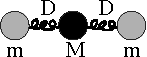
\includegraphics[width=0.20\textwidth]{CO2.pdf}
\end{center}
Die Koordinaten $\eta_i$ (mit $i = 1,2,3$) bezeichnen wie bisher die
Auslenkungen aus den Ruhelagen. Die kinetische Energie des Moleküls ist dann
\begin{equation}
T = \frac{m}{2}\left(\dot{\eta}_1^2 + \dot{\eta}_3^2\right) + \frac{M}{2}\dot{\eta}_2^2\,,
\end{equation}
die potentielle Energie in den Federn beträgt
\begin{equation}
V =\frac{1}{2}\left(\eta_2 - \eta_1\right)^2 + \frac{1}{2}D\left(\eta_3 - \eta_2\right)^2\,.
\end{equation}
Die $\mathbf T$- und $\mathbf V$-Matrizen lesen wir gemäß \eqref
{eq:Tapprox} und \eqref{eq:Vapprox} ab als
\begin{align}
T &= \begin{bmatrix}m & 0 & 0\\0 & M & 0\\ 0 & 0 & m\end{bmatrix}\,,\\
V &= D\threeMatrix{1}{-1}{0}{-1}{2}{-1}{0}{-1}{1}\,.
\end{align}
Die Frequenzen $\omega_r$ erhalten wir als Lösungen von Gleichung \eqref{eq:Det}.
Dieses Polynom lautet für unser CO\textsubscript{2}-Molekül
\begin{equation}
p(\omega^2) = \omega^{2} \left(- D + m \omega^{2}\right) \left(D M + 2 D m - M m \omega^{2}\right)\stackrel{!}{=}0\,,
\end{equation}
die drei zugehörigen Lösungen $\omega^2_r$ sowie die Amplituden $\vec A_r$ gemäß
\eqref{eq:EWlike} sind
\begin{enumerate}
    \item $\omega_1^2 = 0$. In diesem Fall ist
        \begin{equation}
            \vec A_1 = \DreierVec{1}{1}{1}\,.
        \end{equation}
        Die verschwindende Frequenz bedeutet, dass diese Lösung keine Vibration,
        sondern nur eine Translation ist.
    \item $\omega_2^2 = \frac{D}{m}$. Für diese Lösung ist
     \begin{equation}
            \vec A_2 = \DreierVec{1}{0}{-1}\,.
        \end{equation}
     Hier schwingen die beiden äußeren Atome gegenphasig mit gleicher
     Amplitude, während das zentrale Atom ruht.
    \item $\omega_3^2 = \frac{D}{m}+\frac{2D}{M}$. In diesem Fall ist
        \begin{equation}
            \vec A_3 = \DreierVec{1}{-2m/M}{1}\,.
        \end{equation}
        Hier schwingen also die beiden äußeren Atome in Phase (und mit
        gleicher Amplitude), dass mittlere Atome schwingt dazu gegenphasig
        mit (für $M < 2m$ wie in $\mathrm{CO}_2$) größerer Amplitude.
\end{enumerate}

\subsection{Normalkoordinaten}

Um die entsprechenden Normalkoordinaten zu finden, nutzen wir die Freiheit, die
Skalenfaktoren $C_r$ (bis hierher nicht mit aufgeführt) so zu wählen, dass
Gleichung \eqref{eq:Anorm} beziehungsweise für jeden Wert von $r$ die Gleichung
\begin{equation}
\vec A_r^\mathrm{T}\mathbf{T}\vec A_r = \frac{1}{C_r^2}
\end{equation}
erfüllt ist. Wir finden die Lösungen
\begin{align}
C_1 &= \frac{1}{\sqrt{M+2m}}\,,\\
C_2 &= \frac{1}{\sqrt{2m}}\,,\\
C_3 &= \frac{1}{\sqrt{2m\left(1+\frac{2m}{M}\right)}}\,.
\end{align}
Wenn wir damit die Vektoren $\vec A_r$ gemäß $\vec A_r \to \vec A_r' = C_r
\vec A_r$ neu normieren, so können wir nach \eqref{eq:AMatrix} die
Transformationsmatrix $\mathbf A = [\vec A_1', \dots, \vec A_s']$
aufschreiben und nach \eqref{eq:Normalkoordinaten} auf die Normalkoordinaten
$\vec Q$ transformieren. Mit $\mathbf{A}^{-1}=\mathbf{A}^{\mathrm{T}}\mathbf{T}$
ergeben sich
\begin{align}
Q_1 &= \frac{1}{\sqrt{M+2m}}(m\eta_1 + M\eta_2 + m\eta_3)\,,\\
Q_2 &= \sqrt{\frac{m}{2}}(\eta_1 - \eta_3)\,,\\
Q_3 &= \frac{mM}{\sqrt{2(M+2m)}}(\eta_1 - 2\eta_2 + \eta_3)\,.
\end{align}
In diesen Koordinaten schwingen entkoppeln die Bewegungsgleichungen, und im
Freiheitsgrad $Q_r$ ergibt sich eine harmonische Schwingung mit Frequenz
$\omega_r$. Die etwas mühselige Berechnung der Normalkoordinaten kann durch
Verwendung von \emph{Symmetrien} wesentlich vereinfacht werden, das könnte
Ihnen in der Molekülphysik wieder begegnen\dots

\subsection{Eine Bemerkung zum allgemeinen Fall}

Im Allgemeinen hat ein $N$-atomiges Molekül $3N$ Freiheitsgrade. Davon
entfallen $3$ auf Translationen des Schwerpunktes und $3$ auf Rotationen des
ganzen Moleküls. Es bleiben dann $3N - 3 - 3 = 3N-6$ Freiheitsgrade für
Schwingungen; es gibt also im Allgemeinen Fall auch $3N - 6$ Normalmoden,
oder -schwingungen.

Im unserem dreiatomigen CO\textsubscript{2}-Molekül wären das $3$
Normalschwingungen. Allerdings entfällt hier ein Freiheitsgrad für die
Rotationen -- Rotationen um die Molekülachse lassen die Konfiguration des
Moleküls unverändert; es gibt dann also $4$ Normalmoden. Zwei davon kennen
wir bereits, über die anderen beiden (Schwingungen \emph{senkrecht} zur
Molekülachse) können wir aufgrund der Symmetrie des Moleküls auf jeden Fall
sagen, dass sie entartet sein müssen! Das kommt daher, dass die beiden
unabhängigen (zueinander senkrechten) Richtungen senkrecht zur Längsachse
komplett gleichwertig sind.

Ein echtes Infrarot-Absorptionsspektrum von CO\textsubscript{2} ist in
Abbildung \ref{fig:Spektrum} gezeigt. Beachten Sie, dass die symmetrische
Schwingung mit Frequenz $\omega_2$ fehlt -- dies liegt daran, dass sich bei
dieser Schwingung das Dipolmoment des Moleküls nicht ändert.

\begin{figure}
    \centering
    %% Pgf figure exported from matplotlib.
%%
%% To include the image in your LaTeX document, write
%%   \input{<filename>.pgf}
%%
%% Make sure to load the required packages in your main document
%%   \usepackage{pgf}
%%
\begingroup%
\makeatletter%
\begin{pgfpicture}%
\pgfpathrectangle{\pgfpointorigin}{\pgfqpoint{5.000000in}{3.000000in}}%
\pgfusepath{use as bounding box}%
\begin{pgfscope}%
\pgfsetrectcap%
\pgfsetroundjoin%
\definecolor{currentfill}{rgb}{1.000000,1.000000,1.000000}%
\pgfsetfillcolor{currentfill}%
\pgfsetlinewidth{0.000000pt}%
\definecolor{currentstroke}{rgb}{1.000000,1.000000,1.000000}%
\pgfsetstrokecolor{currentstroke}%
\pgfsetdash{}{0pt}%
\pgfpathmoveto{\pgfqpoint{0.000000in}{0.000000in}}%
\pgfpathlineto{\pgfqpoint{5.000000in}{0.000000in}}%
\pgfpathlineto{\pgfqpoint{5.000000in}{3.000000in}}%
\pgfpathlineto{\pgfqpoint{0.000000in}{3.000000in}}%
\pgfpathclose%
\pgfusepath{fill}%
\end{pgfscope}%
\begin{pgfscope}%
\pgfsetrectcap%
\pgfsetroundjoin%
\definecolor{currentfill}{rgb}{1.000000,1.000000,1.000000}%
\pgfsetfillcolor{currentfill}%
\pgfsetlinewidth{0.000000pt}%
\definecolor{currentstroke}{rgb}{0.000000,0.000000,0.000000}%
\pgfsetstrokecolor{currentstroke}%
\pgfsetdash{}{0pt}%
\pgfpathmoveto{\pgfqpoint{0.625000in}{0.300000in}}%
\pgfpathlineto{\pgfqpoint{4.500000in}{0.300000in}}%
\pgfpathlineto{\pgfqpoint{4.500000in}{2.700000in}}%
\pgfpathlineto{\pgfqpoint{0.625000in}{2.700000in}}%
\pgfpathclose%
\pgfusepath{fill}%
\end{pgfscope}%
\begin{pgfscope}%
\pgfpathrectangle{\pgfqpoint{0.625000in}{0.300000in}}{\pgfqpoint{3.875000in}{2.400000in}} %
\pgfusepath{clip}%
\pgfsetrectcap%
\pgfsetroundjoin%
\pgfsetlinewidth{1.505625pt}%
\definecolor{currentstroke}{rgb}{0.000000,0.000000,1.000000}%
\pgfsetstrokecolor{currentstroke}%
\pgfsetdash{}{0pt}%
\pgfpathmoveto{\pgfqpoint{0.625000in}{2.484000in}}%
\pgfpathlineto{\pgfqpoint{0.641282in}{2.484000in}}%
\pgfpathlineto{\pgfqpoint{0.646709in}{2.486182in}}%
\pgfpathlineto{\pgfqpoint{0.668417in}{2.486182in}}%
\pgfpathlineto{\pgfqpoint{0.673845in}{2.484436in}}%
\pgfpathlineto{\pgfqpoint{0.679272in}{2.481818in}}%
\pgfpathlineto{\pgfqpoint{0.684699in}{2.475709in}}%
\pgfpathlineto{\pgfqpoint{0.690126in}{2.379709in}}%
\pgfpathlineto{\pgfqpoint{0.695553in}{2.146473in}}%
\pgfpathlineto{\pgfqpoint{0.700980in}{1.760727in}}%
\pgfpathlineto{\pgfqpoint{0.706408in}{1.542545in}}%
\pgfpathlineto{\pgfqpoint{0.711835in}{1.424509in}}%
\pgfpathlineto{\pgfqpoint{0.717262in}{1.366909in}}%
\pgfpathlineto{\pgfqpoint{0.722689in}{1.635709in}}%
\pgfpathlineto{\pgfqpoint{0.728116in}{1.989818in}}%
\pgfpathlineto{\pgfqpoint{0.733543in}{1.742182in}}%
\pgfpathlineto{\pgfqpoint{0.738971in}{1.590764in}}%
\pgfpathlineto{\pgfqpoint{0.744398in}{1.616291in}}%
\pgfpathlineto{\pgfqpoint{0.749825in}{1.701818in}}%
\pgfpathlineto{\pgfqpoint{0.755252in}{1.813309in}}%
\pgfpathlineto{\pgfqpoint{0.760679in}{2.015564in}}%
\pgfpathlineto{\pgfqpoint{0.766106in}{2.070764in}}%
\pgfpathlineto{\pgfqpoint{0.771534in}{2.226109in}}%
\pgfpathlineto{\pgfqpoint{0.787815in}{2.412218in}}%
\pgfpathlineto{\pgfqpoint{0.793242in}{2.431636in}}%
\pgfpathlineto{\pgfqpoint{0.798669in}{2.433818in}}%
\pgfpathlineto{\pgfqpoint{0.804097in}{2.386909in}}%
\pgfpathlineto{\pgfqpoint{0.809524in}{2.259709in}}%
\pgfpathlineto{\pgfqpoint{0.814951in}{1.949236in}}%
\pgfpathlineto{\pgfqpoint{0.820378in}{1.795636in}}%
\pgfpathlineto{\pgfqpoint{0.825805in}{1.671709in}}%
\pgfpathlineto{\pgfqpoint{0.831232in}{1.639200in}}%
\pgfpathlineto{\pgfqpoint{0.836660in}{1.824000in}}%
\pgfpathlineto{\pgfqpoint{0.842087in}{2.114836in}}%
\pgfpathlineto{\pgfqpoint{0.847514in}{2.136000in}}%
\pgfpathlineto{\pgfqpoint{0.852941in}{1.789745in}}%
\pgfpathlineto{\pgfqpoint{0.858368in}{1.749600in}}%
\pgfpathlineto{\pgfqpoint{0.863796in}{1.741745in}}%
\pgfpathlineto{\pgfqpoint{0.869223in}{1.828364in}}%
\pgfpathlineto{\pgfqpoint{0.874650in}{2.032364in}}%
\pgfpathlineto{\pgfqpoint{0.880077in}{2.167200in}}%
\pgfpathlineto{\pgfqpoint{0.885504in}{2.231782in}}%
\pgfpathlineto{\pgfqpoint{0.890931in}{2.255564in}}%
\pgfpathlineto{\pgfqpoint{0.896359in}{2.285455in}}%
\pgfpathlineto{\pgfqpoint{0.901786in}{2.336509in}}%
\pgfpathlineto{\pgfqpoint{0.912640in}{2.406545in}}%
\pgfpathlineto{\pgfqpoint{0.918067in}{2.430545in}}%
\pgfpathlineto{\pgfqpoint{0.923494in}{2.443418in}}%
\pgfpathlineto{\pgfqpoint{0.928922in}{2.451273in}}%
\pgfpathlineto{\pgfqpoint{0.934349in}{2.457818in}}%
\pgfpathlineto{\pgfqpoint{0.939776in}{2.462182in}}%
\pgfpathlineto{\pgfqpoint{0.945203in}{2.464582in}}%
\pgfpathlineto{\pgfqpoint{0.950630in}{2.469818in}}%
\pgfpathlineto{\pgfqpoint{0.956057in}{2.470909in}}%
\pgfpathlineto{\pgfqpoint{0.972339in}{2.477455in}}%
\pgfpathlineto{\pgfqpoint{0.977766in}{2.481600in}}%
\pgfpathlineto{\pgfqpoint{0.999475in}{2.481818in}}%
\pgfpathlineto{\pgfqpoint{1.032038in}{2.481818in}}%
\pgfpathlineto{\pgfqpoint{1.037465in}{2.484000in}}%
\pgfpathlineto{\pgfqpoint{1.211134in}{2.484000in}}%
\pgfpathlineto{\pgfqpoint{1.216562in}{2.481818in}}%
\pgfpathlineto{\pgfqpoint{1.254552in}{2.481818in}}%
\pgfpathlineto{\pgfqpoint{1.259979in}{2.477455in}}%
\pgfpathlineto{\pgfqpoint{1.373950in}{2.476800in}}%
\pgfpathlineto{\pgfqpoint{1.379377in}{2.475273in}}%
\pgfpathlineto{\pgfqpoint{1.384804in}{2.475273in}}%
\pgfpathlineto{\pgfqpoint{1.390231in}{2.471782in}}%
\pgfpathlineto{\pgfqpoint{1.395658in}{2.470909in}}%
\pgfpathlineto{\pgfqpoint{1.401085in}{2.470909in}}%
\pgfpathlineto{\pgfqpoint{1.406513in}{2.468727in}}%
\pgfpathlineto{\pgfqpoint{1.455357in}{2.468727in}}%
\pgfpathlineto{\pgfqpoint{1.460784in}{2.464364in}}%
\pgfpathlineto{\pgfqpoint{1.471639in}{2.464364in}}%
\pgfpathlineto{\pgfqpoint{1.482493in}{2.462182in}}%
\pgfpathlineto{\pgfqpoint{1.504202in}{2.462182in}}%
\pgfpathlineto{\pgfqpoint{1.509629in}{2.464364in}}%
\pgfpathlineto{\pgfqpoint{1.580182in}{2.464364in}}%
\pgfpathlineto{\pgfqpoint{1.585609in}{2.457818in}}%
\pgfpathlineto{\pgfqpoint{1.591036in}{2.457818in}}%
\pgfpathlineto{\pgfqpoint{1.596464in}{2.455636in}}%
\pgfpathlineto{\pgfqpoint{1.601891in}{2.455636in}}%
\pgfpathlineto{\pgfqpoint{1.607318in}{2.451273in}}%
\pgfpathlineto{\pgfqpoint{1.612745in}{2.449964in}}%
\pgfpathlineto{\pgfqpoint{1.618172in}{2.446909in}}%
\pgfpathlineto{\pgfqpoint{1.623599in}{2.448218in}}%
\pgfpathlineto{\pgfqpoint{1.629027in}{2.458473in}}%
\pgfpathlineto{\pgfqpoint{1.634454in}{2.479200in}}%
\pgfpathlineto{\pgfqpoint{1.639881in}{2.486400in}}%
\pgfpathlineto{\pgfqpoint{1.645308in}{2.490545in}}%
\pgfpathlineto{\pgfqpoint{1.650735in}{2.490327in}}%
\pgfpathlineto{\pgfqpoint{1.656162in}{2.485091in}}%
\pgfpathlineto{\pgfqpoint{1.661590in}{2.484000in}}%
\pgfpathlineto{\pgfqpoint{1.667017in}{2.481818in}}%
\pgfpathlineto{\pgfqpoint{1.672444in}{2.477455in}}%
\pgfpathlineto{\pgfqpoint{1.677871in}{2.477455in}}%
\pgfpathlineto{\pgfqpoint{1.683298in}{2.475273in}}%
\pgfpathlineto{\pgfqpoint{1.688725in}{2.470909in}}%
\pgfpathlineto{\pgfqpoint{1.694153in}{2.468727in}}%
\pgfpathlineto{\pgfqpoint{1.699580in}{2.463491in}}%
\pgfpathlineto{\pgfqpoint{1.705007in}{2.462182in}}%
\pgfpathlineto{\pgfqpoint{1.710434in}{2.463055in}}%
\pgfpathlineto{\pgfqpoint{1.715861in}{2.470036in}}%
\pgfpathlineto{\pgfqpoint{1.721289in}{2.484000in}}%
\pgfpathlineto{\pgfqpoint{1.726716in}{2.486182in}}%
\pgfpathlineto{\pgfqpoint{1.732143in}{2.486182in}}%
\pgfpathlineto{\pgfqpoint{1.737570in}{2.478764in}}%
\pgfpathlineto{\pgfqpoint{1.742997in}{2.477455in}}%
\pgfpathlineto{\pgfqpoint{1.911239in}{2.477455in}}%
\pgfpathlineto{\pgfqpoint{1.916667in}{2.475273in}}%
\pgfpathlineto{\pgfqpoint{1.927521in}{2.475273in}}%
\pgfpathlineto{\pgfqpoint{1.932948in}{2.477455in}}%
\pgfpathlineto{\pgfqpoint{1.943803in}{2.477455in}}%
\pgfpathlineto{\pgfqpoint{1.949230in}{2.481818in}}%
\pgfpathlineto{\pgfqpoint{1.954657in}{2.477455in}}%
\pgfpathlineto{\pgfqpoint{2.019783in}{2.477455in}}%
\pgfpathlineto{\pgfqpoint{2.030637in}{2.475273in}}%
\pgfpathlineto{\pgfqpoint{2.057773in}{2.475273in}}%
\pgfpathlineto{\pgfqpoint{2.063200in}{2.471564in}}%
\pgfpathlineto{\pgfqpoint{2.074055in}{2.470909in}}%
\pgfpathlineto{\pgfqpoint{2.095763in}{2.470909in}}%
\pgfpathlineto{\pgfqpoint{2.101190in}{2.468727in}}%
\pgfpathlineto{\pgfqpoint{2.193452in}{2.468727in}}%
\pgfpathlineto{\pgfqpoint{2.198880in}{2.464364in}}%
\pgfpathlineto{\pgfqpoint{2.215161in}{2.464364in}}%
\pgfpathlineto{\pgfqpoint{2.220588in}{2.468727in}}%
\pgfpathlineto{\pgfqpoint{2.226015in}{2.468727in}}%
\pgfpathlineto{\pgfqpoint{2.231443in}{2.464364in}}%
\pgfpathlineto{\pgfqpoint{2.236870in}{2.462182in}}%
\pgfpathlineto{\pgfqpoint{2.242297in}{2.456073in}}%
\pgfpathlineto{\pgfqpoint{2.247724in}{2.445600in}}%
\pgfpathlineto{\pgfqpoint{2.253151in}{2.067273in}}%
\pgfpathlineto{\pgfqpoint{2.258578in}{1.744364in}}%
\pgfpathlineto{\pgfqpoint{2.269433in}{0.385527in}}%
\pgfpathlineto{\pgfqpoint{2.274860in}{0.372000in}}%
\pgfpathlineto{\pgfqpoint{2.280287in}{0.367636in}}%
\pgfpathlineto{\pgfqpoint{2.291141in}{0.364582in}}%
\pgfpathlineto{\pgfqpoint{2.301996in}{0.350182in}}%
\pgfpathlineto{\pgfqpoint{2.307423in}{0.345818in}}%
\pgfpathlineto{\pgfqpoint{2.312850in}{0.345818in}}%
\pgfpathlineto{\pgfqpoint{2.323704in}{0.343636in}}%
\pgfpathlineto{\pgfqpoint{2.329132in}{0.339273in}}%
\pgfpathlineto{\pgfqpoint{2.334559in}{0.339709in}}%
\pgfpathlineto{\pgfqpoint{2.339986in}{0.344945in}}%
\pgfpathlineto{\pgfqpoint{2.345413in}{0.391855in}}%
\pgfpathlineto{\pgfqpoint{2.350840in}{0.536509in}}%
\pgfpathlineto{\pgfqpoint{2.356268in}{0.809673in}}%
\pgfpathlineto{\pgfqpoint{2.361695in}{0.859200in}}%
\pgfpathlineto{\pgfqpoint{2.367122in}{1.388509in}}%
\pgfpathlineto{\pgfqpoint{2.372549in}{1.559345in}}%
\pgfpathlineto{\pgfqpoint{2.377976in}{1.862836in}}%
\pgfpathlineto{\pgfqpoint{2.383403in}{1.742182in}}%
\pgfpathlineto{\pgfqpoint{2.388831in}{1.769455in}}%
\pgfpathlineto{\pgfqpoint{2.394258in}{1.806109in}}%
\pgfpathlineto{\pgfqpoint{2.399685in}{1.944873in}}%
\pgfpathlineto{\pgfqpoint{2.405112in}{1.889455in}}%
\pgfpathlineto{\pgfqpoint{2.410539in}{2.158036in}}%
\pgfpathlineto{\pgfqpoint{2.415966in}{2.106545in}}%
\pgfpathlineto{\pgfqpoint{2.421394in}{2.259709in}}%
\pgfpathlineto{\pgfqpoint{2.426821in}{2.361600in}}%
\pgfpathlineto{\pgfqpoint{2.432248in}{2.401964in}}%
\pgfpathlineto{\pgfqpoint{2.437675in}{2.429236in}}%
\pgfpathlineto{\pgfqpoint{2.448529in}{2.449745in}}%
\pgfpathlineto{\pgfqpoint{2.453957in}{2.454545in}}%
\pgfpathlineto{\pgfqpoint{2.464811in}{2.460873in}}%
\pgfpathlineto{\pgfqpoint{2.470238in}{2.462182in}}%
\pgfpathlineto{\pgfqpoint{2.475665in}{2.464364in}}%
\pgfpathlineto{\pgfqpoint{2.481092in}{2.468727in}}%
\pgfpathlineto{\pgfqpoint{2.502801in}{2.468291in}}%
\pgfpathlineto{\pgfqpoint{2.508228in}{2.464364in}}%
\pgfpathlineto{\pgfqpoint{2.513655in}{2.464364in}}%
\pgfpathlineto{\pgfqpoint{2.524510in}{2.462182in}}%
\pgfpathlineto{\pgfqpoint{2.546218in}{2.462182in}}%
\pgfpathlineto{\pgfqpoint{2.551646in}{2.457818in}}%
\pgfpathlineto{\pgfqpoint{2.567927in}{2.457818in}}%
\pgfpathlineto{\pgfqpoint{2.573354in}{2.460436in}}%
\pgfpathlineto{\pgfqpoint{2.578782in}{2.457818in}}%
\pgfpathlineto{\pgfqpoint{2.584209in}{2.462182in}}%
\pgfpathlineto{\pgfqpoint{2.589636in}{2.462182in}}%
\pgfpathlineto{\pgfqpoint{2.595063in}{2.460655in}}%
\pgfpathlineto{\pgfqpoint{2.600490in}{2.456073in}}%
\pgfpathlineto{\pgfqpoint{2.605917in}{2.455636in}}%
\pgfpathlineto{\pgfqpoint{2.611345in}{2.447782in}}%
\pgfpathlineto{\pgfqpoint{2.616772in}{2.444945in}}%
\pgfpathlineto{\pgfqpoint{2.622199in}{2.454545in}}%
\pgfpathlineto{\pgfqpoint{2.627626in}{2.457818in}}%
\pgfpathlineto{\pgfqpoint{2.633053in}{2.451273in}}%
\pgfpathlineto{\pgfqpoint{2.638480in}{2.450836in}}%
\pgfpathlineto{\pgfqpoint{2.643908in}{2.449091in}}%
\pgfpathlineto{\pgfqpoint{2.649335in}{2.451273in}}%
\pgfpathlineto{\pgfqpoint{2.660189in}{2.451927in}}%
\pgfpathlineto{\pgfqpoint{2.665616in}{2.455636in}}%
\pgfpathlineto{\pgfqpoint{2.671043in}{2.455855in}}%
\pgfpathlineto{\pgfqpoint{2.676471in}{2.457818in}}%
\pgfpathlineto{\pgfqpoint{2.747024in}{2.457818in}}%
\pgfpathlineto{\pgfqpoint{2.752451in}{2.455636in}}%
\pgfpathlineto{\pgfqpoint{2.757878in}{2.446909in}}%
\pgfpathlineto{\pgfqpoint{2.763305in}{2.442545in}}%
\pgfpathlineto{\pgfqpoint{2.768732in}{2.449091in}}%
\pgfpathlineto{\pgfqpoint{2.774160in}{2.446909in}}%
\pgfpathlineto{\pgfqpoint{2.785014in}{2.455636in}}%
\pgfpathlineto{\pgfqpoint{2.801296in}{2.455636in}}%
\pgfpathlineto{\pgfqpoint{2.806723in}{2.451273in}}%
\pgfpathlineto{\pgfqpoint{2.866422in}{2.451273in}}%
\pgfpathlineto{\pgfqpoint{2.871849in}{2.455636in}}%
\pgfpathlineto{\pgfqpoint{2.931548in}{2.455636in}}%
\pgfpathlineto{\pgfqpoint{2.936975in}{2.451273in}}%
\pgfpathlineto{\pgfqpoint{2.958683in}{2.451273in}}%
\pgfpathlineto{\pgfqpoint{2.964111in}{2.449091in}}%
\pgfpathlineto{\pgfqpoint{2.969538in}{2.451273in}}%
\pgfpathlineto{\pgfqpoint{2.980392in}{2.451273in}}%
\pgfpathlineto{\pgfqpoint{2.985819in}{2.449091in}}%
\pgfpathlineto{\pgfqpoint{3.002101in}{2.449091in}}%
\pgfpathlineto{\pgfqpoint{3.007528in}{2.446909in}}%
\pgfpathlineto{\pgfqpoint{3.012955in}{2.451273in}}%
\pgfpathlineto{\pgfqpoint{3.018382in}{2.451273in}}%
\pgfpathlineto{\pgfqpoint{3.023810in}{2.446909in}}%
\pgfpathlineto{\pgfqpoint{3.029237in}{2.446909in}}%
\pgfpathlineto{\pgfqpoint{3.040091in}{2.451273in}}%
\pgfpathlineto{\pgfqpoint{3.045518in}{2.455636in}}%
\pgfpathlineto{\pgfqpoint{3.050945in}{2.449091in}}%
\pgfpathlineto{\pgfqpoint{3.061800in}{2.449091in}}%
\pgfpathlineto{\pgfqpoint{3.067227in}{2.451273in}}%
\pgfpathlineto{\pgfqpoint{3.078081in}{2.464364in}}%
\pgfpathlineto{\pgfqpoint{3.083508in}{2.455636in}}%
\pgfpathlineto{\pgfqpoint{3.094363in}{2.455636in}}%
\pgfpathlineto{\pgfqpoint{3.099790in}{2.457818in}}%
\pgfpathlineto{\pgfqpoint{3.105217in}{2.457818in}}%
\pgfpathlineto{\pgfqpoint{3.121499in}{2.477455in}}%
\pgfpathlineto{\pgfqpoint{3.126926in}{2.475273in}}%
\pgfpathlineto{\pgfqpoint{3.137780in}{2.462182in}}%
\pgfpathlineto{\pgfqpoint{3.143207in}{2.462182in}}%
\pgfpathlineto{\pgfqpoint{3.148634in}{2.451273in}}%
\pgfpathlineto{\pgfqpoint{3.154062in}{2.457818in}}%
\pgfpathlineto{\pgfqpoint{3.159489in}{2.455636in}}%
\pgfpathlineto{\pgfqpoint{3.164916in}{2.457818in}}%
\pgfpathlineto{\pgfqpoint{3.170343in}{2.455636in}}%
\pgfpathlineto{\pgfqpoint{3.175770in}{2.457818in}}%
\pgfpathlineto{\pgfqpoint{3.186625in}{2.457818in}}%
\pgfpathlineto{\pgfqpoint{3.192052in}{2.455636in}}%
\pgfpathlineto{\pgfqpoint{3.197479in}{2.451273in}}%
\pgfpathlineto{\pgfqpoint{3.202906in}{2.455636in}}%
\pgfpathlineto{\pgfqpoint{3.208333in}{2.455636in}}%
\pgfpathlineto{\pgfqpoint{3.213761in}{2.457818in}}%
\pgfpathlineto{\pgfqpoint{3.219188in}{2.455636in}}%
\pgfpathlineto{\pgfqpoint{3.224615in}{2.455636in}}%
\pgfpathlineto{\pgfqpoint{3.230042in}{2.462182in}}%
\pgfpathlineto{\pgfqpoint{3.235469in}{2.455636in}}%
\pgfpathlineto{\pgfqpoint{3.240896in}{2.451273in}}%
\pgfpathlineto{\pgfqpoint{3.246324in}{2.455636in}}%
\pgfpathlineto{\pgfqpoint{3.251751in}{2.457818in}}%
\pgfpathlineto{\pgfqpoint{3.257178in}{2.455636in}}%
\pgfpathlineto{\pgfqpoint{3.262605in}{2.451273in}}%
\pgfpathlineto{\pgfqpoint{3.268032in}{2.451273in}}%
\pgfpathlineto{\pgfqpoint{3.273459in}{2.455636in}}%
\pgfpathlineto{\pgfqpoint{3.278887in}{2.462182in}}%
\pgfpathlineto{\pgfqpoint{3.284314in}{2.455636in}}%
\pgfpathlineto{\pgfqpoint{3.300595in}{2.455636in}}%
\pgfpathlineto{\pgfqpoint{3.306022in}{2.451273in}}%
\pgfpathlineto{\pgfqpoint{3.311450in}{2.451273in}}%
\pgfpathlineto{\pgfqpoint{3.316877in}{2.462182in}}%
\pgfpathlineto{\pgfqpoint{3.327731in}{2.462182in}}%
\pgfpathlineto{\pgfqpoint{3.333158in}{2.457818in}}%
\pgfpathlineto{\pgfqpoint{3.338585in}{2.451273in}}%
\pgfpathlineto{\pgfqpoint{3.349440in}{2.464364in}}%
\pgfpathlineto{\pgfqpoint{3.365721in}{2.464364in}}%
\pgfpathlineto{\pgfqpoint{3.371148in}{2.475273in}}%
\pgfpathlineto{\pgfqpoint{3.376576in}{2.470909in}}%
\pgfpathlineto{\pgfqpoint{3.382003in}{2.470909in}}%
\pgfpathlineto{\pgfqpoint{3.387430in}{2.477455in}}%
\pgfpathlineto{\pgfqpoint{3.392857in}{2.470909in}}%
\pgfpathlineto{\pgfqpoint{3.409139in}{2.470909in}}%
\pgfpathlineto{\pgfqpoint{3.414566in}{2.462182in}}%
\pgfpathlineto{\pgfqpoint{3.419993in}{2.422909in}}%
\pgfpathlineto{\pgfqpoint{3.425420in}{2.398909in}}%
\pgfpathlineto{\pgfqpoint{3.430847in}{2.422909in}}%
\pgfpathlineto{\pgfqpoint{3.436275in}{2.436000in}}%
\pgfpathlineto{\pgfqpoint{3.447129in}{2.449091in}}%
\pgfpathlineto{\pgfqpoint{3.452556in}{2.446909in}}%
\pgfpathlineto{\pgfqpoint{3.457983in}{2.451273in}}%
\pgfpathlineto{\pgfqpoint{3.463410in}{2.464364in}}%
\pgfpathlineto{\pgfqpoint{3.468838in}{2.475273in}}%
\pgfpathlineto{\pgfqpoint{3.474265in}{2.470909in}}%
\pgfpathlineto{\pgfqpoint{3.490546in}{2.470909in}}%
\pgfpathlineto{\pgfqpoint{3.495973in}{2.468727in}}%
\pgfpathlineto{\pgfqpoint{3.506828in}{2.468727in}}%
\pgfpathlineto{\pgfqpoint{3.512255in}{2.470909in}}%
\pgfpathlineto{\pgfqpoint{3.517682in}{2.470909in}}%
\pgfpathlineto{\pgfqpoint{3.523109in}{2.468727in}}%
\pgfpathlineto{\pgfqpoint{3.533964in}{2.468727in}}%
\pgfpathlineto{\pgfqpoint{3.539391in}{2.475273in}}%
\pgfpathlineto{\pgfqpoint{3.544818in}{2.475273in}}%
\pgfpathlineto{\pgfqpoint{3.550245in}{2.477455in}}%
\pgfpathlineto{\pgfqpoint{3.555672in}{2.477455in}}%
\pgfpathlineto{\pgfqpoint{3.561099in}{2.481818in}}%
\pgfpathlineto{\pgfqpoint{3.566527in}{2.481818in}}%
\pgfpathlineto{\pgfqpoint{3.571954in}{2.484000in}}%
\pgfpathlineto{\pgfqpoint{3.577381in}{2.484000in}}%
\pgfpathlineto{\pgfqpoint{3.582808in}{2.492727in}}%
\pgfpathlineto{\pgfqpoint{3.588235in}{2.499273in}}%
\pgfpathlineto{\pgfqpoint{3.599090in}{2.521091in}}%
\pgfpathlineto{\pgfqpoint{3.604517in}{2.525455in}}%
\pgfpathlineto{\pgfqpoint{3.609944in}{2.525455in}}%
\pgfpathlineto{\pgfqpoint{3.615371in}{2.527636in}}%
\pgfpathlineto{\pgfqpoint{3.620798in}{2.532000in}}%
\pgfpathlineto{\pgfqpoint{3.647934in}{2.532000in}}%
\pgfpathlineto{\pgfqpoint{3.658789in}{2.518909in}}%
\pgfpathlineto{\pgfqpoint{3.664216in}{2.505818in}}%
\pgfpathlineto{\pgfqpoint{3.669643in}{2.518909in}}%
\pgfpathlineto{\pgfqpoint{3.675070in}{2.521091in}}%
\pgfpathlineto{\pgfqpoint{3.691352in}{2.521091in}}%
\pgfpathlineto{\pgfqpoint{3.696779in}{2.518909in}}%
\pgfpathlineto{\pgfqpoint{3.707633in}{2.505818in}}%
\pgfpathlineto{\pgfqpoint{3.713060in}{2.510182in}}%
\pgfpathlineto{\pgfqpoint{3.718487in}{2.512364in}}%
\pgfpathlineto{\pgfqpoint{3.723915in}{2.518909in}}%
\pgfpathlineto{\pgfqpoint{3.729342in}{2.521091in}}%
\pgfpathlineto{\pgfqpoint{3.740196in}{2.521091in}}%
\pgfpathlineto{\pgfqpoint{3.745623in}{2.518909in}}%
\pgfpathlineto{\pgfqpoint{3.756478in}{2.518909in}}%
\pgfpathlineto{\pgfqpoint{3.761905in}{2.514545in}}%
\pgfpathlineto{\pgfqpoint{3.772759in}{2.510182in}}%
\pgfpathlineto{\pgfqpoint{3.778186in}{2.503636in}}%
\pgfpathlineto{\pgfqpoint{3.783613in}{2.490545in}}%
\pgfpathlineto{\pgfqpoint{3.789041in}{2.492727in}}%
\pgfpathlineto{\pgfqpoint{3.794468in}{2.505818in}}%
\pgfpathlineto{\pgfqpoint{3.799895in}{2.510182in}}%
\pgfpathlineto{\pgfqpoint{3.805322in}{2.510182in}}%
\pgfpathlineto{\pgfqpoint{3.810749in}{2.490545in}}%
\pgfpathlineto{\pgfqpoint{3.816176in}{2.514545in}}%
\pgfpathlineto{\pgfqpoint{3.821604in}{2.505818in}}%
\pgfpathlineto{\pgfqpoint{3.827031in}{2.514545in}}%
\pgfpathlineto{\pgfqpoint{3.832458in}{2.514545in}}%
\pgfpathlineto{\pgfqpoint{3.837885in}{2.512364in}}%
\pgfpathlineto{\pgfqpoint{3.843312in}{2.512364in}}%
\pgfpathlineto{\pgfqpoint{3.848739in}{2.510182in}}%
\pgfpathlineto{\pgfqpoint{3.854167in}{2.503636in}}%
\pgfpathlineto{\pgfqpoint{3.859594in}{2.499273in}}%
\pgfpathlineto{\pgfqpoint{3.865021in}{2.490545in}}%
\pgfpathlineto{\pgfqpoint{3.870448in}{2.499273in}}%
\pgfpathlineto{\pgfqpoint{3.875875in}{2.503636in}}%
\pgfpathlineto{\pgfqpoint{3.881303in}{2.499273in}}%
\pgfpathlineto{\pgfqpoint{3.886730in}{2.497091in}}%
\pgfpathlineto{\pgfqpoint{3.892157in}{2.497091in}}%
\pgfpathlineto{\pgfqpoint{3.897584in}{2.499273in}}%
\pgfpathlineto{\pgfqpoint{3.903011in}{2.497091in}}%
\pgfpathlineto{\pgfqpoint{3.908438in}{2.497091in}}%
\pgfpathlineto{\pgfqpoint{3.913866in}{2.492727in}}%
\pgfpathlineto{\pgfqpoint{3.941001in}{2.492727in}}%
\pgfpathlineto{\pgfqpoint{3.946429in}{2.490545in}}%
\pgfpathlineto{\pgfqpoint{3.951856in}{2.490545in}}%
\pgfpathlineto{\pgfqpoint{3.957283in}{2.486182in}}%
\pgfpathlineto{\pgfqpoint{3.962710in}{2.486182in}}%
\pgfpathlineto{\pgfqpoint{3.973564in}{2.481818in}}%
\pgfpathlineto{\pgfqpoint{3.978992in}{2.475273in}}%
\pgfpathlineto{\pgfqpoint{3.984419in}{2.470909in}}%
\pgfpathlineto{\pgfqpoint{3.989846in}{2.475273in}}%
\pgfpathlineto{\pgfqpoint{3.995273in}{2.470909in}}%
\pgfpathlineto{\pgfqpoint{4.000700in}{2.470909in}}%
\pgfpathlineto{\pgfqpoint{4.006127in}{2.475273in}}%
\pgfpathlineto{\pgfqpoint{4.011555in}{2.470909in}}%
\pgfpathlineto{\pgfqpoint{4.022409in}{2.470909in}}%
\pgfpathlineto{\pgfqpoint{4.027836in}{2.468727in}}%
\pgfpathlineto{\pgfqpoint{4.038690in}{2.468727in}}%
\pgfpathlineto{\pgfqpoint{4.044118in}{2.470909in}}%
\pgfpathlineto{\pgfqpoint{4.049545in}{2.468727in}}%
\pgfpathlineto{\pgfqpoint{4.054972in}{2.468727in}}%
\pgfpathlineto{\pgfqpoint{4.060399in}{2.464364in}}%
\pgfpathlineto{\pgfqpoint{4.065826in}{2.462182in}}%
\pgfpathlineto{\pgfqpoint{4.071254in}{2.464364in}}%
\pgfpathlineto{\pgfqpoint{4.076681in}{2.462182in}}%
\pgfpathlineto{\pgfqpoint{4.082108in}{2.462182in}}%
\pgfpathlineto{\pgfqpoint{4.087535in}{2.457818in}}%
\pgfpathlineto{\pgfqpoint{4.092962in}{2.457818in}}%
\pgfpathlineto{\pgfqpoint{4.098389in}{2.455636in}}%
\pgfpathlineto{\pgfqpoint{4.103817in}{2.455636in}}%
\pgfpathlineto{\pgfqpoint{4.109244in}{2.457818in}}%
\pgfpathlineto{\pgfqpoint{4.120098in}{2.457818in}}%
\pgfpathlineto{\pgfqpoint{4.125525in}{2.464364in}}%
\pgfpathlineto{\pgfqpoint{4.130952in}{2.462182in}}%
\pgfpathlineto{\pgfqpoint{4.136380in}{2.462182in}}%
\pgfpathlineto{\pgfqpoint{4.141807in}{2.457818in}}%
\pgfpathlineto{\pgfqpoint{4.147234in}{2.451273in}}%
\pgfpathlineto{\pgfqpoint{4.152661in}{2.442545in}}%
\pgfpathlineto{\pgfqpoint{4.158088in}{2.429455in}}%
\pgfpathlineto{\pgfqpoint{4.163515in}{2.401091in}}%
\pgfpathlineto{\pgfqpoint{4.168943in}{2.313818in}}%
\pgfpathlineto{\pgfqpoint{4.179797in}{2.326909in}}%
\pgfpathlineto{\pgfqpoint{4.185224in}{2.348727in}}%
\pgfpathlineto{\pgfqpoint{4.190651in}{2.389745in}}%
\pgfpathlineto{\pgfqpoint{4.196078in}{2.077964in}}%
\pgfpathlineto{\pgfqpoint{4.201506in}{2.213455in}}%
\pgfpathlineto{\pgfqpoint{4.206933in}{2.065091in}}%
\pgfpathlineto{\pgfqpoint{4.217787in}{1.633091in}}%
\pgfpathlineto{\pgfqpoint{4.223214in}{1.380000in}}%
\pgfpathlineto{\pgfqpoint{4.228641in}{1.196727in}}%
\pgfpathlineto{\pgfqpoint{4.234069in}{1.048364in}}%
\pgfpathlineto{\pgfqpoint{4.239496in}{0.967636in}}%
\pgfpathlineto{\pgfqpoint{4.244923in}{0.910909in}}%
\pgfpathlineto{\pgfqpoint{4.250350in}{0.952364in}}%
\pgfpathlineto{\pgfqpoint{4.255777in}{0.592582in}}%
\pgfpathlineto{\pgfqpoint{4.261204in}{1.140000in}}%
\pgfpathlineto{\pgfqpoint{4.266632in}{1.076727in}}%
\pgfpathlineto{\pgfqpoint{4.272059in}{1.052727in}}%
\pgfpathlineto{\pgfqpoint{4.277486in}{0.961309in}}%
\pgfpathlineto{\pgfqpoint{4.282913in}{1.408364in}}%
\pgfpathlineto{\pgfqpoint{4.288340in}{1.585309in}}%
\pgfpathlineto{\pgfqpoint{4.299195in}{2.058764in}}%
\pgfpathlineto{\pgfqpoint{4.304622in}{2.270182in}}%
\pgfpathlineto{\pgfqpoint{4.310049in}{2.360291in}}%
\pgfpathlineto{\pgfqpoint{4.315476in}{2.357455in}}%
\pgfpathlineto{\pgfqpoint{4.320903in}{2.342182in}}%
\pgfpathlineto{\pgfqpoint{4.326331in}{2.335636in}}%
\pgfpathlineto{\pgfqpoint{4.331758in}{2.350909in}}%
\pgfpathlineto{\pgfqpoint{4.337185in}{2.326909in}}%
\pgfpathlineto{\pgfqpoint{4.342612in}{2.394545in}}%
\pgfpathlineto{\pgfqpoint{4.348039in}{2.414182in}}%
\pgfpathlineto{\pgfqpoint{4.353466in}{2.422909in}}%
\pgfpathlineto{\pgfqpoint{4.358894in}{2.429455in}}%
\pgfpathlineto{\pgfqpoint{4.364321in}{2.433818in}}%
\pgfpathlineto{\pgfqpoint{4.369748in}{2.427273in}}%
\pgfpathlineto{\pgfqpoint{4.380602in}{2.418545in}}%
\pgfpathlineto{\pgfqpoint{4.386029in}{2.407636in}}%
\pgfpathlineto{\pgfqpoint{4.391457in}{2.398909in}}%
\pgfpathlineto{\pgfqpoint{4.396884in}{2.398909in}}%
\pgfpathlineto{\pgfqpoint{4.402311in}{2.405455in}}%
\pgfpathlineto{\pgfqpoint{4.418592in}{2.405455in}}%
\pgfpathlineto{\pgfqpoint{4.424020in}{2.407636in}}%
\pgfpathlineto{\pgfqpoint{4.429447in}{2.405455in}}%
\pgfpathlineto{\pgfqpoint{4.434874in}{2.398909in}}%
\pgfpathlineto{\pgfqpoint{4.440301in}{2.405455in}}%
\pgfpathlineto{\pgfqpoint{4.445728in}{2.414182in}}%
\pgfpathlineto{\pgfqpoint{4.462010in}{2.427273in}}%
\pgfpathlineto{\pgfqpoint{4.467437in}{2.427273in}}%
\pgfpathlineto{\pgfqpoint{4.472864in}{2.429455in}}%
\pgfpathlineto{\pgfqpoint{4.478291in}{2.436000in}}%
\pgfpathlineto{\pgfqpoint{4.483718in}{2.433818in}}%
\pgfpathlineto{\pgfqpoint{4.494573in}{2.420727in}}%
\pgfpathlineto{\pgfqpoint{4.500000in}{2.422909in}}%
\pgfpathlineto{\pgfqpoint{4.500000in}{2.422909in}}%
\pgfusepath{stroke}%
\end{pgfscope}%
\begin{pgfscope}%
\pgfsetbuttcap%
\pgfsetroundjoin%
\definecolor{currentfill}{rgb}{0.000000,0.000000,0.000000}%
\pgfsetfillcolor{currentfill}%
\pgfsetlinewidth{0.501875pt}%
\definecolor{currentstroke}{rgb}{0.000000,0.000000,0.000000}%
\pgfsetstrokecolor{currentstroke}%
\pgfsetdash{}{0pt}%
\pgfsys@defobject{currentmarker}{\pgfqpoint{0.000000in}{0.000000in}}{\pgfqpoint{0.000000in}{0.026667in}}{%
\pgfpathmoveto{\pgfqpoint{0.000000in}{0.000000in}}%
\pgfpathlineto{\pgfqpoint{0.000000in}{0.026667in}}%
\pgfusepath{stroke,fill}%
}%
\begin{pgfscope}%
\pgfsys@transformshift{4.452242in}{0.300000in}%
\pgfsys@useobject{currentmarker}{}%
\end{pgfscope}%
\end{pgfscope}%
\begin{pgfscope}%
\pgfsetbuttcap%
\pgfsetroundjoin%
\definecolor{currentfill}{rgb}{0.000000,0.000000,0.000000}%
\pgfsetfillcolor{currentfill}%
\pgfsetlinewidth{0.501875pt}%
\definecolor{currentstroke}{rgb}{0.000000,0.000000,0.000000}%
\pgfsetstrokecolor{currentstroke}%
\pgfsetdash{}{0pt}%
\pgfsys@defobject{currentmarker}{\pgfqpoint{0.000000in}{-0.026667in}}{\pgfqpoint{0.000000in}{0.000000in}}{%
\pgfpathmoveto{\pgfqpoint{0.000000in}{0.000000in}}%
\pgfpathlineto{\pgfqpoint{0.000000in}{-0.026667in}}%
\pgfusepath{stroke,fill}%
}%
\begin{pgfscope}%
\pgfsys@transformshift{4.452242in}{2.700000in}%
\pgfsys@useobject{currentmarker}{}%
\end{pgfscope}%
\end{pgfscope}%
\begin{pgfscope}%
\pgftext[left,bottom,x=4.329847in,y=0.137037in,rotate=0.000000]{{\rmfamily\fontsize{12.000000}{14.400000}\selectfont \(\displaystyle 500\)}}
%
\end{pgfscope}%
\begin{pgfscope}%
\pgfsetbuttcap%
\pgfsetroundjoin%
\definecolor{currentfill}{rgb}{0.000000,0.000000,0.000000}%
\pgfsetfillcolor{currentfill}%
\pgfsetlinewidth{0.501875pt}%
\definecolor{currentstroke}{rgb}{0.000000,0.000000,0.000000}%
\pgfsetstrokecolor{currentstroke}%
\pgfsetdash{}{0pt}%
\pgfsys@defobject{currentmarker}{\pgfqpoint{0.000000in}{0.000000in}}{\pgfqpoint{0.000000in}{0.026667in}}{%
\pgfpathmoveto{\pgfqpoint{0.000000in}{0.000000in}}%
\pgfpathlineto{\pgfqpoint{0.000000in}{0.026667in}}%
\pgfusepath{stroke,fill}%
}%
\begin{pgfscope}%
\pgfsys@transformshift{3.871536in}{0.300000in}%
\pgfsys@useobject{currentmarker}{}%
\end{pgfscope}%
\end{pgfscope}%
\begin{pgfscope}%
\pgfsetbuttcap%
\pgfsetroundjoin%
\definecolor{currentfill}{rgb}{0.000000,0.000000,0.000000}%
\pgfsetfillcolor{currentfill}%
\pgfsetlinewidth{0.501875pt}%
\definecolor{currentstroke}{rgb}{0.000000,0.000000,0.000000}%
\pgfsetstrokecolor{currentstroke}%
\pgfsetdash{}{0pt}%
\pgfsys@defobject{currentmarker}{\pgfqpoint{0.000000in}{-0.026667in}}{\pgfqpoint{0.000000in}{0.000000in}}{%
\pgfpathmoveto{\pgfqpoint{0.000000in}{0.000000in}}%
\pgfpathlineto{\pgfqpoint{0.000000in}{-0.026667in}}%
\pgfusepath{stroke,fill}%
}%
\begin{pgfscope}%
\pgfsys@transformshift{3.871536in}{2.700000in}%
\pgfsys@useobject{currentmarker}{}%
\end{pgfscope}%
\end{pgfscope}%
\begin{pgfscope}%
\pgftext[left,bottom,x=3.708343in,y=0.137037in,rotate=0.000000]{{\rmfamily\fontsize{12.000000}{14.400000}\selectfont \(\displaystyle 1000\)}}
%
\end{pgfscope}%
\begin{pgfscope}%
\pgfsetbuttcap%
\pgfsetroundjoin%
\definecolor{currentfill}{rgb}{0.000000,0.000000,0.000000}%
\pgfsetfillcolor{currentfill}%
\pgfsetlinewidth{0.501875pt}%
\definecolor{currentstroke}{rgb}{0.000000,0.000000,0.000000}%
\pgfsetstrokecolor{currentstroke}%
\pgfsetdash{}{0pt}%
\pgfsys@defobject{currentmarker}{\pgfqpoint{0.000000in}{0.000000in}}{\pgfqpoint{0.000000in}{0.026667in}}{%
\pgfpathmoveto{\pgfqpoint{0.000000in}{0.000000in}}%
\pgfpathlineto{\pgfqpoint{0.000000in}{0.026667in}}%
\pgfusepath{stroke,fill}%
}%
\begin{pgfscope}%
\pgfsys@transformshift{3.290831in}{0.300000in}%
\pgfsys@useobject{currentmarker}{}%
\end{pgfscope}%
\end{pgfscope}%
\begin{pgfscope}%
\pgfsetbuttcap%
\pgfsetroundjoin%
\definecolor{currentfill}{rgb}{0.000000,0.000000,0.000000}%
\pgfsetfillcolor{currentfill}%
\pgfsetlinewidth{0.501875pt}%
\definecolor{currentstroke}{rgb}{0.000000,0.000000,0.000000}%
\pgfsetstrokecolor{currentstroke}%
\pgfsetdash{}{0pt}%
\pgfsys@defobject{currentmarker}{\pgfqpoint{0.000000in}{-0.026667in}}{\pgfqpoint{0.000000in}{0.000000in}}{%
\pgfpathmoveto{\pgfqpoint{0.000000in}{0.000000in}}%
\pgfpathlineto{\pgfqpoint{0.000000in}{-0.026667in}}%
\pgfusepath{stroke,fill}%
}%
\begin{pgfscope}%
\pgfsys@transformshift{3.290831in}{2.700000in}%
\pgfsys@useobject{currentmarker}{}%
\end{pgfscope}%
\end{pgfscope}%
\begin{pgfscope}%
\pgftext[left,bottom,x=3.127638in,y=0.137037in,rotate=0.000000]{{\rmfamily\fontsize{12.000000}{14.400000}\selectfont \(\displaystyle 1500\)}}
%
\end{pgfscope}%
\begin{pgfscope}%
\pgfsetbuttcap%
\pgfsetroundjoin%
\definecolor{currentfill}{rgb}{0.000000,0.000000,0.000000}%
\pgfsetfillcolor{currentfill}%
\pgfsetlinewidth{0.501875pt}%
\definecolor{currentstroke}{rgb}{0.000000,0.000000,0.000000}%
\pgfsetstrokecolor{currentstroke}%
\pgfsetdash{}{0pt}%
\pgfsys@defobject{currentmarker}{\pgfqpoint{0.000000in}{0.000000in}}{\pgfqpoint{0.000000in}{0.026667in}}{%
\pgfpathmoveto{\pgfqpoint{0.000000in}{0.000000in}}%
\pgfpathlineto{\pgfqpoint{0.000000in}{0.026667in}}%
\pgfusepath{stroke,fill}%
}%
\begin{pgfscope}%
\pgfsys@transformshift{2.710125in}{0.300000in}%
\pgfsys@useobject{currentmarker}{}%
\end{pgfscope}%
\end{pgfscope}%
\begin{pgfscope}%
\pgfsetbuttcap%
\pgfsetroundjoin%
\definecolor{currentfill}{rgb}{0.000000,0.000000,0.000000}%
\pgfsetfillcolor{currentfill}%
\pgfsetlinewidth{0.501875pt}%
\definecolor{currentstroke}{rgb}{0.000000,0.000000,0.000000}%
\pgfsetstrokecolor{currentstroke}%
\pgfsetdash{}{0pt}%
\pgfsys@defobject{currentmarker}{\pgfqpoint{0.000000in}{-0.026667in}}{\pgfqpoint{0.000000in}{0.000000in}}{%
\pgfpathmoveto{\pgfqpoint{0.000000in}{0.000000in}}%
\pgfpathlineto{\pgfqpoint{0.000000in}{-0.026667in}}%
\pgfusepath{stroke,fill}%
}%
\begin{pgfscope}%
\pgfsys@transformshift{2.710125in}{2.700000in}%
\pgfsys@useobject{currentmarker}{}%
\end{pgfscope}%
\end{pgfscope}%
\begin{pgfscope}%
\pgftext[left,bottom,x=2.546932in,y=0.137037in,rotate=0.000000]{{\rmfamily\fontsize{12.000000}{14.400000}\selectfont \(\displaystyle 2000\)}}
%
\end{pgfscope}%
\begin{pgfscope}%
\pgfsetbuttcap%
\pgfsetroundjoin%
\definecolor{currentfill}{rgb}{0.000000,0.000000,0.000000}%
\pgfsetfillcolor{currentfill}%
\pgfsetlinewidth{0.501875pt}%
\definecolor{currentstroke}{rgb}{0.000000,0.000000,0.000000}%
\pgfsetstrokecolor{currentstroke}%
\pgfsetdash{}{0pt}%
\pgfsys@defobject{currentmarker}{\pgfqpoint{0.000000in}{0.000000in}}{\pgfqpoint{0.000000in}{0.026667in}}{%
\pgfpathmoveto{\pgfqpoint{0.000000in}{0.000000in}}%
\pgfpathlineto{\pgfqpoint{0.000000in}{0.026667in}}%
\pgfusepath{stroke,fill}%
}%
\begin{pgfscope}%
\pgfsys@transformshift{2.129420in}{0.300000in}%
\pgfsys@useobject{currentmarker}{}%
\end{pgfscope}%
\end{pgfscope}%
\begin{pgfscope}%
\pgfsetbuttcap%
\pgfsetroundjoin%
\definecolor{currentfill}{rgb}{0.000000,0.000000,0.000000}%
\pgfsetfillcolor{currentfill}%
\pgfsetlinewidth{0.501875pt}%
\definecolor{currentstroke}{rgb}{0.000000,0.000000,0.000000}%
\pgfsetstrokecolor{currentstroke}%
\pgfsetdash{}{0pt}%
\pgfsys@defobject{currentmarker}{\pgfqpoint{0.000000in}{-0.026667in}}{\pgfqpoint{0.000000in}{0.000000in}}{%
\pgfpathmoveto{\pgfqpoint{0.000000in}{0.000000in}}%
\pgfpathlineto{\pgfqpoint{0.000000in}{-0.026667in}}%
\pgfusepath{stroke,fill}%
}%
\begin{pgfscope}%
\pgfsys@transformshift{2.129420in}{2.700000in}%
\pgfsys@useobject{currentmarker}{}%
\end{pgfscope}%
\end{pgfscope}%
\begin{pgfscope}%
\pgftext[left,bottom,x=1.966227in,y=0.137037in,rotate=0.000000]{{\rmfamily\fontsize{12.000000}{14.400000}\selectfont \(\displaystyle 2500\)}}
%
\end{pgfscope}%
\begin{pgfscope}%
\pgfsetbuttcap%
\pgfsetroundjoin%
\definecolor{currentfill}{rgb}{0.000000,0.000000,0.000000}%
\pgfsetfillcolor{currentfill}%
\pgfsetlinewidth{0.501875pt}%
\definecolor{currentstroke}{rgb}{0.000000,0.000000,0.000000}%
\pgfsetstrokecolor{currentstroke}%
\pgfsetdash{}{0pt}%
\pgfsys@defobject{currentmarker}{\pgfqpoint{0.000000in}{0.000000in}}{\pgfqpoint{0.000000in}{0.026667in}}{%
\pgfpathmoveto{\pgfqpoint{0.000000in}{0.000000in}}%
\pgfpathlineto{\pgfqpoint{0.000000in}{0.026667in}}%
\pgfusepath{stroke,fill}%
}%
\begin{pgfscope}%
\pgfsys@transformshift{1.548714in}{0.300000in}%
\pgfsys@useobject{currentmarker}{}%
\end{pgfscope}%
\end{pgfscope}%
\begin{pgfscope}%
\pgfsetbuttcap%
\pgfsetroundjoin%
\definecolor{currentfill}{rgb}{0.000000,0.000000,0.000000}%
\pgfsetfillcolor{currentfill}%
\pgfsetlinewidth{0.501875pt}%
\definecolor{currentstroke}{rgb}{0.000000,0.000000,0.000000}%
\pgfsetstrokecolor{currentstroke}%
\pgfsetdash{}{0pt}%
\pgfsys@defobject{currentmarker}{\pgfqpoint{0.000000in}{-0.026667in}}{\pgfqpoint{0.000000in}{0.000000in}}{%
\pgfpathmoveto{\pgfqpoint{0.000000in}{0.000000in}}%
\pgfpathlineto{\pgfqpoint{0.000000in}{-0.026667in}}%
\pgfusepath{stroke,fill}%
}%
\begin{pgfscope}%
\pgfsys@transformshift{1.548714in}{2.700000in}%
\pgfsys@useobject{currentmarker}{}%
\end{pgfscope}%
\end{pgfscope}%
\begin{pgfscope}%
\pgftext[left,bottom,x=1.385522in,y=0.137037in,rotate=0.000000]{{\rmfamily\fontsize{12.000000}{14.400000}\selectfont \(\displaystyle 3000\)}}
%
\end{pgfscope}%
\begin{pgfscope}%
\pgfsetbuttcap%
\pgfsetroundjoin%
\definecolor{currentfill}{rgb}{0.000000,0.000000,0.000000}%
\pgfsetfillcolor{currentfill}%
\pgfsetlinewidth{0.501875pt}%
\definecolor{currentstroke}{rgb}{0.000000,0.000000,0.000000}%
\pgfsetstrokecolor{currentstroke}%
\pgfsetdash{}{0pt}%
\pgfsys@defobject{currentmarker}{\pgfqpoint{0.000000in}{0.000000in}}{\pgfqpoint{0.000000in}{0.026667in}}{%
\pgfpathmoveto{\pgfqpoint{0.000000in}{0.000000in}}%
\pgfpathlineto{\pgfqpoint{0.000000in}{0.026667in}}%
\pgfusepath{stroke,fill}%
}%
\begin{pgfscope}%
\pgfsys@transformshift{0.968009in}{0.300000in}%
\pgfsys@useobject{currentmarker}{}%
\end{pgfscope}%
\end{pgfscope}%
\begin{pgfscope}%
\pgfsetbuttcap%
\pgfsetroundjoin%
\definecolor{currentfill}{rgb}{0.000000,0.000000,0.000000}%
\pgfsetfillcolor{currentfill}%
\pgfsetlinewidth{0.501875pt}%
\definecolor{currentstroke}{rgb}{0.000000,0.000000,0.000000}%
\pgfsetstrokecolor{currentstroke}%
\pgfsetdash{}{0pt}%
\pgfsys@defobject{currentmarker}{\pgfqpoint{0.000000in}{-0.026667in}}{\pgfqpoint{0.000000in}{0.000000in}}{%
\pgfpathmoveto{\pgfqpoint{0.000000in}{0.000000in}}%
\pgfpathlineto{\pgfqpoint{0.000000in}{-0.026667in}}%
\pgfusepath{stroke,fill}%
}%
\begin{pgfscope}%
\pgfsys@transformshift{0.968009in}{2.700000in}%
\pgfsys@useobject{currentmarker}{}%
\end{pgfscope}%
\end{pgfscope}%
\begin{pgfscope}%
\pgftext[left,bottom,x=0.804816in,y=0.137037in,rotate=0.000000]{{\rmfamily\fontsize{12.000000}{14.400000}\selectfont \(\displaystyle 3500\)}}
%
\end{pgfscope}%
\begin{pgfscope}%
\pgftext[left,bottom,x=2.274897in,y=-0.114494in,rotate=0.000000]{{\rmfamily\fontsize{12.000000}{14.400000}\selectfont \(\displaystyle k\,[\mathrm{cm}^{-1}]\)}}
%
\end{pgfscope}%
\begin{pgfscope}%
\pgfsetbuttcap%
\pgfsetroundjoin%
\definecolor{currentfill}{rgb}{0.000000,0.000000,0.000000}%
\pgfsetfillcolor{currentfill}%
\pgfsetlinewidth{0.501875pt}%
\definecolor{currentstroke}{rgb}{0.000000,0.000000,0.000000}%
\pgfsetstrokecolor{currentstroke}%
\pgfsetdash{}{0pt}%
\pgfsys@defobject{currentmarker}{\pgfqpoint{0.000000in}{0.000000in}}{\pgfqpoint{0.026667in}{0.000000in}}{%
\pgfpathmoveto{\pgfqpoint{0.000000in}{0.000000in}}%
\pgfpathlineto{\pgfqpoint{0.026667in}{0.000000in}}%
\pgfusepath{stroke,fill}%
}%
\begin{pgfscope}%
\pgfsys@transformshift{0.625000in}{0.300000in}%
\pgfsys@useobject{currentmarker}{}%
\end{pgfscope}%
\end{pgfscope}%
\begin{pgfscope}%
\pgfsetbuttcap%
\pgfsetroundjoin%
\definecolor{currentfill}{rgb}{0.000000,0.000000,0.000000}%
\pgfsetfillcolor{currentfill}%
\pgfsetlinewidth{0.501875pt}%
\definecolor{currentstroke}{rgb}{0.000000,0.000000,0.000000}%
\pgfsetstrokecolor{currentstroke}%
\pgfsetdash{}{0pt}%
\pgfsys@defobject{currentmarker}{\pgfqpoint{-0.026667in}{0.000000in}}{\pgfqpoint{0.000000in}{0.000000in}}{%
\pgfpathmoveto{\pgfqpoint{0.000000in}{0.000000in}}%
\pgfpathlineto{\pgfqpoint{-0.026667in}{0.000000in}}%
\pgfusepath{stroke,fill}%
}%
\begin{pgfscope}%
\pgfsys@transformshift{4.500000in}{0.300000in}%
\pgfsys@useobject{currentmarker}{}%
\end{pgfscope}%
\end{pgfscope}%
\begin{pgfscope}%
\pgftext[left,bottom,x=0.360920in,y=0.246296in,rotate=0.000000]{{\rmfamily\fontsize{12.000000}{14.400000}\selectfont \(\displaystyle 0.0\)}}
%
\end{pgfscope}%
\begin{pgfscope}%
\pgfsetbuttcap%
\pgfsetroundjoin%
\definecolor{currentfill}{rgb}{0.000000,0.000000,0.000000}%
\pgfsetfillcolor{currentfill}%
\pgfsetlinewidth{0.501875pt}%
\definecolor{currentstroke}{rgb}{0.000000,0.000000,0.000000}%
\pgfsetstrokecolor{currentstroke}%
\pgfsetdash{}{0pt}%
\pgfsys@defobject{currentmarker}{\pgfqpoint{0.000000in}{0.000000in}}{\pgfqpoint{0.026667in}{0.000000in}}{%
\pgfpathmoveto{\pgfqpoint{0.000000in}{0.000000in}}%
\pgfpathlineto{\pgfqpoint{0.026667in}{0.000000in}}%
\pgfusepath{stroke,fill}%
}%
\begin{pgfscope}%
\pgfsys@transformshift{0.625000in}{0.736364in}%
\pgfsys@useobject{currentmarker}{}%
\end{pgfscope}%
\end{pgfscope}%
\begin{pgfscope}%
\pgfsetbuttcap%
\pgfsetroundjoin%
\definecolor{currentfill}{rgb}{0.000000,0.000000,0.000000}%
\pgfsetfillcolor{currentfill}%
\pgfsetlinewidth{0.501875pt}%
\definecolor{currentstroke}{rgb}{0.000000,0.000000,0.000000}%
\pgfsetstrokecolor{currentstroke}%
\pgfsetdash{}{0pt}%
\pgfsys@defobject{currentmarker}{\pgfqpoint{-0.026667in}{0.000000in}}{\pgfqpoint{0.000000in}{0.000000in}}{%
\pgfpathmoveto{\pgfqpoint{0.000000in}{0.000000in}}%
\pgfpathlineto{\pgfqpoint{-0.026667in}{0.000000in}}%
\pgfusepath{stroke,fill}%
}%
\begin{pgfscope}%
\pgfsys@transformshift{4.500000in}{0.736364in}%
\pgfsys@useobject{currentmarker}{}%
\end{pgfscope}%
\end{pgfscope}%
\begin{pgfscope}%
\pgftext[left,bottom,x=0.360920in,y=0.682660in,rotate=0.000000]{{\rmfamily\fontsize{12.000000}{14.400000}\selectfont \(\displaystyle 0.2\)}}
%
\end{pgfscope}%
\begin{pgfscope}%
\pgfsetbuttcap%
\pgfsetroundjoin%
\definecolor{currentfill}{rgb}{0.000000,0.000000,0.000000}%
\pgfsetfillcolor{currentfill}%
\pgfsetlinewidth{0.501875pt}%
\definecolor{currentstroke}{rgb}{0.000000,0.000000,0.000000}%
\pgfsetstrokecolor{currentstroke}%
\pgfsetdash{}{0pt}%
\pgfsys@defobject{currentmarker}{\pgfqpoint{0.000000in}{0.000000in}}{\pgfqpoint{0.026667in}{0.000000in}}{%
\pgfpathmoveto{\pgfqpoint{0.000000in}{0.000000in}}%
\pgfpathlineto{\pgfqpoint{0.026667in}{0.000000in}}%
\pgfusepath{stroke,fill}%
}%
\begin{pgfscope}%
\pgfsys@transformshift{0.625000in}{1.172727in}%
\pgfsys@useobject{currentmarker}{}%
\end{pgfscope}%
\end{pgfscope}%
\begin{pgfscope}%
\pgfsetbuttcap%
\pgfsetroundjoin%
\definecolor{currentfill}{rgb}{0.000000,0.000000,0.000000}%
\pgfsetfillcolor{currentfill}%
\pgfsetlinewidth{0.501875pt}%
\definecolor{currentstroke}{rgb}{0.000000,0.000000,0.000000}%
\pgfsetstrokecolor{currentstroke}%
\pgfsetdash{}{0pt}%
\pgfsys@defobject{currentmarker}{\pgfqpoint{-0.026667in}{0.000000in}}{\pgfqpoint{0.000000in}{0.000000in}}{%
\pgfpathmoveto{\pgfqpoint{0.000000in}{0.000000in}}%
\pgfpathlineto{\pgfqpoint{-0.026667in}{0.000000in}}%
\pgfusepath{stroke,fill}%
}%
\begin{pgfscope}%
\pgfsys@transformshift{4.500000in}{1.172727in}%
\pgfsys@useobject{currentmarker}{}%
\end{pgfscope}%
\end{pgfscope}%
\begin{pgfscope}%
\pgftext[left,bottom,x=0.360920in,y=1.119024in,rotate=0.000000]{{\rmfamily\fontsize{12.000000}{14.400000}\selectfont \(\displaystyle 0.4\)}}
%
\end{pgfscope}%
\begin{pgfscope}%
\pgfsetbuttcap%
\pgfsetroundjoin%
\definecolor{currentfill}{rgb}{0.000000,0.000000,0.000000}%
\pgfsetfillcolor{currentfill}%
\pgfsetlinewidth{0.501875pt}%
\definecolor{currentstroke}{rgb}{0.000000,0.000000,0.000000}%
\pgfsetstrokecolor{currentstroke}%
\pgfsetdash{}{0pt}%
\pgfsys@defobject{currentmarker}{\pgfqpoint{0.000000in}{0.000000in}}{\pgfqpoint{0.026667in}{0.000000in}}{%
\pgfpathmoveto{\pgfqpoint{0.000000in}{0.000000in}}%
\pgfpathlineto{\pgfqpoint{0.026667in}{0.000000in}}%
\pgfusepath{stroke,fill}%
}%
\begin{pgfscope}%
\pgfsys@transformshift{0.625000in}{1.609091in}%
\pgfsys@useobject{currentmarker}{}%
\end{pgfscope}%
\end{pgfscope}%
\begin{pgfscope}%
\pgfsetbuttcap%
\pgfsetroundjoin%
\definecolor{currentfill}{rgb}{0.000000,0.000000,0.000000}%
\pgfsetfillcolor{currentfill}%
\pgfsetlinewidth{0.501875pt}%
\definecolor{currentstroke}{rgb}{0.000000,0.000000,0.000000}%
\pgfsetstrokecolor{currentstroke}%
\pgfsetdash{}{0pt}%
\pgfsys@defobject{currentmarker}{\pgfqpoint{-0.026667in}{0.000000in}}{\pgfqpoint{0.000000in}{0.000000in}}{%
\pgfpathmoveto{\pgfqpoint{0.000000in}{0.000000in}}%
\pgfpathlineto{\pgfqpoint{-0.026667in}{0.000000in}}%
\pgfusepath{stroke,fill}%
}%
\begin{pgfscope}%
\pgfsys@transformshift{4.500000in}{1.609091in}%
\pgfsys@useobject{currentmarker}{}%
\end{pgfscope}%
\end{pgfscope}%
\begin{pgfscope}%
\pgftext[left,bottom,x=0.360920in,y=1.555387in,rotate=0.000000]{{\rmfamily\fontsize{12.000000}{14.400000}\selectfont \(\displaystyle 0.6\)}}
%
\end{pgfscope}%
\begin{pgfscope}%
\pgfsetbuttcap%
\pgfsetroundjoin%
\definecolor{currentfill}{rgb}{0.000000,0.000000,0.000000}%
\pgfsetfillcolor{currentfill}%
\pgfsetlinewidth{0.501875pt}%
\definecolor{currentstroke}{rgb}{0.000000,0.000000,0.000000}%
\pgfsetstrokecolor{currentstroke}%
\pgfsetdash{}{0pt}%
\pgfsys@defobject{currentmarker}{\pgfqpoint{0.000000in}{0.000000in}}{\pgfqpoint{0.026667in}{0.000000in}}{%
\pgfpathmoveto{\pgfqpoint{0.000000in}{0.000000in}}%
\pgfpathlineto{\pgfqpoint{0.026667in}{0.000000in}}%
\pgfusepath{stroke,fill}%
}%
\begin{pgfscope}%
\pgfsys@transformshift{0.625000in}{2.045455in}%
\pgfsys@useobject{currentmarker}{}%
\end{pgfscope}%
\end{pgfscope}%
\begin{pgfscope}%
\pgfsetbuttcap%
\pgfsetroundjoin%
\definecolor{currentfill}{rgb}{0.000000,0.000000,0.000000}%
\pgfsetfillcolor{currentfill}%
\pgfsetlinewidth{0.501875pt}%
\definecolor{currentstroke}{rgb}{0.000000,0.000000,0.000000}%
\pgfsetstrokecolor{currentstroke}%
\pgfsetdash{}{0pt}%
\pgfsys@defobject{currentmarker}{\pgfqpoint{-0.026667in}{0.000000in}}{\pgfqpoint{0.000000in}{0.000000in}}{%
\pgfpathmoveto{\pgfqpoint{0.000000in}{0.000000in}}%
\pgfpathlineto{\pgfqpoint{-0.026667in}{0.000000in}}%
\pgfusepath{stroke,fill}%
}%
\begin{pgfscope}%
\pgfsys@transformshift{4.500000in}{2.045455in}%
\pgfsys@useobject{currentmarker}{}%
\end{pgfscope}%
\end{pgfscope}%
\begin{pgfscope}%
\pgftext[left,bottom,x=0.360920in,y=1.991751in,rotate=0.000000]{{\rmfamily\fontsize{12.000000}{14.400000}\selectfont \(\displaystyle 0.8\)}}
%
\end{pgfscope}%
\begin{pgfscope}%
\pgfsetbuttcap%
\pgfsetroundjoin%
\definecolor{currentfill}{rgb}{0.000000,0.000000,0.000000}%
\pgfsetfillcolor{currentfill}%
\pgfsetlinewidth{0.501875pt}%
\definecolor{currentstroke}{rgb}{0.000000,0.000000,0.000000}%
\pgfsetstrokecolor{currentstroke}%
\pgfsetdash{}{0pt}%
\pgfsys@defobject{currentmarker}{\pgfqpoint{0.000000in}{0.000000in}}{\pgfqpoint{0.026667in}{0.000000in}}{%
\pgfpathmoveto{\pgfqpoint{0.000000in}{0.000000in}}%
\pgfpathlineto{\pgfqpoint{0.026667in}{0.000000in}}%
\pgfusepath{stroke,fill}%
}%
\begin{pgfscope}%
\pgfsys@transformshift{0.625000in}{2.481818in}%
\pgfsys@useobject{currentmarker}{}%
\end{pgfscope}%
\end{pgfscope}%
\begin{pgfscope}%
\pgfsetbuttcap%
\pgfsetroundjoin%
\definecolor{currentfill}{rgb}{0.000000,0.000000,0.000000}%
\pgfsetfillcolor{currentfill}%
\pgfsetlinewidth{0.501875pt}%
\definecolor{currentstroke}{rgb}{0.000000,0.000000,0.000000}%
\pgfsetstrokecolor{currentstroke}%
\pgfsetdash{}{0pt}%
\pgfsys@defobject{currentmarker}{\pgfqpoint{-0.026667in}{0.000000in}}{\pgfqpoint{0.000000in}{0.000000in}}{%
\pgfpathmoveto{\pgfqpoint{0.000000in}{0.000000in}}%
\pgfpathlineto{\pgfqpoint{-0.026667in}{0.000000in}}%
\pgfusepath{stroke,fill}%
}%
\begin{pgfscope}%
\pgfsys@transformshift{4.500000in}{2.481818in}%
\pgfsys@useobject{currentmarker}{}%
\end{pgfscope}%
\end{pgfscope}%
\begin{pgfscope}%
\pgftext[left,bottom,x=0.360920in,y=2.428115in,rotate=0.000000]{{\rmfamily\fontsize{12.000000}{14.400000}\selectfont \(\displaystyle 1.0\)}}
%
\end{pgfscope}%
\begin{pgfscope}%
\pgftext[left,bottom,x=0.291476in,y=0.743833in,rotate=90.000000]{{\rmfamily\fontsize{12.000000}{14.400000}\selectfont relative Transmission}}
%
\end{pgfscope}%
\begin{pgfscope}%
\pgfsetrectcap%
\pgfsetroundjoin%
\pgfsetlinewidth{1.003750pt}%
\definecolor{currentstroke}{rgb}{0.000000,0.000000,0.000000}%
\pgfsetstrokecolor{currentstroke}%
\pgfsetdash{}{0pt}%
\pgfpathmoveto{\pgfqpoint{0.625000in}{2.700000in}}%
\pgfpathlineto{\pgfqpoint{4.500000in}{2.700000in}}%
\pgfusepath{stroke}%
\end{pgfscope}%
\begin{pgfscope}%
\pgfsetrectcap%
\pgfsetroundjoin%
\pgfsetlinewidth{1.003750pt}%
\definecolor{currentstroke}{rgb}{0.000000,0.000000,0.000000}%
\pgfsetstrokecolor{currentstroke}%
\pgfsetdash{}{0pt}%
\pgfpathmoveto{\pgfqpoint{4.500000in}{0.300000in}}%
\pgfpathlineto{\pgfqpoint{4.500000in}{2.700000in}}%
\pgfusepath{stroke}%
\end{pgfscope}%
\begin{pgfscope}%
\pgfsetrectcap%
\pgfsetroundjoin%
\pgfsetlinewidth{1.003750pt}%
\definecolor{currentstroke}{rgb}{0.000000,0.000000,0.000000}%
\pgfsetstrokecolor{currentstroke}%
\pgfsetdash{}{0pt}%
\pgfpathmoveto{\pgfqpoint{0.625000in}{0.300000in}}%
\pgfpathlineto{\pgfqpoint{4.500000in}{0.300000in}}%
\pgfusepath{stroke}%
\end{pgfscope}%
\begin{pgfscope}%
\pgfsetrectcap%
\pgfsetroundjoin%
\pgfsetlinewidth{1.003750pt}%
\definecolor{currentstroke}{rgb}{0.000000,0.000000,0.000000}%
\pgfsetstrokecolor{currentstroke}%
\pgfsetdash{}{0pt}%
\pgfpathmoveto{\pgfqpoint{0.625000in}{0.300000in}}%
\pgfpathlineto{\pgfqpoint{0.625000in}{2.700000in}}%
\pgfusepath{stroke}%
\end{pgfscope}%
\end{pgfpicture}%
\makeatother%
\endgroup%

    \caption{Infrarot-Transmissions-Spektrum von CO\textsubscript{2}. Der
    Dip bei Wellenzahl $\sim \unit{2349}{cm^-1}$ gehört zu Anregungen der
    antisymmetrischen Schwingung mit $\omega_3$. Der Dip bei $\sim
    \unit{667}{cm^-1}$ gehört zu den entarteten Schwingungen senkrecht zur
    Molekülachse. Die symmetrische Schwingung mit Frequenz $\omega_2$ ist
    nicht infrarot-aktiv, siehe dazu auch den Text.
    (Quelle Daten: \url{http://webbook.nist.gov/chemistry})}
    \label{fig:Spektrum}
\end{figure}

\bibliographystyle{ieeetr}

\bibliography{Mechanik-Schwingungen}

%\clearpage
\section*{Angang: Kinetische Energie $T$ als quadratische Form in den verallgemeinerten Koordinaten $q_i$}

In kartesischen Koordinaten schreibt sich die kinetische Energie eines
$N$-Teilchensystems als
\begin{equation}
T = \sum\limits_{i=1}^{N} \frac{m_i}{2} \dot{\vec{r_i}}^2 \, .
\end{equation}
$T$ ist also quadratisch in den $\dot{\vec r}_i$. Hat $T$ auch in
verallgemeinerten Koordinaten $q_l$ eine solche Form ($l=1,\dots,s$; mit $s=3N-k$; $k$:
\#Zwangsbedingungen)? Können wir also
\begin{align}
T &= \sum\limits_{j,l}^{s} a_{jl} \dot{q}_j \dot{q}_l\nonumber\\
&= \left[ \dot{q}_1\; \dots\;\dot{q}_{s} \right] \threeMatrix{a_{1,1}}{\dots}{a_{1,s}}{\vdots}{\ddots}{\vdots}{a_{s,1}}{\dots}{a_{s, s}}
\DreierVec{\dot{q}_{1}}{\vdots}{\dot{q}_{s}}\nonumber\\
&= \dot{\vec{q}}^\mathrm{T} \mathbf{a} \dot{\vec{q}}
\label{eq:Tquad}
\end{align}
schreiben? Für holonome, skleronome Zwangsbedingungen können wir die $\vec r_i$
als Funktion der verallgemeinerten Koordinaten $q_l$ ausdrücken:
$\vec r_i = \vec r_i(q_1, \dots, q_{s})$. Wir schreiben hierzu
\begin{align}
T &=  \sum\limits_{i=1}^{N} \frac{m_i}{2} \left(\firstderiv{\vec{r}_i(q_j(t))}{t}\right)^2\nonumber\\
&= \sum\limits_{i=1}^{N} \frac{m_i}{2} \left( \sum\limits_{j=1}^{s} \firstpderiv{\vec{r}_i}{q_j}\dot{q}_j \cdot  \sum\limits_{l=1}^{s} \firstpderiv{\vec{r}_i}{q_l}\dot{q}_l \right)\nonumber\\
&= \sum\limits_{i=1}^{N} \frac{m_i}{2} \sum\limits_{j,l=1}^{s} \firstpderiv{\vec{r}_i}{q_j} \cdot \firstpderiv{\vec{r}_i}{q_l}\dot{q}_j \dot{q}_l \, ,
\end{align}
wobei die Kettenregel ausgenutzt wurde. Außerdem wurde das Quadrat
ausgeschrieben. Im letzten Schritt wurde für die $j,l$-Summation eine
Doppelsumme geschrieben. Vertauschen wir nun noch die Summationsreihenfolge,
so erhalten wir
\begin{equation}
T = \sum\limits_{j,l=1}^{s} \underbrace{\sum\limits_{i=1}^{N} \frac{m_i}{2} \firstpderiv{\vec{r}_i}{q_j} \cdot \firstpderiv{\vec{r}_i}{q_l}}_{=:a_{jl}} \dot{q}_j \dot{q}_l \, ,
\end{equation}
was genau die Form \eqref{eq:Tquad} hat! Da das Skalarprodukt kommutativ ist,
ist $a_{jl}$ symmetrisch:
\begin{equation}
a_{jl} = a_{lj}\, ,
\end{equation}
das heißt, die Matrix $\mathbf{a}$, deren Elemente die $a_{jl}$ sind, ist
symmetrisch, es gilt $\mathbf{a}^{T} = \mathbf{a}$.

Für diese komplizierte Schreibweise wollen wir nun ein einfaches Beispiel
machen. Betrachten wir ein Teilchen ($N=1$), dass durch eine Zwangsbedingung
($k=1$) so eingeschränkt wird, dass es sich noch auf der Oberfläche einer Kugel
mit Radius $R$ bewegen kann. Wir wählen als generalisierte Koordinaten
$q_1 = \varphi$, $q_2 = \vartheta$, wobei $\varphi$ und $\vartheta$ wie in
Kugelkoordinaten üblich definiert sind. Es gilt also
\begin{equation}
\vec r(\varphi, \vartheta) = R\DreierVec{\cos(\varphi)\sin(\vartheta)}{\sin(\varphi)\sin(\vartheta)}{\cos(\vartheta)}\,.
\end{equation}
Mit den Ableitungen
\begin{align}
\firstpderiv{\vec{r}}{\varphi} &= R\DreierVec{-\sin(\varphi)\sin(\vartheta)}{\sin(\vartheta)\cos(\varphi)}{0}\\
\firstpderiv{\vec{r}}{\vartheta} &= R\DreierVec{\cos(\varphi)\cos(\vartheta)}{\sin(\varphi)\cos(\vartheta)}{-\sin(\vartheta)}
\end{align}
ergeben sich die Elemente der Matrix $\mathbf{a}$ zu
\begin{align}
a_{11} &= \frac{m}{2} \left(\firstpderiv{\vec r}{\varphi}\right)^2 = \frac{m}{2} R^2 \sin^2(\vartheta)\, ,\\
a_{22} &= \frac{m}{2} \left(\firstpderiv{\vec r}{\vartheta}\right)^2 = \frac{m}{2} R^2\, ,\\
a_{12} &= a_{21} = \firstpderiv{\vec r}{\varphi}\cdot\firstpderiv{\vec r}{\vartheta} = 0\, ,
\end{align}
womit die kinetische Energie eines Teilchens auf einer Kugel sich zu
\begin{equation}
T = \frac{m}{2}R^2 \left[ \dot\varphi\quad\dot\vartheta \right] \twoMatrix{\sin^2(\vartheta)}{0}{0}{1} \ZweierVec{\dot\varphi}{\dot\vartheta} = \frac{m}{2} R^2 \left(\sin^2(\vartheta)\dot{\varphi}^2 + \dot{\vartheta}^2\right)
\end{equation}
ergibt.

\end{document}
